%% Garcia's latex template for Activities Drescriptive Memorial Report
%% Version 0.2
%% (c) 2015 Vinicius Cardoso Garcia (vcg@cin.ufpe.br)
%%
%% This document is based on latex template from Prof. Daniel Cunha.
%%
%% Reference commands. Use the following commands to make references in your
%% text:
%%          \figref  -- for Figure reference
%%          \tabref  -- for Table reference
%%          \eqnref  -- for equation reference
%%          \chapref -- for chapter reference
%%          \secref  -- for section reference
%%          \appref  -- for appendix reference
%%          \axiref  -- for axiom reference
%%          \conjref -- for conjecture reference
%%          \defref  -- for definition reference
%%          \lemref  -- for lemma reference
%%          \theoref -- for theorem reference
%%          \corref  -- for corollary reference
%%          \propref -- for proprosition reference
%%          \pgref   -- for page reference
%%
%%          Example: See \chapref{chap:introduction}
%%%%%%%%%%%%%%%%%%%%%%%%%%%%%%%%%%%%%%%%%%%%%%%%%%%%%%%%%%%%%%%%%%%%%%%%%%%%%%%

\documentclass[a4paper,oneside,10pt]{article}

\usepackage{graphicx}
\usepackage{amsmath,amstext,amssymb,amsfonts}
\usepackage[none]{hyphenat}
\usepackage{fancyhdr}
\usepackage{cite}
\usepackage{indentfirst}
%\usepackage{path}
\usepackage[usenames, dvipsnames]{color}

\usepackage{pdfsync}
\usepackage{url}
\usepackage{setspace}
\usepackage[latin1,utf8]{inputenc}
\usepackage[T1]{fontenc}
\usepackage{colortbl}
\newcommand{\SetRowColor}[1]{\noalign{\gdef\RowColorName{#1}}\rowcolor{\RowColorName}}

\definecolor{MyRed}{rgb}{1,0.2,0.1}
\definecolor{light-gray}{gray}{0.95}
\definecolor{gray}{gray}{0.6}

\usepackage{booktabs}
\usepackage{ctable}
\usepackage{setspace}
\usepackage[multidot]{grffile}
\usepackage[final]{pdfpages}

\usepackage{titlesec}

\usepackage[toc,page]{appendix}
\newcommand{\appref}[1]{\@appendixname~\ref{#1}\xspace}
%\usepackage{xifthen}

\usepackage[bookmarks,colorlinks,pdfpagelabels,
pdftitle={Memorial Descritivo de Atividades}, pdfauthor={André Monteiro Paschoal},
pdfsubject={Solicita\c{c}\~{a}o de progresss\~{a}o funcional docente de Adjunto N\'{\i}vel 3 para Adjunto N\'{\i}vel 4 apresentada \`{a} Comiss\~{a}o de Avalia\c{c}\~{a}o de Progress\~{a}o Horizontal do Centro de Inform\'{a}tica da Universidade Federal de Pernambuco.},
pdfcreator={André Monteiro Paschoal}, pdfkeywords={Professor, Doutor, IFGW, UNICAMP, Docente}]{hyperref}

\newcommand{\otoprule}{\midrule[\heavyrulewidth]}

% Defini\c{c}\~{a}o de margens
\setlength{\textwidth}{16cm} %
\setlength{\textheight}{23cm} %
\setlength{\oddsidemargin}{0cm} %
\setlength{\evensidemargin}{0cm} %
\setlength{\topmargin}{0cm}

\renewcommand{\abstractname}{Resumo}
\renewcommand{\contentsname}{\'{I}ndice Anal\'{\i}tico}
\renewcommand{\refname}{Refer\^{e}ncias}
\renewcommand{\appendixname}{Ap\^{e}ndice}
\renewcommand{\tablename}{Tabela}

%% Formata\c{c}\~{a}o do cabe\c{c}alho e rodap\'{e}
\lhead{\footnotesize Memorial Descritivo de Atividades} %
\rhead{\footnotesize \emph{André Monteiro Paschoal}} %
\chead{} %
\cfoot{} %
\lfoot{\footnotesize\nouppercase\leftmark} %
\rfoot{\bfseries\thepage}
\renewcommand{\footrulewidth}{0.1pt}

% Comando para inserir n\'{u}mero de documento
\newcounter{document}%[section]
\setcounter{document}{0}
\renewcommand\theenumi{\arabic{section}.\arabic{enumi}}
\newcommand\Doc{{\addtocounter{document}{1}\mbox{\sffamily\bfseries [Doc. \arabic{document}]}}}

% Comando para repetir um n\'{u}mero de documento j\'{a} citado
% \mbox{\sffamily{\bfseries{[Doc. XX]}}}

%% Alternativa na edi\c{c}\~{a}o dos comandos.
%% Comando para inserir n\'{u}mero de documento
% \newcommand\thedocument{%
%    \ifthenelse{\arabic{subsection}=0}
%      {\thesection.\arabic{document}}
%      {\thesubsection.\arabic{document}}}
% \newcounter{document}[section]
% \setcounter{document}{0}
% \renewcommand\theenumi{\arabic{section}.\arabic{enumi}}
% \ifthenelse{\arabic{subsection} = 0}{\newcommand\Doc{{\stepcounter{document}\bfseries [Doc. \arabic{section}.\arabic{document}]}}}{\newcommand\Doc{{\stepcounter{document}\bfseries [Doc. \arabic{section}.\arabic{subsection}.\arabic{document}]}}}
% %\newcommand\Doc{{\addtocounter{document}{1}\mbox{\bfseries [Doc. \arabic{document}]}}}


% Ambiente para centralizar vertical
\newenvironment{vcenterpage}
     {\newpage\vspace*{\fill}}
     {\vspace*{\fill}\par\pagebreak}

\sloppy

\pagestyle{fancy}

\setcounter{secnumdepth}{4}

\begin{document}

\begin{titlepage}

\vspace{-5.0cm}

%\begin{figure}[!htb]
 %\centering{
\includegraphics[width=0.8\textwidth]{Figuras/rsz_logo_ifusp_fundo_claro.png}}
 %\label{fig:IFUSP_logo}
%\end{figure}

\begin{center}
\vspace{1cm}
%{\huge \textsf{Solicita\c{c}\~{a}o de Progress\~{a}o Funcional Docente}} \\[1cm]
\rule{1.0\textwidth}{1pt} \\ [0.5cm]
{\Huge \textbf{\textsf{Memorial Descritivo de Atividades}}} \\
\rule{1.0\textwidth}{1pt} \\
\vspace{2cm}

\doublespacing
{\Large \textsf{Solicita\c{c}\~{a}o de contratação para o cargo de de \textbf{Professor Doutor - MS-3.1} apresentada ao Instituto de Física "Gleb Wataghin", da Universidade de Campinas}}\\
\vspace{1.5cm}
{\LARGE \textsf{Solicitante: \textbf{André Monteiro Paschoal}}}\\
\vspace{0.5cm}
%{\Large \textsf{SIAPE: \textbf{1807586}}} \\
%\vspace{0.5cm}
%{\Large \textsf{Per\'{\i}odo: \textbf{20/08/2014 - 19/08/2016}}} \\

\vspace{2.0cm}

\normalsize \textsf{Abril de 2022}

\end{center}
\thispagestyle{empty}
\end{titlepage}


\tableofcontents
%\include{Lista_Anexos} \cleartooddpage[\thispagestyle{empty}]

%%%%%%%%%%%%%%%%%%%%%%%%%%%%%%%%%%%%%%%%%%%%%%%%%%%%%%%%%%%%%%%%%%%%%%%%%%%%%%%
% APRESENTA\c{C}\~{A}O
%%%%%%%%%%%%%%%%%%%%%%%%%%%%%%%%%%%%%%%%%%%%%%%%%%%%%%%%%%%%%%%%%%%%%%%%%%%%%%%

\newpage
\section*{Apresenta\c{c}\~{a}o}
\vspace{0.3cm}

\begin{onehalfspace}

Memorial apresentado por \textbf{André Monteiro Paschoal}, para concurso de Professor Doutor MS - 3.1 junto ao Instituto de Física "Gleb Wataghin" da Universidade de Campinas (UNICAMP), para avalia\c{c}\~{a}o de desempenho acad\^{e}mico.
O presente memorial relata as atividades desempenhadas no per\'{\i}odo de \textbf{Fevereiro de 2013 até Abril de 2022}. Os documentos comprobat\'{o}rios referenciados neste memorial est\~{a}o organizados em volumes anexos devidamente numerados. 
Por fim, os Anexos que se referem a artigos publicados em confer\^{e}ncias e peri\'{o}dicos cont\'{e}m apenas a primeira p\'{a}gina do trabalho e o email informando a aceita\c{c}\~{a}o do trabalho para publica\c{c}\~{a}o (quando pertinente).

\end{onehalfspace}

%%%%%%%%%%%%%%%%%%%%%%%%%%%%%%%%%%%%%%%%%%%%%%%%%%%%%%%%%%%%%%%%%%%%%%%%%%%%%%%
% APRESENTA\c{C}\~{A}O DO CANDIDATO
%%%%%%%%%%%%%%%%%%%%%%%%%%%%%%%%%%%%%%%%%%%%%%%%%%%%%%%%%%%%%%%%%%%%%%%%%%%%%%%

\newpage
\section{Trajet\'{o}ria acad\^{e}mica}
\vspace{0.3cm}

\begin{onehalfspace}

Desde criança, por ter médico em minha família, sempre tive muito interesse e curiosidade pela área da saúde. Já no ensino médio, ao me deparar com as ciências
exatas, pude descobrir uma nova aptidão aliada a novos interesses e curiosidades. Sempre tive muita facilidade em disciplinas como matemática, física e química,
ao mesmo tempo que continuava a me interessar em tópicos da biologia, como por exemplo a genética. Apesar de ter muito interesse na área, ser médico nunca foi 
meu sonho. Ao mesmo tempo, se aproximava o período do vestibular, juntamente como uma grande indecisão na carreira a seguir. Biomedicina era uma opção, e apesar 
da facilidade em exatas, carreiras como engenharia ou química também não me chamavam a atenção. Por um acaso, assistindo a um programa de televisão, descobri a 
existência do curso de Ciências Físicas e Biomoleculares do Instituto de Física de São Carlos (IFSC - USP), e com isso a certeza do que prestar no vestibular.

No ano de 2008 iniciei então minha graduação, e não demorou muito para eu perceber que apesar do nome "Biomoleculares", o curso estava mais para "Ciências Físicas".
Se nos primeiros semestres as disciplinas que eu mais ansiosamente aguardava eram às referentes a biologia celular, molecular, etc..., aos poucos passei a me 
interessar mais por disciplinas da física, como eletromagnetismo, ondas, física moderna, entre outras. Contudo, nunca deixei o interesse pela área da saúde de lado
e aos poucos pude perceber que na verdade a física e a biologia eram realmente complementares. Durante a graduação, pude conhecer alguns laboratórios de pesquisa
do Instituo, como os de química medicinal e computacional e o laboratório de óptica aplicada à saúde. Ainda assim, não encontrei uma área que me despertasse o 
interesse em seguir uma carreira acadêmica, o que me motivou a realizar um estágio na empresa SAPRA - Landauer, na área de dosimetria e proteção radiológica.
Foi um ano de estágio, e novamente a falta de empatia para seguir carreira. Estava prestes a me formar, e assim como no período pré-vestibular, me deparei 
novamente com a indecisão do que seguir profissionalmente.

Em uma conversa com um dos professores, questionei se haviam docentes no Instituto que trabalhavam com ressonância magnética aplicada à saúde. Foi então que 
esse professor me indicou o então recém contratado Professor Fernando Paiva, o qual eu não havia tido contato na graduação. Cheio de incertezas, bati na porta 
do professor Fernando para saber da possibilidade de mestrado e para saber suas linhas de pesquisa. Muito receptivo, Fernando me apresentou três opções de pesquisas 
mas uma me despertou interesse imediato: o desenvolvimento da técnica \textit{Arterial Spin Labeling} (ASL), para medidas não invasivas de perfusão sanguínea 
cerebral. Aceitei a proposta e iniciei meu mestrado. Em pouco tempo comecei a me interessar cada vez mais. Foi um período de muitos aprendizados, em áreas como 
a física de ressonância magnética, linguagens de programação e tópicos de fisiologia cerebral. Após o período de 2 anos e com o título de mestre, dessa vez já não 
tinha mais dúvidas de que o próximo passo era o doutorado, e na mesma linha de pesquisa. 

Por algumas questões logísticas, em meu doutorado me mudei para Ribeirão Preto, ingressando no programa de Física Aplicada à Medicina e Biologia (FAMB) do 
Departamento de Física da Faculdade de Filosofia, Ciências e Letras de Ribeirão Preto, Universidade de São Paulo, para ser orientado pela professora 
Renata Leoni. Por estar mais próximo a um Hospital, convivi com mais alunos interessados em tópicos semelhantes aos de meu interesse, e esse convívio no dia-a-dia 
foi novamente um período de grande aprendizado para mim. Cada vez mais me interessava pela minha linha de pesquisa e passei a frequentar congressos internacionais 
na área, o que de fato abriu novos horizontes para minhas ideias e interesses. Tais novos horizontes me levaram ao interesse por programação de sequências de pulsos 
em ressonância magnética. No entanto, para realizar programação de pulsos nos scanners de ressonância magnética, é necessário fazer um curso oferecido pela 
própria fornecedora do scanner, e para dificultar, tal curso não era mais disponibilizado no Brasil.

Isso me levou a procurar então a realizar um doutorado sanduíche. Foi então que entrei em contato com o professor Matthias van Osch, da Universidade de Leiden, 
em Leiden na Holanda, o qual eu já havia conhecido em um dos congressos internacionais que participei. Após ter uma bolsa de doutorado sanduíche aprovada, 
me mudei para a Leiden para um período um pouco maior do que seis meses. Costumo dizer que não poderia ter escolhido um lugar melhor para o intercâmbio. 
Por estar em um laboratório especializado em programação de sequências de pulso e em particular em ASL, foi mais um período de aprendizado ímpar na minha carreira.
De volta ao Brasil, terminei meu doutorado no início de 2020, no qual apliquei as técnicas de programação de pulso e métodos como ASL e IVIM para estudar 
questões cognitivas com processamento da linguagem e algumas aplicações médicas.

Pouco antes de defender meu doutorado, tive uma bolsa de pós doutorado aprovada junto ao CNPq para realizar meu primeiro pós doutorado, realizado na Faculdade 
de Medicina de Ribeirão Preto, sob supervisão do professor Antonio Carlos dos Santos. No período de um ano, trabalhei com a optimização de métodos de imagens 
por ressonância magnética para avaliar microvasculatura de gliomas. Apesar dos empecilhos ocasionados pela pandemia da COVID-19, foi um período de novos 
aprendizados e mesmo com todas as dificuldades, foi um período produtivo. 

Foi então que recebi um convite da Dra. Maria Otaduy e Dra. Claudia Leite para ingressar a um novo projeto no Instituto de Radiologia (InRad), da Faculdade de Medicina da USP em 
São Paulo. Desde então, venho trabalhando em um projeto para avaliar o efeito de um novo medicamento para pacientes com traumatismo craniano. Além disso, em 
paralelo, mantive o desenvolvimento na minha linha de pesquisa principal, com a optimização do método de ASL para avaliar a troca de água através da membrana 
hematoencefálica.

Em resumo, tenho bastante orgulho de minha trajetória até o momento. Pude trabalhar em diversos centros de excelência, como o Instituto de Física de São Carlos,
o Departamento de Física da USP em Ribeirão Preto, centros internacionais como no \textit{ Leiden University Medical Center}, a Faculdade de Medicina de Ribeirão 
Preto e no Instituto de Radiologia do Hospital das Clínicas de São Paulo. Nesse trajeto, trabalhei sob orientação ou supervisão de diferentes pesquisadores com 
diferentes formações, o que me foi bastante proveitoso para ter uma visão multidisciplinar. Além disso, me orgulho bastante em manter uma boa relação com todos os 
meus orientadores e ainda colaborar com todos até os dias de hoje, incluindo colaborações internacionais com o professor Matthias van Osch. 

\end{onehalfspace}

%%%%%%%%%%%%%%%%%%%%%%%%%%%%%%%%%%%%%%%%%%%%%%%%%%%%%%%%%%%%%%%%%%%%%%%%%%%%%%%
% Grupo 1 - Identificação do Candidato
%%%%%%%%%%%%%%%%%%%%%%%%%%%%%%%%%%%%%%%%%%%%%%%%%%%%%%%%%%%%%%%%%%%%%%%%%%%%%%%
\newpage
\section{Identificação}

\begin{itemize}
        \large{\item \textbf{André Monteiro Paschoal.}}
        \item Filiação: \newline
        Pai: Oswaldo Luiz Fortes Paschoal. \newline
        Mãe: Ana Célia Navajas Monteiro Paschoal.
        \item Nascido em 04 de agosto de 1988 na cidade de Santa Cruz do Rio Pardo - SP.
        \item Cargo atual na carreira universitária: bolsista de Pós-Doutorado junto ao Instituto de Radiologia, Departamento de Radiologia e Oncologia do Hospital das Clínicas da Faculdade de Medicina da Universidade de São Paulo, sendo bolsista da Fundação de Amparo à Pesquisa do Estado de São Paulo (FAPESP).
        \item Residente na Avenida Santa Marina, (apartamento 171, torre 3) no bairro Água Branca no município de São Paulo - SP.
        \item Telefone para contato: (11) 98911-0265.
        \item E-mail para contato: ampaschoal@gmail.com 
        \item Membro das Seguintes Sociedades:
        \begin{itemize}
                \item International Society of Magnetic Resonance in Medicine (ISMRM).
                \item European Society of Magnetic Resonance in Medicine and Biology (ESMRMB).
        \end{itemize} 
        
\end{itemize}

%%%%%%%%%%%%%%%%%%%%%%%%%%%%%%%%%%%%%%%%%%%%%%%%%%%%%%%%%%%%%%%%%%%%%%%%%%%%%%%
% Grupo 2 - Formação do Candidato
%%%%%%%%%%%%%%%%%%%%%%%%%%%%%%%%%%%%%%%%%%%%%%%%%%%%%%%%%%%%%%%%%%%%%%%%%%%%%%%
\newpage
\section{Formação}
\large{
\begin{enumerate}
        \item Graduação:
        \begin{itemize}
                \item Graduação em \textbf{Ciências Físicas e Biomoleculares}, obtida junto ao Instituto de Física de São Carlos (IFSC - USP) no ano de 2012. \mbox{\sffamily{\bfseries{[Doc. \ref{diplomas:graduacao}]}}} \\
        \end{itemize}

        \item Pós-graduação:
        \begin{itemize}
                \item Mestre em Ciências com grau obtido no programa de Física Aplicada: opção biomolecular, junto ao Instituto de Física de São Carlos (IFSC - USP) no ano de 2015. \mbox{\sffamily{\bfseries{[Doc. \ref{diplomas:mestrado}]}}} \\
                \item Doutor em Ciências com grau obtido no programa de Física Aplicada à Medicina e Biologia (FAMB), junto ao Departamento de Física da Faculdade de Filosofia, Ciências e Letras de Ribeirão Preto (FFCLRP) da Universidade de São Paulo (USP) no ano de 2020. \mbox{\sffamily{\bfseries{[Doc. \ref{diplomas:doutorado}]}}} \\
                \item Pós-doutorando junto à Faculdade de Medicina de Ribeirão Preto (FMRP-USP) desde Fevereiro de 2020. \mbox{\sffamily{\bfseries{[Doc. \ref{diplomas:posdoc1}]}}}
        \end{itemize}

        \item Participação em projetos de pesquisa:
        \begin{itemize}
                \item Pesquisador associado no projeto FAPESP número 2019/06148-6 \mbox{\sffamily{\bfseries{[Doc. \ref{certificados:fapesp_regular2019}]}}} \\
                \item Membro colaborador da iniciativa internacional \textit{Open Science Iniciative for Perfusion Imaging} (OSIPI - \url{https://osipi.org/}), da qual é atualmente o líder 
        da \textit{Task Force 6.1 - ASL Challenges:} \url{https://osipi.org/task-force-6-1/}.
        \end{itemize}

        \item Formação complementar:
        \begin{itemize}
                \item Oxford WIN - MRI \textit{Graduate Course} \mbox{\sffamily{\bfseries{[Doc. \ref{diplomas:oxford}]}}} \\
        \end{itemize}

        \item Idiomas:
        \begin{itemize}
                \item Inglês: compreende bem; lê bem; escreve bem; fala bem.
                \item Português: compreende bem; lê bem; escreve bem; fala bem.
        \end{itemize}
\end{enumerate}}

%%%%%%%%%%%%%%%%%%%%%%%%%%%%%%%%%%%%%%%%%%%%%%%%%%%%%%%%%%%%%%%%%%%%%%%%%%%%%%%
% Grupo 3 - Títulos
%%%%%%%%%%%%%%%%%%%%%%%%%%%%%%%%%%%%%%%%%%%%%%%%%%%%%%%%%%%%%%%%%%%%%%%%%%%%%%%
\newpage
\section{Títulos}
\subsection{Diplomas, dignidades universitárias e prêmios de cunho científico e cultural.}
\large{
\begin{enumerate}
        \item Prêmios de mérito científico:
        \begin{itemize}
                \item OHBM Travel Awards. \mbox{\sffamily{\bfseries{[Doc. \ref{awards:OHBM}]}}} \\
                \item Menção Honrosa no Prêmio CAPES de Teses 2021 \mbox{\sffamily{\bfseries{[Doc. \ref{awards:CAPES}]}}} \\
        \end{itemize}
\end{enumerate}}

%A seguir, listo as atividades de ensino que realizei no per\'{\i}odo, separadas por subgrupo, conforme rege o documento tal.

%%%%%%%%%%%%%%%%%%%%%%%%%%%%%%%%%%%%%%%%%%%%%%%%%%%%%%%%%%%%%%%%%%%%%%%%%%%%%%%
% Grupo 2: Atividades de Produ\c{c}\~{a}o Cient\'{\i}fica e T\'{e}cnica, Art\'{i}stica e Cultural
%%%%%%%%%%%%%%%%%%%%%%%%%%%%%%%%%%%%%%%%%%%%%%%%%%%%%%%%%%%%%%%%%%%%%%%%%%%%%%%
%\newpage

\subsection{\large{Participação  em  congressos,  simpósios  e  outros  certames  científicos  e  culturais  com apresentação  de  trabalhos}}
\vspace{0.3cm}

\begin{enumerate}
\renewcommand{\labelenumi}{{\large\bfseries\arabic{enumi}.}}

\item   \textbf{Evento:} III Semana Integrada do Instituto de Física de São Carlos. \mbox{\sffamily{\bfseries{[Doc. \ref{certificados:SIFSC2013}]}}} \\
        \textbf{Propósito:} Participante\\
        \textbf{Propósito (i):} Apresentação do resumo ``Otimização do Contraste em ASL Multifase''\\
        \textbf{Ano:} 2013\\
        \textbf{Local:} São Carlos - SP, Brasil.

\item   \textbf{Evento:} IV Semana Integrada do Instituto de Física de São Carlos \mbox{\sffamily{\bfseries{[Doc. \ref{certificados:SIFSC2014}]}}} \\
        \textbf{Propósito (i):} Participante\\
        \textbf{Propósito (ii):} Apresentação do resumo ``Otimização do Contraste em ASL Multifase''\\
        \textbf{Ano:} 2014\\
        \textbf{Local:} São Carlos - SP, Brasil.

        \item   \textbf{Evento:} I Transatlantic Workshop on Methods for Multimodal Neurosciences Studies. \mbox{\sffamily{\bfseries{[Doc. \ref{certificados:Transatlantic}]}}} \\
        \textbf{Propósito (i):} Participante\\
        \textbf{Propósito (ii):} Apresentação do resumo ``Contrast Optimization in Multiphase ASL.''\\
        \textbf{Ano:} 2014\\
        \textbf{Local:} São Pedro - SP, Brasil. 
        
        \item   \textbf{Evento:} V Semana Integrada do Instituto de Física de São Carlos. \mbox{\sffamily{\bfseries{[Doc. \ref{certificados:SIFSC2015}]}}} \\
        \textbf{Propósito (i):} Participante\\
        \textbf{Propósito (ii):} Apresentação do resumo ``Desenvolvimento de uma plataforma multimodal para o estudo da hemodinâmica cerebral: uma abordagem combinando ASL e NIRS.''\\
        \textbf{Ano:} 2015\\
        \textbf{Local:} São Carlos - SP, Brasil.

        \item   \textbf{Evento:} XV Semana da Física Médica. \mbox{\sffamily{\bfseries{[Doc. \ref{certificados:SFM2016}]}}} \\
        \textbf{Propósito (i):} Participante\\
        \textbf{Propósito (ii):} Apresentação do resumo ``Desenvolvimento de métodos para o estudo de funções e conectividade cerebral usando Arterial Spin Labeling.''\\
        \textbf{Ano:} 2016\\
        \textbf{Local:} Ribeirão Preto - SP, Brasil.

        \item   \textbf{Evento:} XXII Congresso Brasileiro de Física Médica. \mbox{\sffamily{\bfseries{[Doc. \ref{certificados:CBFM2017}]}}} \\
        \textbf{Propósito (i):} Participante\\
        \textbf{Propósito (ii):} Apresentação do resumo ``Arterial Transit Time Maps Utilizing Arterial Spin Labeling.''\\
        \textbf{Ano:} 2017\\
        \textbf{Local:} Ribeirão Preto - SP, Brasil.

        \item   \textbf{Evento:} Seminário semanal do programa de Física Aplicada à Medicina e Biologia. \mbox{\sffamily{\bfseries{[Doc. \ref{certificados:FAMB2017}]}}} \\
        \textbf{Propósito (i):} Palestrante\\
        \textbf{Propósito (ii):} Apresentação da palestra ``Improving Arterial Spin Labeling Acquisition to Reduce the Effect of Delayed Arrival Time.''\\
        \textbf{Ano:} 2017\\
        \textbf{Local:} Ribeirão Preto - SP, Brasil.

        \item   \textbf{Evento:} O Cérebro estatístico: desafios científicos do CEPID NeuroMat. \mbox{\sffamily{\bfseries{[Doc. \ref{certificados:Neuromat}]}}} \\
        \textbf{Propósito (i):} Ouvinte\\
        %\textbf{Propósito (ii):} Apresentação da palestra ``Improving Arterial Spin Labeling Acquisition to Reduce the Effect of Delayed Arrival Time.''\\
        \textbf{Ano:} 2017\\
        \textbf{Local:} Ribeirão Preto - SP, Brasil.

        \item   \textbf{Evento:} O 8º Simpósio de Instrumentação e Imagens Médicas (SIIM) e o 7º Simpósio de Processamento de Sinais (SPS). \mbox{\sffamily{\bfseries{[Doc. \ref{certificados:SIIM2017}]}}} \\
        \textbf{Propósito (i):} Participante \\
        \textbf{Propósito (ii):} Apresentação do resumo ``Evaluation of removing residual motion artifacts and global signal fluctuations in functional ASL data.''\\
        \textbf{Ano:} 2017\\
        \textbf{Local:} São Bernardo do Campo - SP, Brasil.

        \item   \textbf{Evento:} ISMRM 25th Annual Meeting \& Exhibition. \mbox{\sffamily{\bfseries{[Doc. \ref{certificados:ISMRM2017}]}}} \\
        \textbf{Propósito (i):} Participante \\
        \textbf{Propósito (ii):} Apresentação do resumo ``Improving Arterial Spin Labeling Acquisition to Reduce the Effect of Delayed Arrival Time.''\\
        \textbf{Ano:} 2017\\
        \textbf{Local:} Honolulu - Hawaii, EUA.

        \item   \textbf{Evento:} 4th BRAINN Congress \mbox{\sffamily{\bfseries{[Doc. \ref{certificados:BRAINN2017}]}}} \\
        \textbf{Propósito (i):} Ouvinte\\
        %\textbf{Propósito (ii):} Apresentação da palestra ``Improving Arterial Spin Labeling Acquisition to Reduce the Effect of Delayed Arrival Time.''\\
        \textbf{Ano:} 2017\\
        \textbf{Local:} Campinas - SP, Brasil.

        \item   \textbf{Evento:} XVI Semana da Física Médica. 
        \textbf{Propósito (i):} Participante\\
        \textbf{Propósito (ii):} Apresentação do resumo ``Brain Functional Analysis with Arterial Spin Labeling.'' \mbox{\sffamily{\bfseries{[Doc. \ref{certificados:SFM2017}]}}} \\
        \textbf{Propósito (iii):} Ministrante do Minicurso ``Processamento de Imagens Médicas'' \mbox{\sffamily{\bfseries{[Doc. \ref{certificados:SFM2017_avaliador}]}}} \\
        \textbf{Ano:} 2017\\
        \textbf{Local:} Ribeirão Preto - SP, Brasil.

        \item   \textbf{Evento:} 5th BRAINN Congress \mbox{\sffamily{\bfseries{[Doc. \ref{certificados:BRAINN2018}]}}} \\
        \textbf{Propósito (i):} Participante\\
        \textbf{Propósito (ii):} Apresentação do resumo ``Simultaneous assessment of CBF and brain function through Dual-Echo Arterial Spin Labeling.'' \mbox{\sffamily{\bfseries{[Doc. \ref{certificados:BRAINN2018_2}]}}}\\
        \textbf{Ano:} 2018\\
        \textbf{Local:} Campinas - SP, Brasil.

        \item   \textbf{Evento:} Joint Annual Meeting ISMRM-ESMRMB. \mbox{\sffamily{\bfseries{[Doc. \ref{certificados:ISMRM2018}]}}} \\
        \textbf{Propósito (i):} Participante \\
        \textbf{Propósito (ii):} Apresentação do resumo ``Regularized nonnegative least-square fitting for intravoxel incoherent motion data processing: a simulation study.''\\
        \textbf{Propósito (iii):} Apresentação do resumo ``Brain connectivity assessment between rest condition and verbal fluency task through Arterial Spin Labeling.'' \\
        \textbf{Ano:} 2018\\
        \textbf{Local:} Paris, France.

        \item   \textbf{Evento:} XVII Semana da Física Médica. \mbox{\sffamily{\bfseries{[Doc. \ref{certificados:SFM2018}]}}} \\
        \textbf{Propósito (i):} Participante\\
        \textbf{Propósito (ii):} Apresentação do resumo ``A novel approach to delineate brain function and physiology under a semantic verbal fluency condition by a dual-echo ASL sequence.''\\
        \textbf{Ano:} 2018\\
        \textbf{Local:} Ribeirão Preto - SP, Brasil.

        \item   \textbf{Evento:} ISMRM Benelux Chapter. \mbox{\sffamily{\bfseries{[Doc. \ref{certificados:ISMRMBenelux}]}}} \\
        \textbf{Propósito (i):} Ouvinte\\
        %\textbf{Propósito (ii):} Apresentação da palestra ``Improving Arterial Spin Labeling Acquisition to Reduce the Effect of Delayed Arrival Time.''\\
        \textbf{Ano:} 2019\\
        \textbf{Local:} Leiden, the Netherlands.

        \item   \textbf{Evento:} Organization for Human Brain Mapping Annual Meeting. \mbox{\sffamily{\bfseries{[Doc. \ref{certificados:OHBM2019}]}}} \\
        \textbf{Propósito (i):} Participante \\
        \textbf{Propósito (ii):} Apresentação do resumo ``Organization Of Semantic Verbal Fluency Brain Network Assessed By Dual-Echo Arterial Spin Labeling.''\\
        \textbf{Ano:} 2019\\
        \textbf{Local:} Rome, Italy.

        \item   \textbf{Evento:} XVIII Semana da Física Médica. \mbox{\sffamily{\bfseries{[Doc. \ref{certificados:SFM2019}]}}} \\
        \textbf{Propósito (i):} Participante\\
        \textbf{Propósito (ii):} Apresentação do resumo ``Diffuse Glioma assessed by non-negative least square fitting for IVIM-MRI.''\\
        \textbf{Ano:} 2019\\
        \textbf{Local:} Ribeirão Preto - SP, Brasil.

        \item   \textbf{Evento:} MRTrix3 Workshop. \mbox{\sffamily{\bfseries{[Doc. \ref{certificados:mrtrix3}]}}} \\
        \textbf{Propósito (i):} Ouvinte\\
        \textbf{Ano:} 2020\\
        \textbf{Local:} Ribeirão Preto - SP, Brasil.

        \item   \textbf{Evento:} InBrain Workshop 2020: Advanced Brain Imaging. \mbox{\sffamily{\bfseries{[Doc. \ref{certificados:inbrain2020}]}}} \\
        \textbf{Propósito (i):} Palestrante\\
        \textbf{Ano:} 2020\\
        \textbf{Local:} Ribeirão Preto - SP, Brasil.

        \item   \textbf{Evento:} ISMRM 28th Annual Meeting \& Exhibition. \mbox{\sffamily{\bfseries{[Doc. \ref{certificados:ISMRM2020}]}}} \\
        \textbf{Propósito (i):} Participante \\
        %\textbf{Propósito (ii):} Apresentação do resumo ``Improving Arterial Spin Labeling Acquisition to Reduce the Effect of Delayed Arrival Time.''\\
        \textbf{Ano:} 2020\\
        \textbf{Local:} Virtual.

        \item   \textbf{Evento:} ESMRMB 37th Annual Meeting \& Exhibition. \mbox{\sffamily{\bfseries{[Doc. \ref{certificados:ESMRMB2020}]}}} \\
        \textbf{Propósito (i):} Participante \\
        \textbf{Propósito (ii):} Apresentação do resumo ``Evaluation of IVIM-MRI acquisition parameters for clinical protocol optimization in high-grade glioma patients.''\\
        \textbf{Ano:} 2020\\
        \textbf{Local:} Virtual.

        \item   \textbf{Evento:} ISMRM 29th Annual Meeting \& Exhibition. \mbox{\sffamily{\bfseries{[Doc. \ref{certificados:ISMRM2021}]}}} \\
        \textbf{Propósito (i):} Participante \\
        \textbf{Propósito (ii):} Apresentação do resumo ``The utility of IVIM maps in the assessment of microvascular perfusion of brain glioma.''\\
        \textbf{Propósito (iii):} Apresentação do resumo ``The Open Source Initiative for Perfusion Imaging (OSIPI) ASL MRI Challenge. In: Annual Meeting of the International Society of Magnetic Resonance in Medicine.''\\
        \textbf{Propósito (iv):} Apresentação do resumo ``Gaussian Mixture for Peak Identification in Non-Negative Least Squares Fitting of the IVIM Signal.''\\
        \textbf{Ano:} 2021\\
        \textbf{Local:} Virtual.

        \item   \textbf{Evento:} Jornada Paulista de Radiologia 2021. \mbox{\sffamily{\bfseries{[Doc. \ref{certificados:JPR2021}]}}} \\
        \textbf{Propósito (i):} Palestrante \\
        \textbf{Propósito (ii):} Apresentação da aula ``ASL: Física, Técnica, Sequências e Aplicações.''\\
        \textbf{Ano:} 2021\\
        \textbf{Local:} São Paulo - SP, Brasil.

        \item   \textbf{Evento:} ISMRM Perfusion Workshop: from head to toe. \mbox{\sffamily{\bfseries{[Doc. \ref{certificados:PWISMRM2022}]}}} \\
        \textbf{Propósito (i):} Palestrante e Participante \\
        \textbf{Propósito (ii):} Apresentação da palestra ``Results of the OSIPI Challenges (ASL).''\\
        \textbf{Propósito (iii):} Apresentação do resumo ``Feasibility of Arterial Spin Labeling to Assess Blood-Brain Barrier Permeability in Clinical Environment: Application to Multiple Sclerosis Patients.''\\
        \textbf{Ano:} 2022\\
        \textbf{Local:} Los Angeles - CA, USA.

\end{enumerate}

%\newpage

\subsection{\large{Obtenção  de  bolsa  de  estudo  em  instituições de  renome  científico  ou  cultural}}
\vspace{0.3cm}

\begin{enumerate}
\renewcommand{\labelenumi}{{\large\bfseries\arabic{enumi}.}}

\item   \textbf{Nível:} Mestrado. \mbox{\sffamily{\bfseries{[Doc. \ref{bolsas:mestradoCAPES}]}}} \\
        \textbf{Agência de Fomento:} CAPES\\
        \textbf{Período:} Março de 2013 à Junho de 2015\\
        \textbf{Local:} Instituto de Física de São Carlos - SP, Brasil.

\item   \textbf{Nível:} Doutorado \mbox{\sffamily{\bfseries{[Doc. \ref{bolsas:CNPQdoc}]}}} \\
        \textbf{Agência de Fomento} CNPq \\
        \textbf{Período:} Fevereiro de 2016 à Janeiro de 2020\\
        \textbf{Local:} Departamento de Física - Faculdade de Filosofia Ciências e Letras de Ribeirão Preto (FFCLRP - USP), Ribeirão Preto - SP, Brasil.

\item   \textbf{Nível:} Doutorado Sanduíche \mbox{\sffamily{\bfseries{[Doc. \ref{bolsas:PDSE}]}}} \\
        \textbf{Agência de Fomento:} PDSE - CAPES\\
        \textbf{Período:} Novembro de 2018 à Abril de 2019\\
        \textbf{Local:} Leiden University Medical Center, Leiden - the Netherlands. 

\item   \textbf{Nível:} Pós-Doutorado \mbox{\sffamily{\bfseries{[Doc. \ref{bolsas:PDJ}]}}} \\
        \textbf{Agência de Fomento:} PDJ - CNPq\\
        \textbf{Período:} Fevereiro de 2020 à Dezembro de 2020\\
        \textbf{Local:} Faculdade de Medicina de Ribeirão Preto (FMRP - USP), Ribeirão Preto - SP.

\end{enumerate}

%------------------------------------------------------------------------------
% TODO
\newpage
\section{Produção científica}
\subsection{Trabalhos aceitos em congressos}
\vspace{0.3cm}

\begin{enumerate}
\renewcommand{\labelenumi}{{\large\bfseries\arabic{enumi}.}}

\item 	PASCHOAL, A. M.; LEONI, R. ; SANTOS, A. ; FOERSTER, B. U. ; PAIVA, F. F.  \textbf{ASL Contrast Optimization in Multiphase STAR Labeling using Variable Flip Angle}. Organization for Human Brain Mapping, 2015, Honolulu. Proceedings of the Organization for Human Brain Mapping, 2015. v. 1. \textbf{[Doc. \ref{certificados:OHBM2015}]}

\item Paschoal, A.M.; dos Santos, A.C.; Paiva, F.F.; Leoni, R.F. \textbf{Non-negative Least Squares Fitting for IVIM-MRI in Diffuse Glioma}. Congresso Brasileiro de Física Médica, 2019. \textbf{[Doc. \ref{certificados:CBFM2019}]}

\item PASCHOAL, A.M.; SCHMID, S.; FRANKLIN, S.L.; LEONI, R.F.; OSCH, M.J.P.V. \textbf{3D GRASE readout optimization for time-encoded pCASL}. ESMRMB 2019, 36th Annual Scientific Meeting, 2019, Rotterdam, NL. October 3-5: Abstracts, Friday, 2019. v. 32. p. S152-S153. \textbf{[Doc. \ref{certificados:ESMRMB2019}]}

\end{enumerate}

%------------------------------------------------------------------------------
% TODO
\subsection{Artigos Científicos Publicados em Periódicos Nacionais e Internacionais na sua área de atuação}
\vspace{0.3cm}

\begin{enumerate}
        \renewcommand{\labelenumi}{{\large\bfseries\arabic{enumi}.}}
        
        \item PAIVA, F.F. ; FOERSTER, B.U. ; PASCHOAL, A.M. ; MOLL, F.F.T. ; MOLL NETO, J.N. \textbf{Otimização do Contraste em ASL Multi-fase}. Revista Brasileira de Física Médica (Online), v. 7, p. 41-44, 2013.  \textbf{[Doc. \ref{artigos:RBFM2013}]}
        
        \item Silva, J.P.S.; Monaco, L.M.; Paschoal, A.M.; Oliveira, I.A; Leoni, R.F. \textbf{Effects of global signal regression and subtraction methods on resting-state functional connectivity using arterial spin labeling data}. Magnetic Resonance Imaging, v 51, p 151-157, 2018. doi: 10.1016/j.mri.2018.05.006 \colorbox{yellow}{(Qualis A2)} \textbf{[Doc. \ref{artigos:MRI2018}]}
        
        \item Paschoal, A.M.; Leoni, R.F.; dos Santos, A.C.; Paiva, F.F. \textbf{Intravoxel incoherent motion MRI in neurological and cerebrovascular diseases}. NeuroImage-Clinical, v. 20, p. 705-714, 2018. doi: 10.1016/j.nicl.2018.08.030 \colorbox{yellow}{(Qualis A1)} \textbf{[Doc. \ref{artigos:NICLIN2018}]}
        
        \item Paschoal, A.M.; Paiva, F.F.; Leoni, R.F. \textbf{Dual-Echo Arterial Spin Labeling for Brain Perfusion Quantification and Functional Analysis}. CONCEPTS IN MAGNETIC RESONANCE PART A, v. 2019, p. 1-7, 2019. doi: 10.1155/2019/5040465 \textbf{[Doc. \ref{artigos:CONCEPTS2019}]}

        \item Paschoal, A.M.; Leoni, R.F.; Foerster, B.U.; dos Santos, A.C.; Pontes Neto, O.M.; Paiva, F.F. \textbf{Contrast optimization in arterial spin labeling with multiple post-labeling delays for cerebrovascular assessment}. Magnetic Resonance Materials in Physics, Biology and Medicine (MAGMA) v. online, 2020. doi: 10.1007/s10334-020-00883-z \colorbox{yellow}{(Qualis A2)} \textbf{[Doc. \ref{artigos:MAGMA2020}]}
        
        \item PASCHOAL, A.M.; LEONI, R.F.; PASTORELLO, B.F.; OSCH, M.J.P.; \textbf{Three-dimensional gradient and spin-echo readout for time-encoded pseudo-continuous arterial spin labeling: Influence of segmentation factor and flow compensation}. Magnetic Resonance in Medicine, v. 86, p. 1454-1462, 2021. doi: 10.1002/mrm.28807 \colorbox{yellow}{(Qualis A1)} \textbf{[Doc. \ref{artigos:MRM2021}]}
        
        \item PASCHOAL, A.M.; SILVA, P.H.R.; RONDINONI, C.; ARRIGO, I.V.; PAIVA, F.F.; LEONI, R.F.; \textbf{Semantic verbal fluency brain network: delineating a physiological basis for the functional hubs using dual-echo ASL and graph theory approach}. Journal of Neural Engineering, v. 18, p. 1-15, 2021. doi:10.1088/1741-2552/ac0864 \colorbox{yellow}{(Qualis A1)} \textbf{[Doc. \ref{artigos:JNE2021}]}
        
        \item PASCHOAL, A.M.; \textbf{Editorial for -Diffusion Tensor Imaging Reveals Altered Topological Efficiency of Structural Networks in Type-2 Diabetes Patients With and Without Mild Cognitive Impairment}. Journal of Magnetic Resonance Imaging, v.55, p. 928-929, 2021. doi:10.1002/jmri.27899 \colorbox{yellow}{(Qualis A1)} \textbf{[Doc. \ref{artigos:JMRI2021}]} 
        
        \item Paschoal, A.M.; Zotin, M.C.Z.; COSTA, L.M.; Santos, A.C.; Leoni, R.F.; \textbf{Feasibility of intravoxel incoherent motion in the assessment of tumor microvasculature and blood-brain barrier integrity: a case-based evaluation of gliomas}. Magnetic Resonance Materials in Physics, Biology and Medicine (MAGMA) v.35, p. 17-27, 2020. doi: 10.1007/s10334-021-00987-0 \colorbox{yellow}{(Qualis A2)} \textbf{[Doc. \ref{artigos:MAGMA2021}]}

\end{enumerate}

\subsection{Dissertação de Mestrado}
\vspace{0.3cm}

\begin{enumerate}
\renewcommand{\labelenumi}{{\large\bfseries\arabic{enumi}.}}

        \item PASCHOAL, André Monteiro. Otimização do contraste em Arterial Spin Labeling multifase. 2015. Dissertação (Mestrado em Física Aplicada) - Instituto de Física de São Carlos, University of São Paulo, São Carlos, 2015. doi:10.11606/D.76.2015.tde-29092015-101918. Acesso em: 2020-09-15. Disponível online em: \url{https://teses.usp.br/teses/disponiveis/76/76132/tde-29092015-101918/pt-br.php}

\end{enumerate}

\subsection{Tese de doutorado}
\vspace{0.3cm}

\begin{enumerate}
\renewcommand{\labelenumi}{{\large\bfseries\arabic{enumi}.}}

        \item PASCHOAL, André Monteiro. Optimization and application of quantitative magnetic resonance imaging methods to analyze brain perfusion and function. 2019. Tese (Doutorado em Física Aplicada à Medicina e Biologia) - Faculdade de Filosofia, Ciências e Letras de Ribeirão Preto, University of São Paulo, Ribeirão Preto, 2020. doi:10.11606/T.59.2020.tde-19032020-104417. Acesso em: 2020-09-15. Disponível online em: \url{https://www.teses.usp.br/teses/disponiveis/59/59135/tde-19032020-104417/pt-br.php}

\end{enumerate}

%------------------------------------------------------------------------------
% TODO
\newpage
\section{Experiências Didáticas Universitárias}
\subsection{Monitorias para disciplinas de graduação}
\vspace{0.3cm}

\begin{enumerate}
\renewcommand{\labelenumi}{{\large\bfseries\arabic{enumi}.}}

\item \textbf{Disciplina:} Laboratório de Física Geral II \textbf{[Doc. \ref{monitorias:IFSC}]}\\
      \textbf{Departamento:} Instituto de Física de São Carlos - IFSC - USP\\
      \textbf{Ano:} 2015\\
      \textbf{Programa:} Monitoria Institucional do IFSC.\\
      \textbf{Bolsa:} Bolsa do IFSC \\

\item \textbf{Disciplina:} Processamento de imagens médicas \textbf{[Doc. \ref{monitorias:FFCLRP}]}\\
      \textbf{Departamento:} Instituto de Física de São Carlos - IFSC - USP\\
      \textbf{Ano:} 2015\\
      \textbf{Programa:} Monitoria Institucional do IFSC.\\
      \textbf{Bolsa:} Bolsa do IFSC \\

\item \textbf{Disciplina:} Imagens por Ressonância Magnética Nuclear em Biomedicina \textbf{[Doc. \ref{monitorias:PAE1}]}\\
      \textbf{Departamento:} Departamento de Física - Faculdade de Filosofia, Ciências e Letras de Ribeirão Preto - FFCLRP - USP\\
      \textbf{Ano:} 2017\\
      \textbf{Programa:} Monitor do Programa de Aperfeiçoamento ao Ensino (PAE).\\
      \textbf{Bolsa:} Sem bolsa \\

\item \textbf{Disciplina:}  Física I (teórica vinculada) \\
       %\textbf{[Doc. \ref{project:2015-facepe-pepe}]}\\
      \textbf{Departamento:} Departamento de Física - Faculdade de Filosofia, Ciências e Letras de Ribeirão Preto - FFCLRP - USP \textbf{[Doc. \ref{monitorias:PAE2}]}\\
      \textbf{Ano:} 2019\\
      \textbf{Programa:} Monitor do Programa de Aperfeiçoamento ao Ensino (PAE).\\
      \textbf{Bolsa:} Bolsista PAE \\

\end{enumerate}

%------------------------------------------------------------------------------

\subsection{Membro de comissão avaliadora}
\vspace{0.3cm}

\begin{enumerate}
\renewcommand{\labelenumi}{{\large\bfseries\arabic{enumi}.}}

\item \textbf{Evento:} Simpósio Internacional de Iniciação Científica e Tecnológica da USP - SIICUSP. \textbf{[Doc. \ref{avaliador:SIICUSP2019}]}\\
      \textbf{Departamento:} Departamento de Física - Faculdade de Filosofia, Ciências e Letras de Ribeirão Preto - FFCLRP - USP\\
      \textbf{Ano:} 2019\\

\item \textbf{Evento:} XVIII Semana da Física Médica, 2019 \textbf{[Doc. \ref{avaliador:SFM2019}]}\\
      \textbf{Departamento:} Departamento de Física - Faculdade de Filosofia, Ciências e Letras de Ribeirão Preto - FFCLRP - USP\\
      \textbf{Ano:} 2019\\

      \item \textbf{Evento:} Simpósio Internacional de Iniciação Científica e Tecnológica da USP - SIICUSP. \textbf{[Doc. \ref{avaliador:SIICUSP2020}]}\\
      \textbf{Departamento:} Departamento de Física - Faculdade de Filosofia, Ciências e Letras de Ribeirão Preto - FFCLRP - USP\\
      \textbf{Ano:} 2020\\

\end{enumerate}
%------------------------------------------------------------------------------

%%%%%%%%%%%%%%%%%%%%%%%%%%%%%%%%%%%%%%%%%%%%%%%%%%%%%%%%%%%%%%%%%%%%%%%%%%%%%%%
% Subgrupo 3.2 - Coordenação de Eventos e Conferencista
%%%%%%%%%%%%%%%%%%%%%%%%%%%%%%%%%%%%%%%%%%%%%%%%%%%%%%%%%%%%%%%%%%%%%%%%%%%%%%%
\section{Coordenação de Eventos e Conferencista}
\vspace{0.3cm}

%------------------------------------------------------------------------------

\subsection{Comiss\~{a}o Organizadora de Eventos Internacional, Nacional, Regional ou Local}
\vspace{0.3cm}

\begin{enumerate}
\renewcommand{\labelenumi}{{\large\bfseries\arabic{enumi}.}}

    \item Program Committee Member of the InBrain Workshop 2020: Advanced Brain Imaging \textbf{[Doc. \ref{organizacao:inbrain}]}

    \item III Escola de Inverno em Física Aplicada à Medicina e Biologia (III EIFAMB). \textbf{[Doc. \ref{organizacao:eifamb}]}
    
\end{enumerate}

%%%%%%%%%%%%%%%%%%%%%%%%%%%%%%%%%%%%%%%%%%%%%%%%%%%%%%%%%%%%%%%%%%%%%%%%%%%%%%%
% LISTA DE ANEXOS
%%%%%%%%%%%%%%%%%%%%%%%%%%%%%%%%%%%%%%%%%%%%%%%%%%%%%%%%%%%%%%%%%%%%%%%%%%%%%%%

% Appendix
\clearpage
%\addappheadtotoc
\appendix
%\appendixpage
\newpage
\section{Documentos comprobatórios}
Esta seção contém os documentos comprobatórios referentes às atividades listadas neste memorial.
\addcontentsline{toc}{section}{Documentos comprobatórios}
\renewcommand{\thesubsection}{\arabic{subsection}}
% \renewcommand{\subsection}{
% \titleformat{\subsection}
%   {\Huge\bfseries\center\vspace{.4\textwidth}\thispagestyle{fancy}} % format
%   {}                % label
%   {0pt}             % sep
%   {\huge}           % before-code
% }

%%%%%%%%%%%%%%%%%%%%%%%%%%%%%%%%%%%%%%%%%%%%%%%%%%%%%%%%%%%%%%%%%%%%%%%%%%%%%%%
% Grupo 1 - Atividades de Ensino
%%%%%%%%%%%%%%%%%%%%%%%%%%%%%%%%%%%%%%%%%%%%%%%%%%%%%%%%%%%%%%%%%%%%%%%%%%%%%%%

%%%%%%%%%%%%%%%%%%%%%%%%%%%%%%%%%%%%%%%%%%%%%%%%%%%%%%%%%%%%%%%%%%%%%%%%%%%%%%%
% Subgrupo 1.1 - Orienta\c{c}\~{o}es e Co-Orienta\c{c}\~{o}es
%%%%%%%%%%%%%%%%%%%%%%%%%%%%%%%%%%%%%%%%%%%%%%%%%%%%%%%%%%%%%%%%%%%%%%%%%%%%%%%

\newpage
\subsection{Diploma de Graduação em Ciências Físicas e Biomoleculares, junto ao Instituto de Física de São Carlos (IFSC - USP)}
\label{diplomas:graduacao}
Esta subseção apresenta o diploma de graduação do candidato.
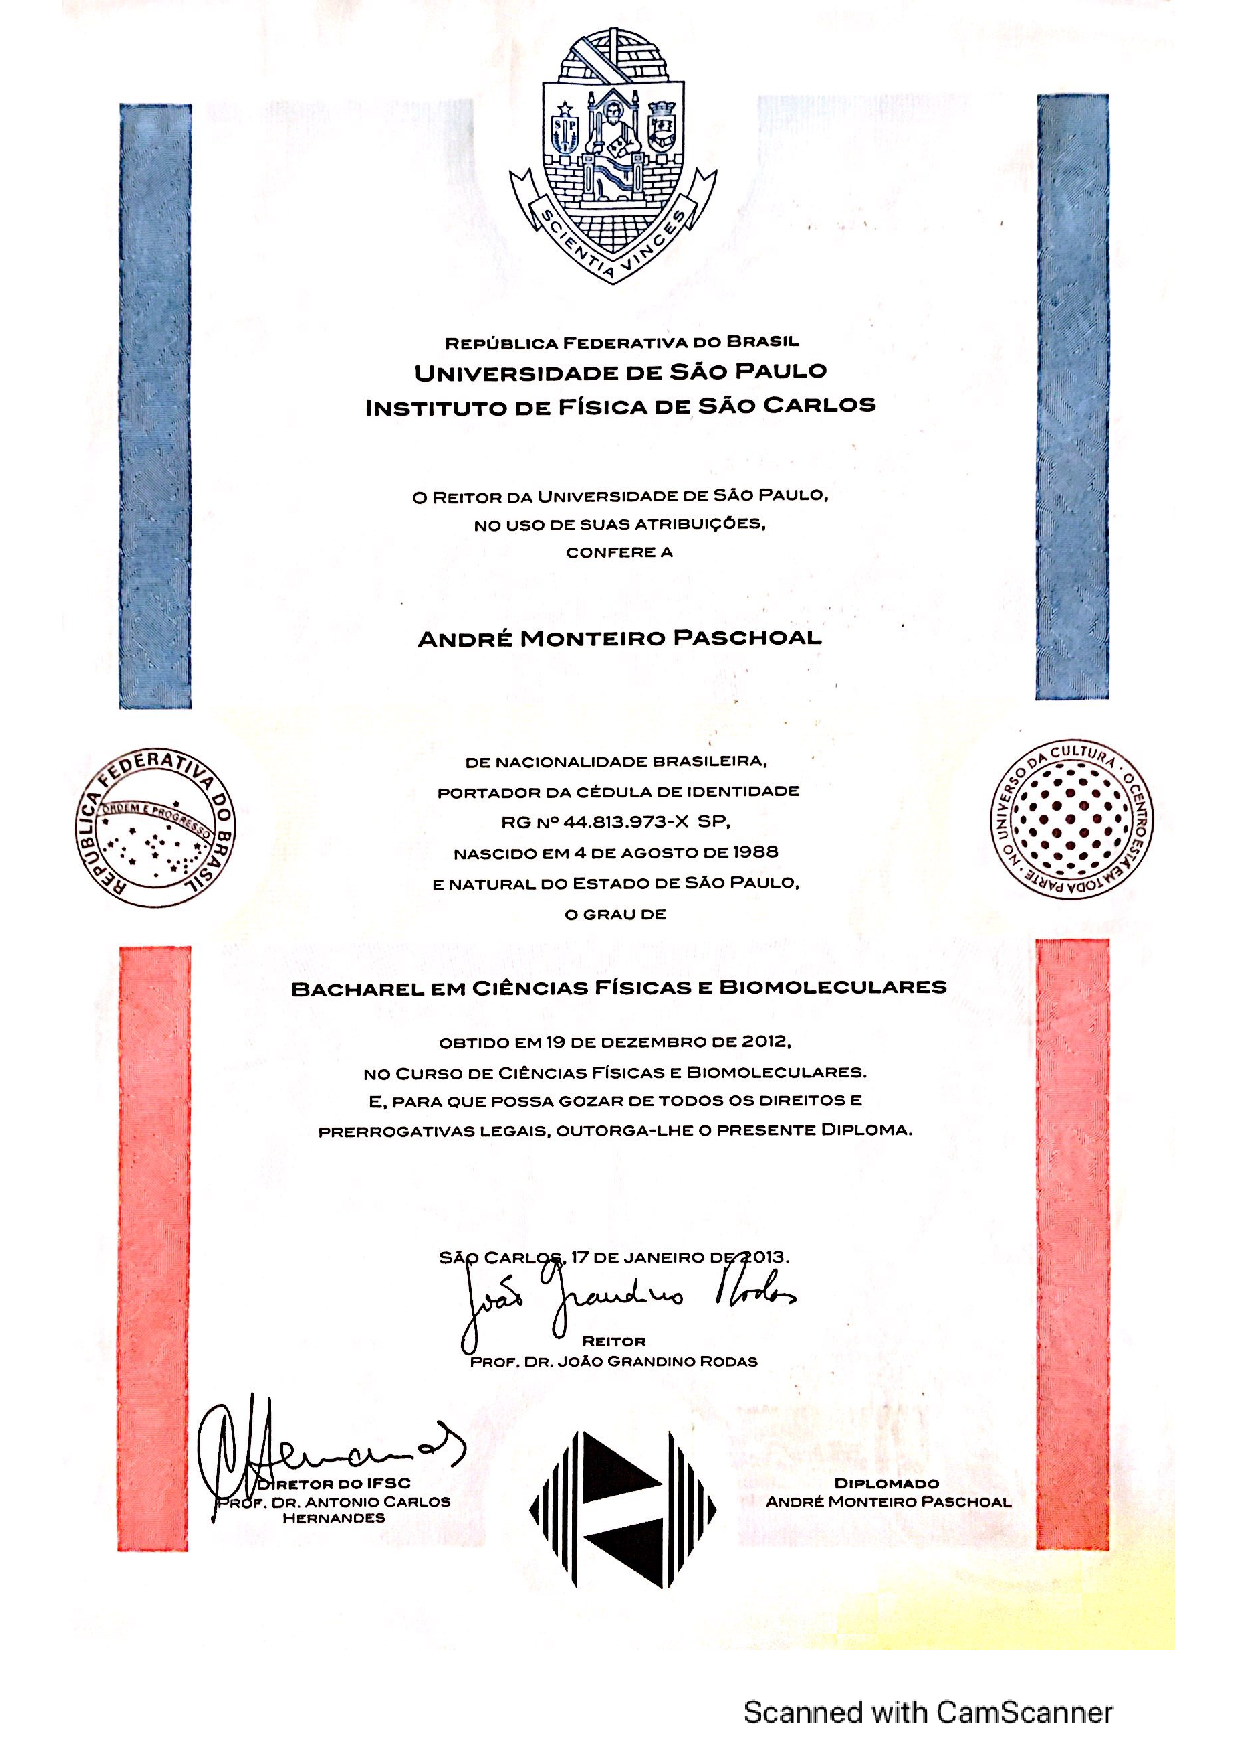
\includepdf[pages=-, scale=1,pagecommand=\thispagestyle{empty}]{\detokenize{Diplomas/DiplomaGraduaca}}

\newpage
\subsection{Atestado de estágio de iniciação científica no Laboratório de Química Medicinal e Computacional, localizado no 
Instituto de Física de São Carlos (IFSC - USP)}
\label{diplomas:IC}
Esta subseção apresenta o atestado de realização de iniciação científica no Laboratório de Química Medicinal e Computacional, localizado no 
Instituto de Física de São Carlos (IFSC - USP), desenvolvendo o projeto "Avaliação Biológica de Novos Agentes Anticâncer" sob orientação do Prof. 
Dr. Adriano D. Andricopulo no período de janeiro à dezembro de 2009.
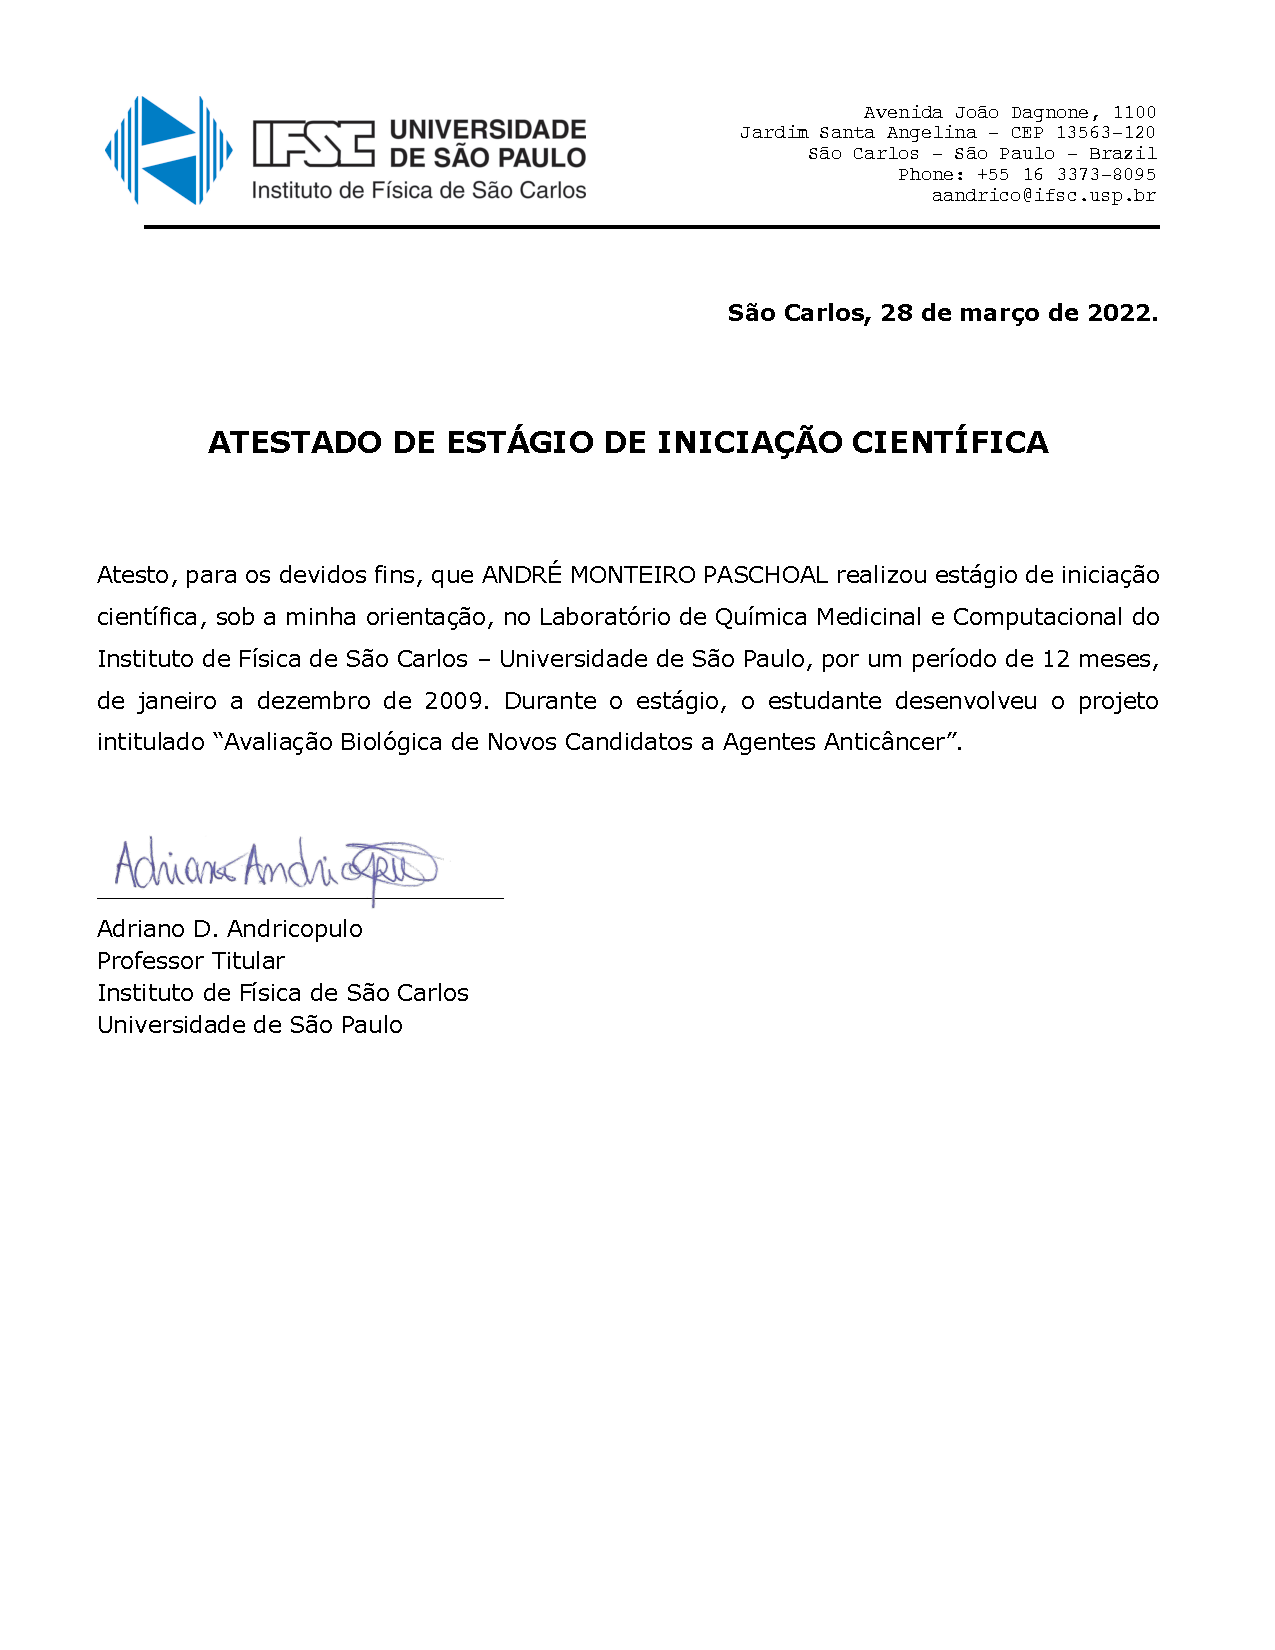
\includepdf[pages=-, scale=1,pagecommand=\thispagestyle{empty}]{\detokenize{Diplomas/IC_IFSC}}

\newpage
\subsection{Diploma de Mestre em Ciências, junto ao Instituto de Física de São Carlos (IFSC - USP)}
\label{diplomas:mestrado}
Esta subseção apresenta o diploma de Mestre em Ciências do candidato.
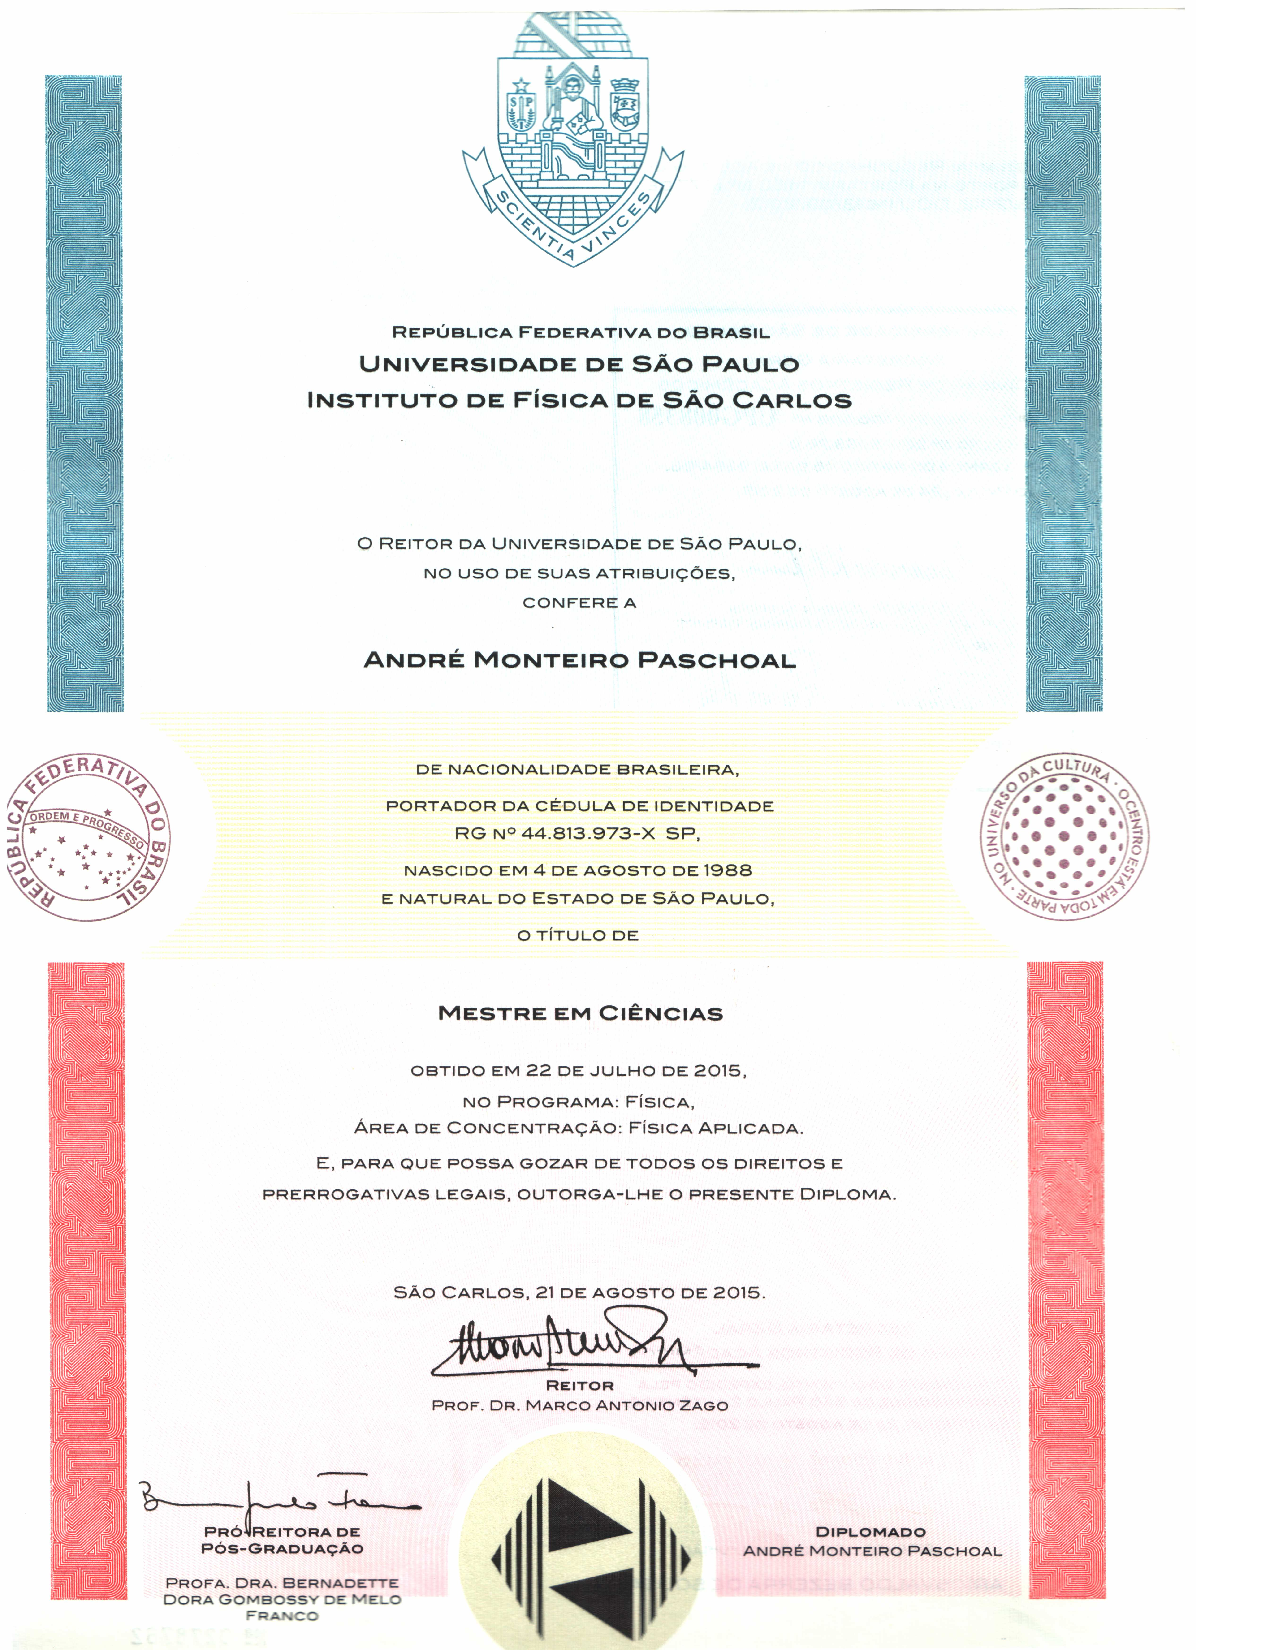
\includepdf[pages=-, scale=1,pagecommand=\thispagestyle{empty}]{\detokenize{Diplomas/diploma-mestrado}}

\newpage
\subsection{Diploma de Doutor em Ciências, junto ao Departamento de Física da Faculdade de Filosofia, Ciências e Letras de Ribeirão Preto (FFCLRP) da Universidade de São Paulo (USP)}
\label{diplomas:doutorado}
Esta subseção apresenta o diploma de Doutor em Ciências do candidato.
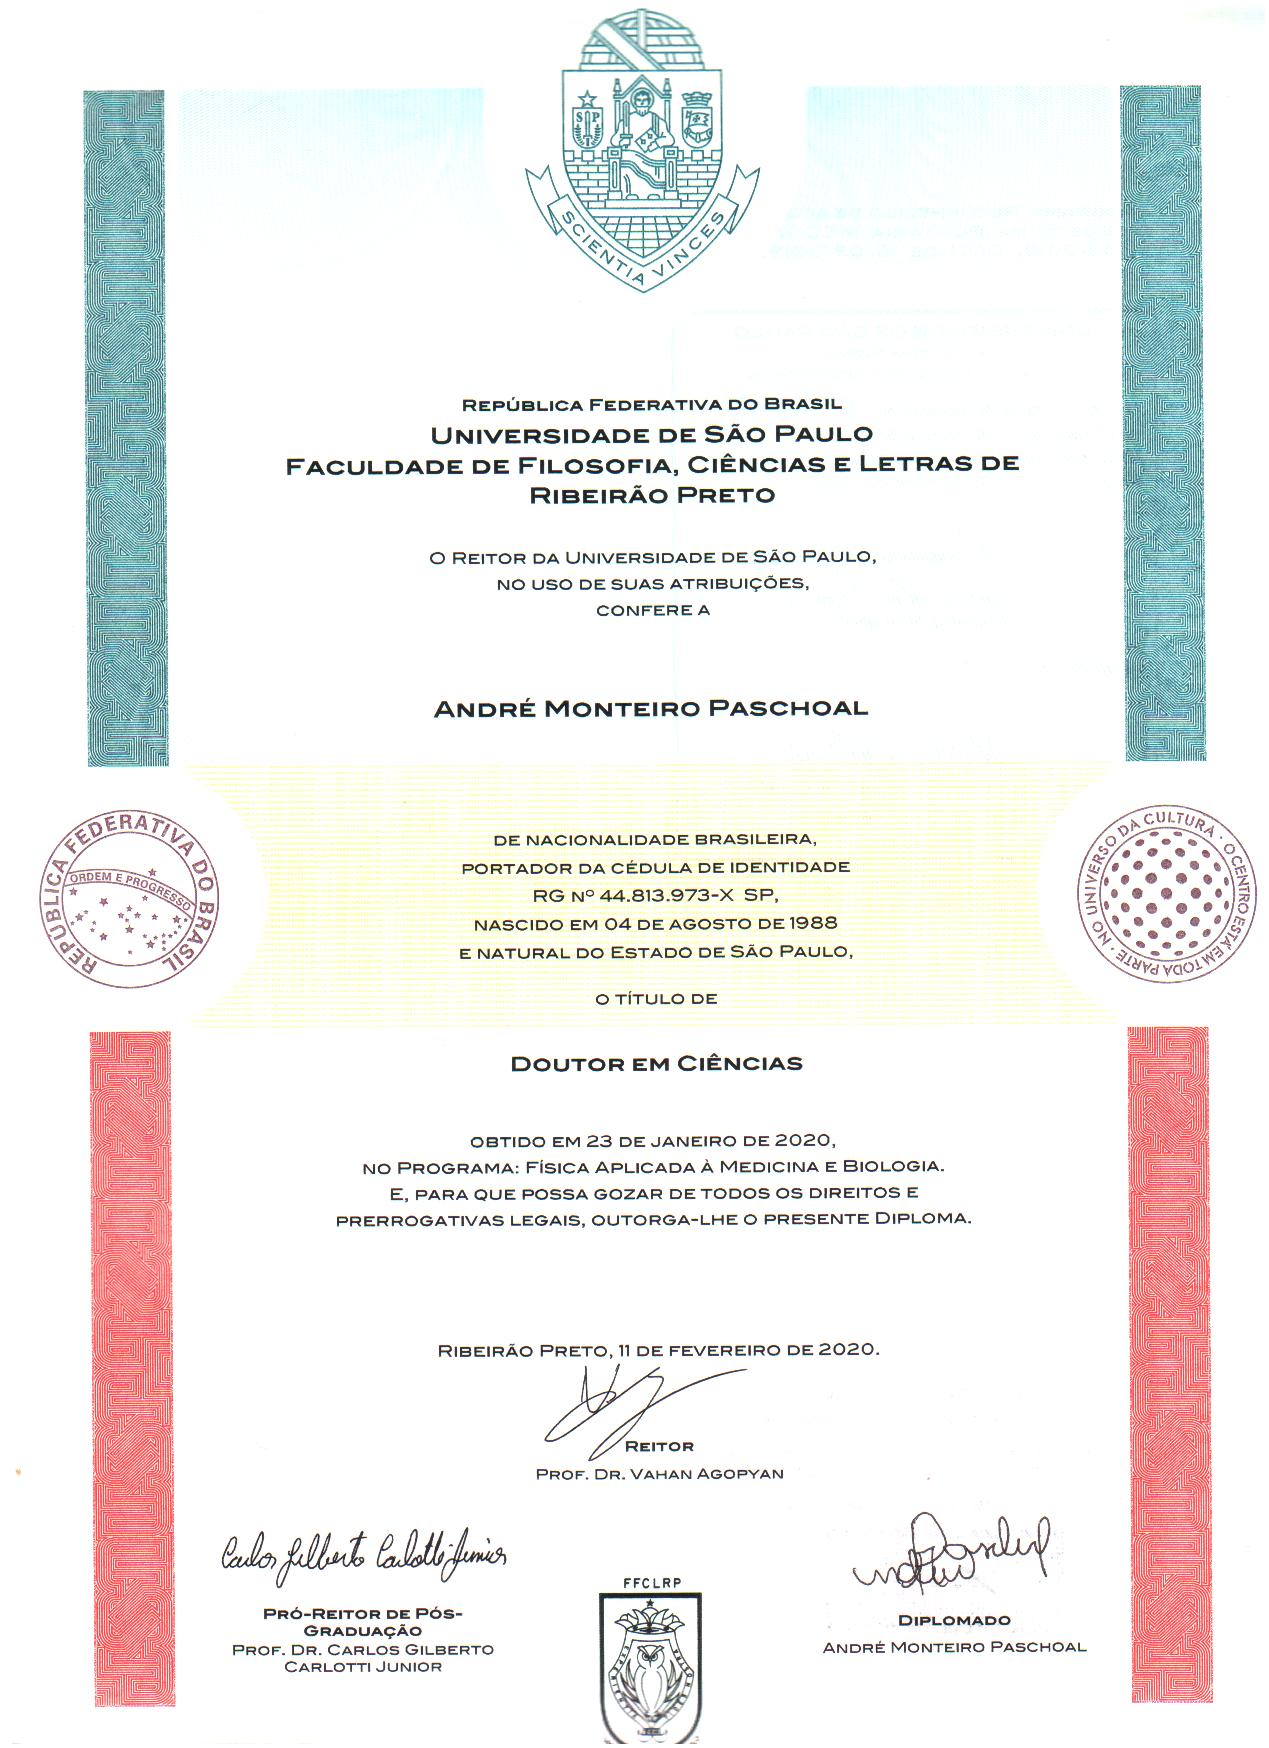
\includepdf[pages=-, scale=1,pagecommand=\thispagestyle{empty}]{\detokenize{Diplomas/PhDcertificate}}

\newpage
\subsection{Certificado de Pós Doutorado, junto à Faculdade de Medicina de Ribeirão Preto (FMRP) da Universidade de São Paulo (USP)}
\label{diplomas:posdoc1}
Esta subseção apresenta o certificado de conclusão do pós doutorado junto à FMRP do candidato.
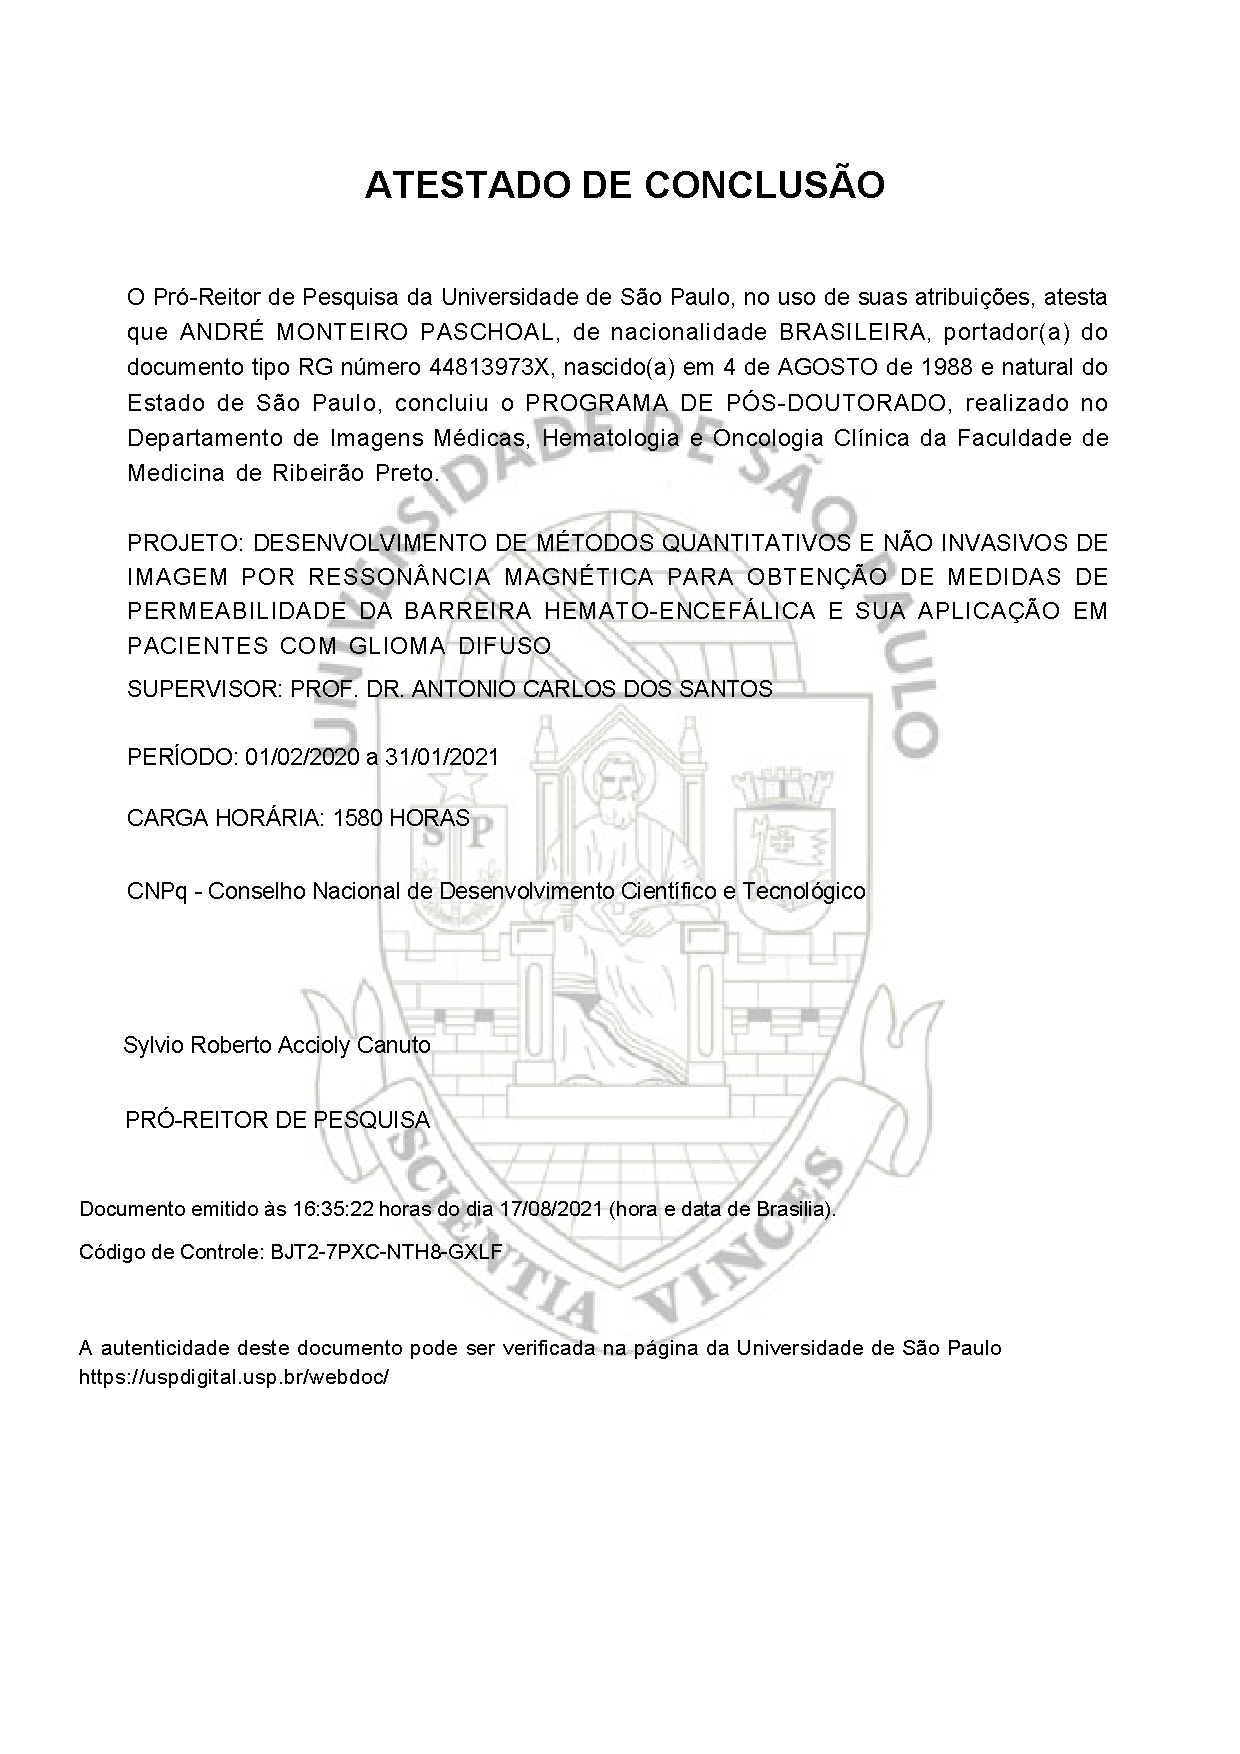
\includepdf[pages=-, scale=1,pagecommand=\thispagestyle{empty}]{\detokenize{Diplomas/posdocFMRP}}

\newpage
\subsection{Declaração de pesquisador, junto à Faculdade de Medicina da Universidade de São Paulo (FMUSP)}
\label{diplomas:posdoc2}
Esta subseção apresenta a declaração das atividades do candidato como pesquisador no Instituto de Radiologia, da Faculdade de Medicina da Universidade de São 
Paulo.
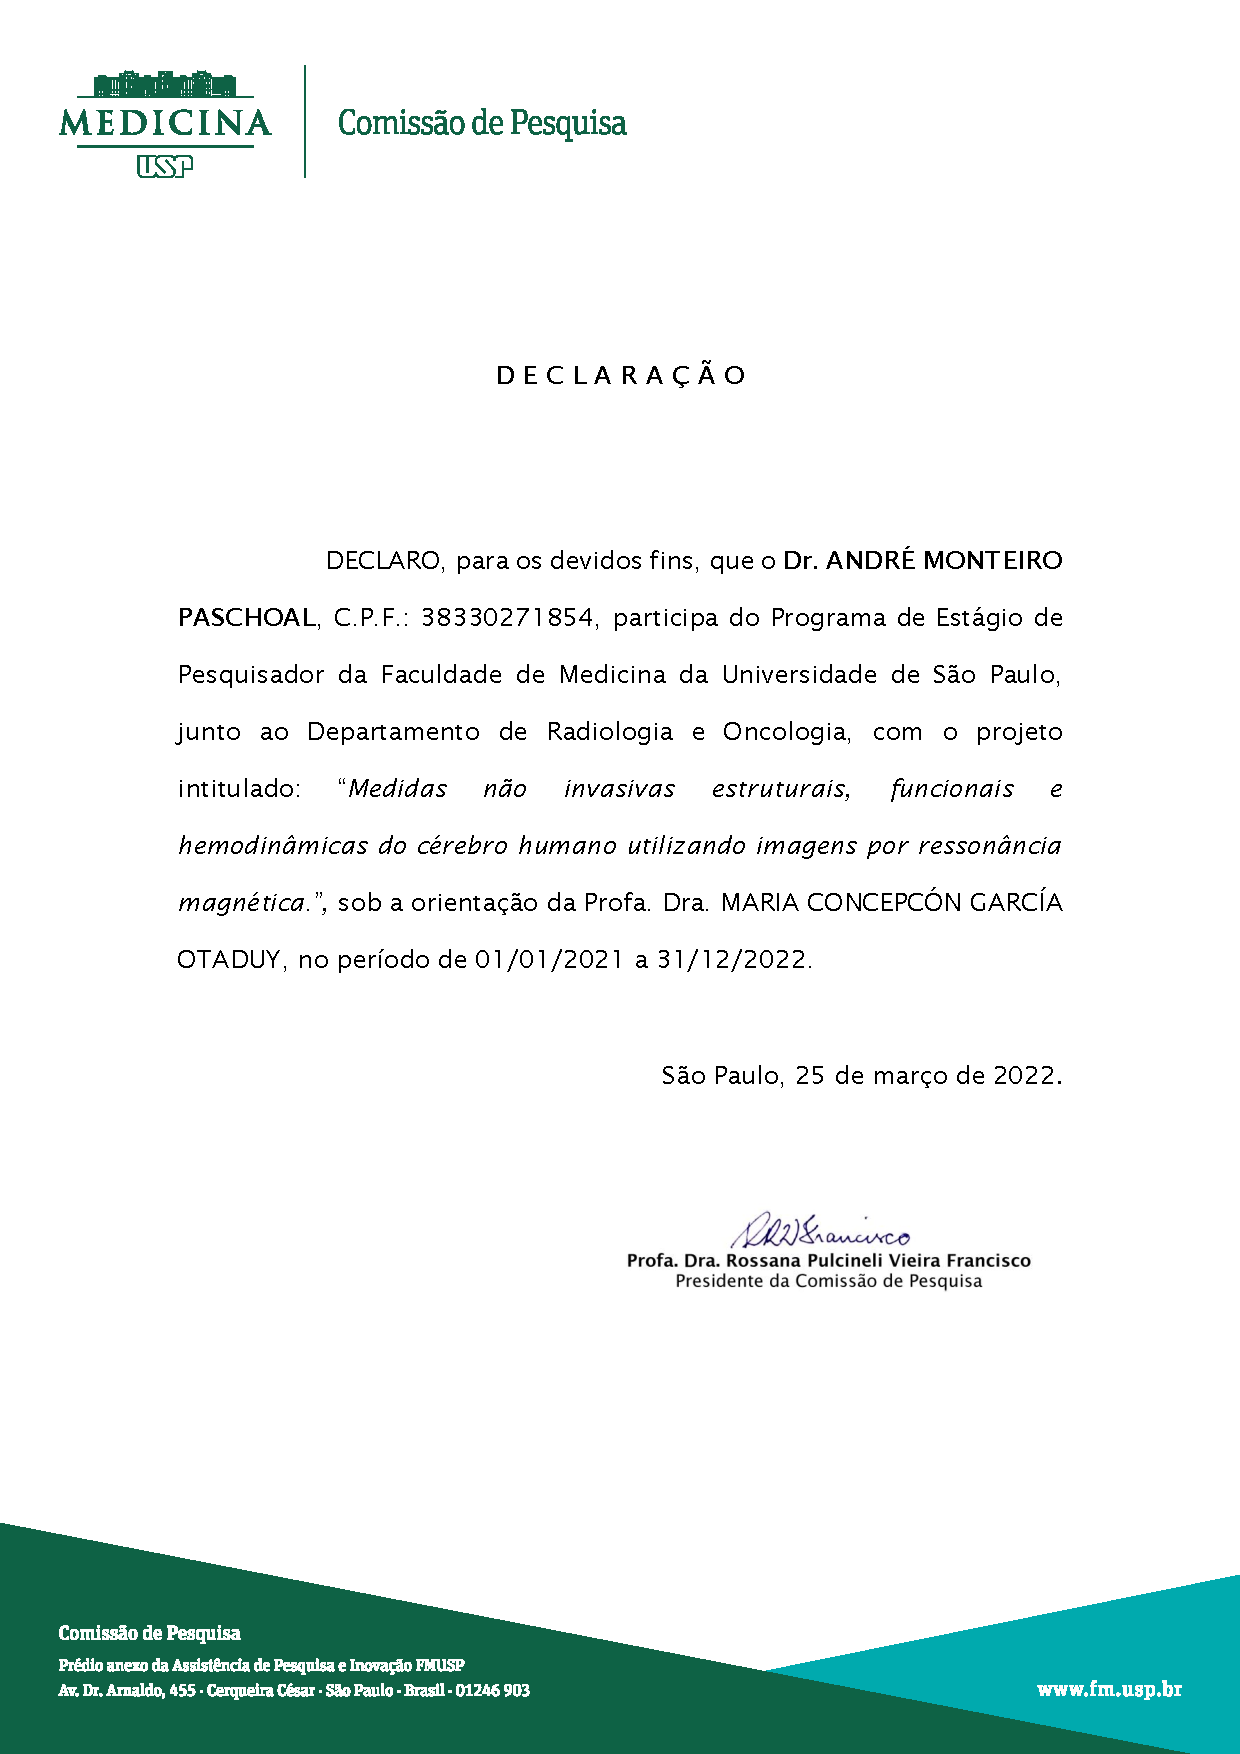
\includepdf[pages=-, scale=1,pagecommand=\thispagestyle{empty}]{\detokenize{Diplomas/declaracaoEstagioInRad}}

\newpage
\subsection{Participação como pesquisador associado no projeto FAPESP número 2019/06148-6}
\label{certificados:fapesp_regular2019}
Esta subseção apresenta o comprovante de participação como pesquisador associado no projeto FAPESP número 2019/06148-6.
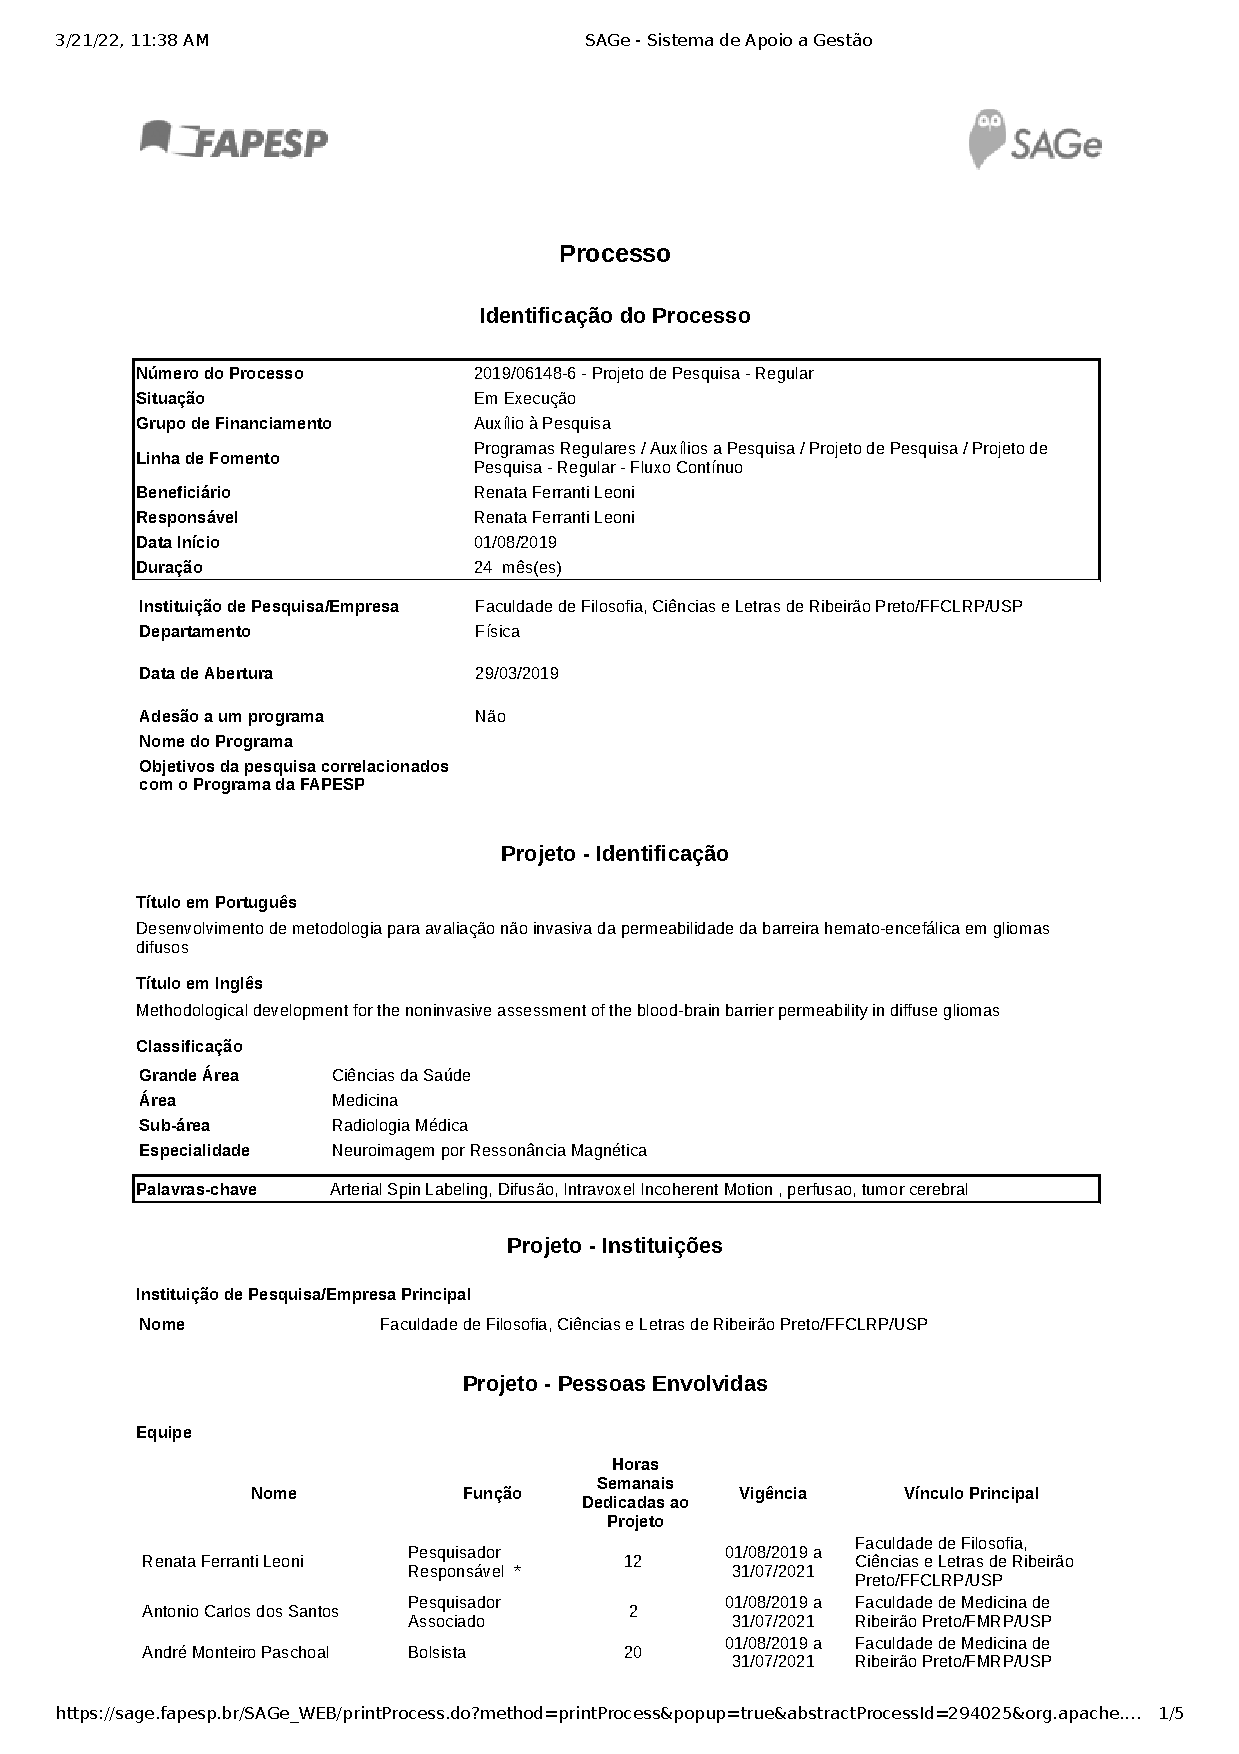
\includepdf[pages=-, scale=1,pagecommand=\thispagestyle{empty}]{\detokenize{Diplomas/fapesp_renata2019}}

\newpage
\subsection{Declaração de realização de estágio remunerado}
\label{declaracao:SAPRA}
Esta subseção apresenta a declaração de realização de estágio remunerado na empresa SAPRA-Landauer Serviço de Assessoria e Proteção Radiológica Ltda no período 
de 08 de fevereiro à 07 de dezembro de 2012.
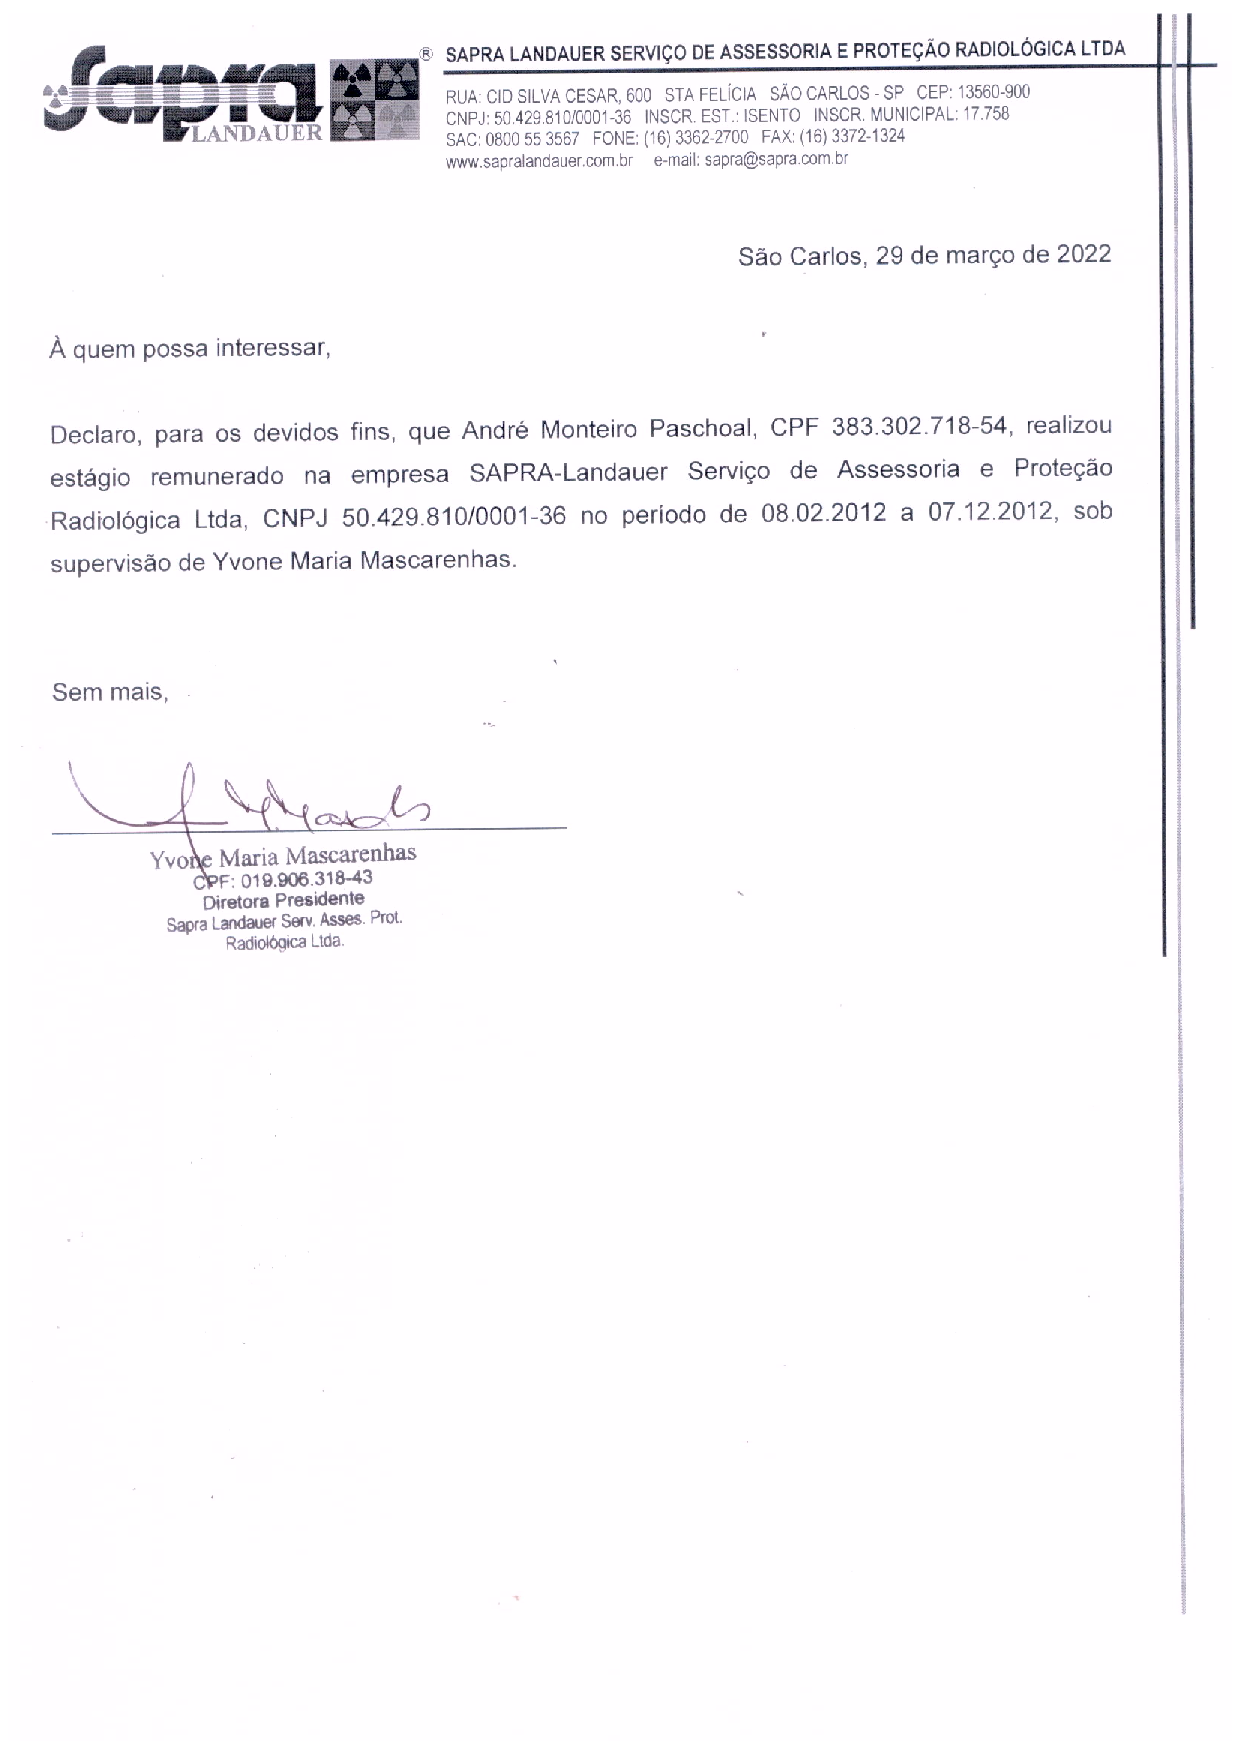
\includepdf[pages=-, scale=1,pagecommand=\thispagestyle{empty}]{\detokenize{Diplomas/estagioSAPRA}}

\newpage
\subsection{Certificado de conclusão do MRI Graduate Program pela Universidade de Oxford}
\label{diplomas:oxford}
Esta subseção apresenta o comprovante de conclusão do curso MRI \textit{Graduate Program}, oferecido pelo programa WIN da Universidade de Oxford, 
com duração de um ano.
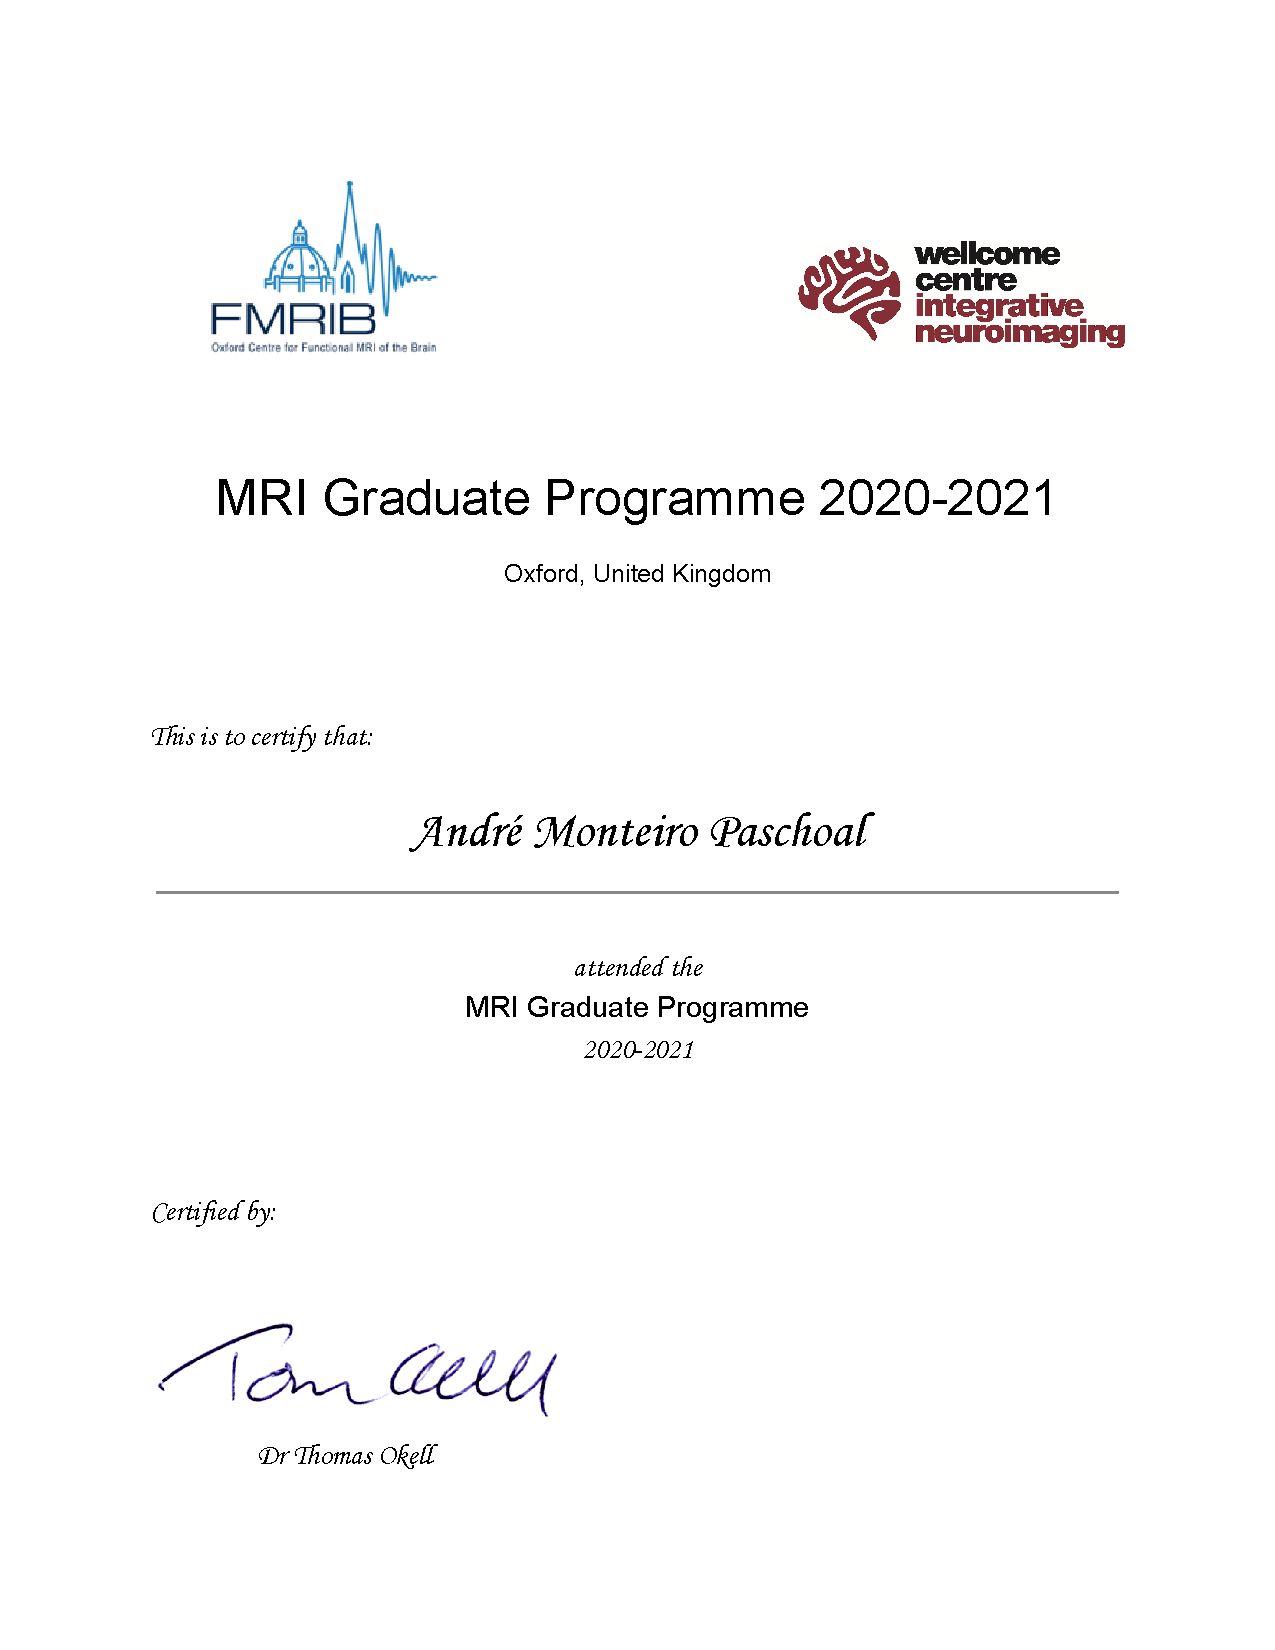
\includepdf[pages=-, scale=1,pagecommand=\thispagestyle{empty}]{\detokenize{Diplomas/MRIoxford}}

\newpage
\subsection{Prêmios de mérito científico}
\label{awards:OHBM}
Esta subseção apresenta o certificado de obtenção do Prêmio \textbf{OHBM Travel Award}, concedido no Encontro Anual da \textit{Organization for Human Brain Mapping} no ano de 2019, realizado em Roma - Itália.
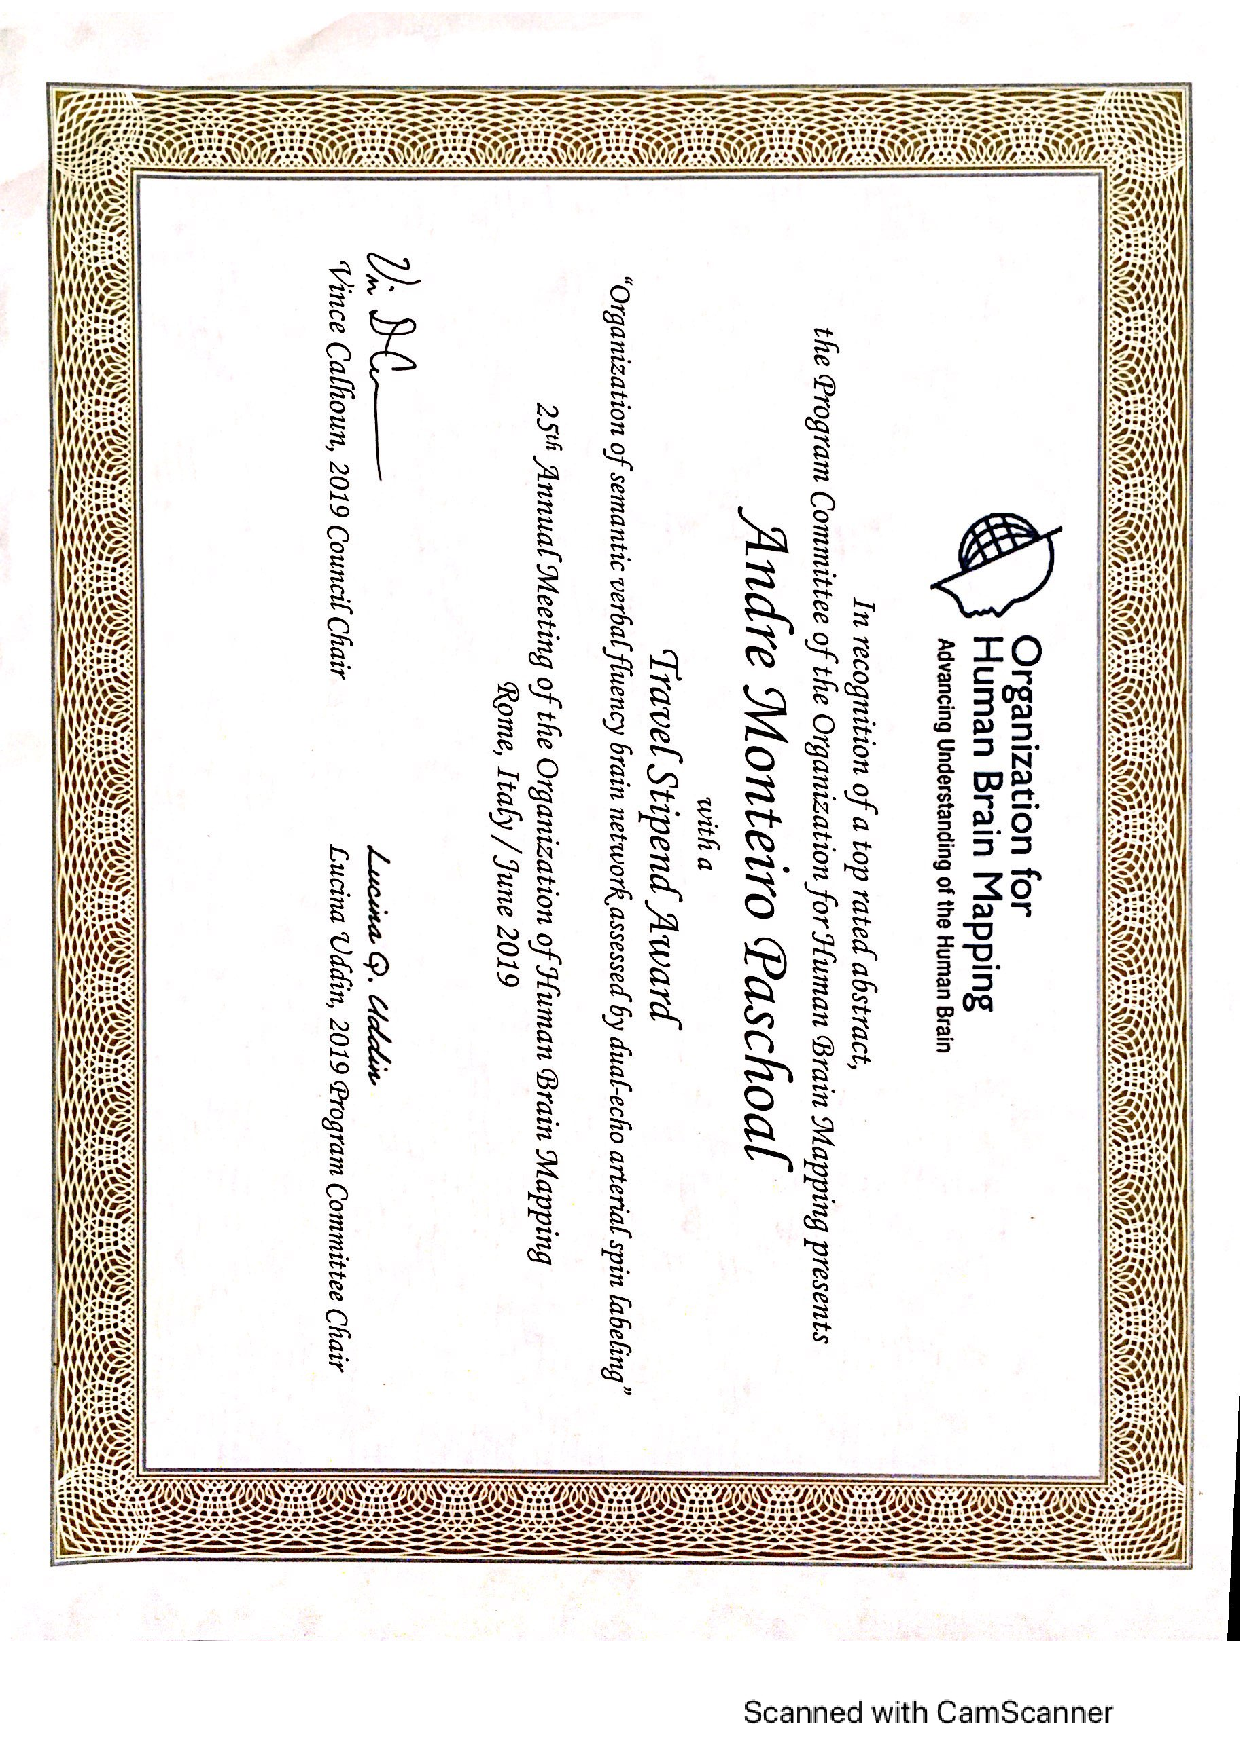
\includepdf[pages=-, scale=1,pagecommand=\thispagestyle{empty}]{\detokenize{Diplomas/OHBMtravelAward}}

\newpage
\subsection{Prêmios de mérito científico - Prêmio CAPES de Teses}
\label{awards:CAPES}
Esta subseção apresenta o certificado de obtenção da Menção Honrosa no \textbf{Prêmio CAPES de Teses 2021}, concedido pela CAPES no ano de 2021.
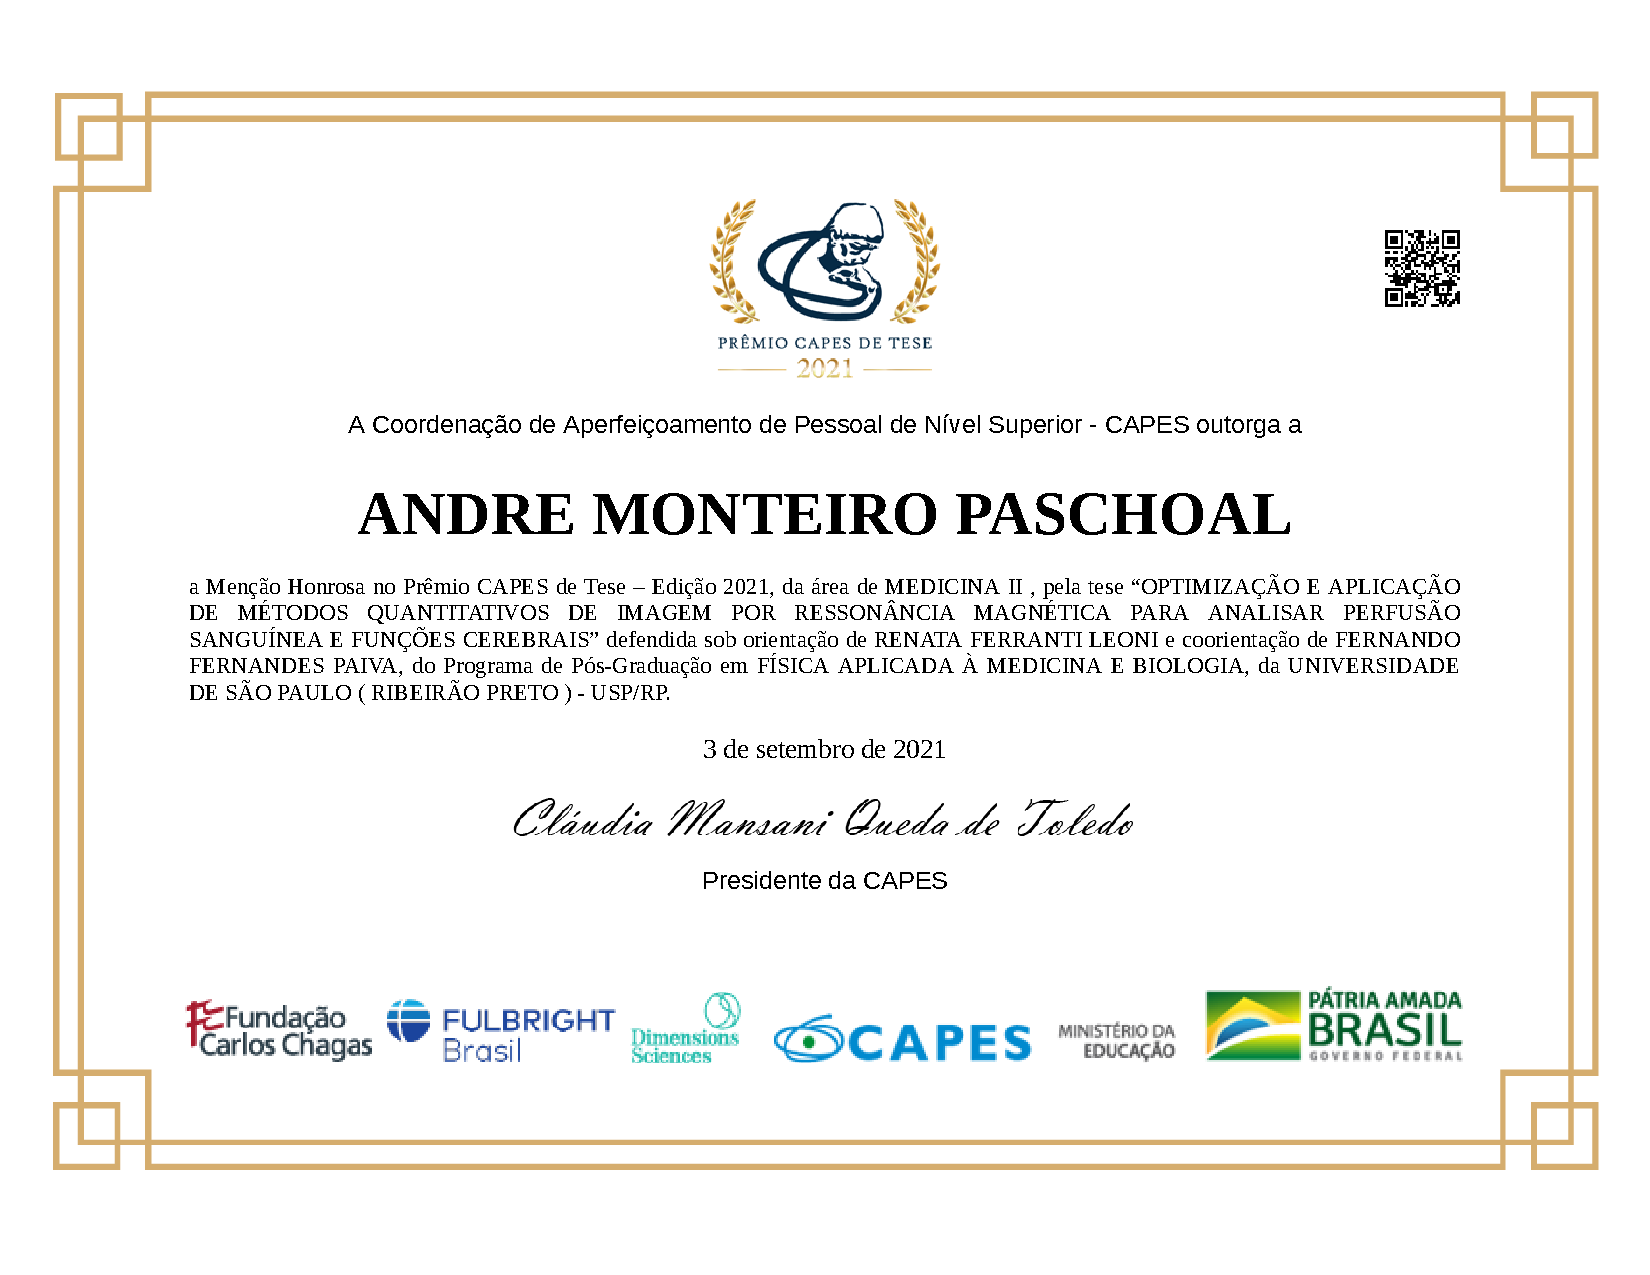
\includepdf[pages=-, scale=1,pagecommand=\thispagestyle{empty}]{\detokenize{Diplomas/premioCAPES}}

%%%%%%%%%%%%%%%%%%%%%%%%%%%%%%%%%%%%%%%%%%%%%%%%%%%%%%%%%%%%%%%%%%%%%%%%%%%%%%%
% Subgrupo 2.1 - Produtividade de Pesquisa
%%%%%%%%%%%%%%%%%%%%%%%%%%%%%%%%%%%%%%%%%%%%%%%%%%%%%%%%%%%%%%%%%%%%%%%%%%%%%%%

\newpage
\subsection{Participa\c{c}\~{a}o em Eventos Cient\'{\i}ficos (com apresenta\c{c}\~{a}o de trabalho ou oferecimento de cursos, palestras ou debates}
\label{certificados:SIFSC2013}
Esta subseção apresenta o comprovante da participação na III Semana Integrada do Instituto de Física de São Carlos com seus respectivos propósitos.
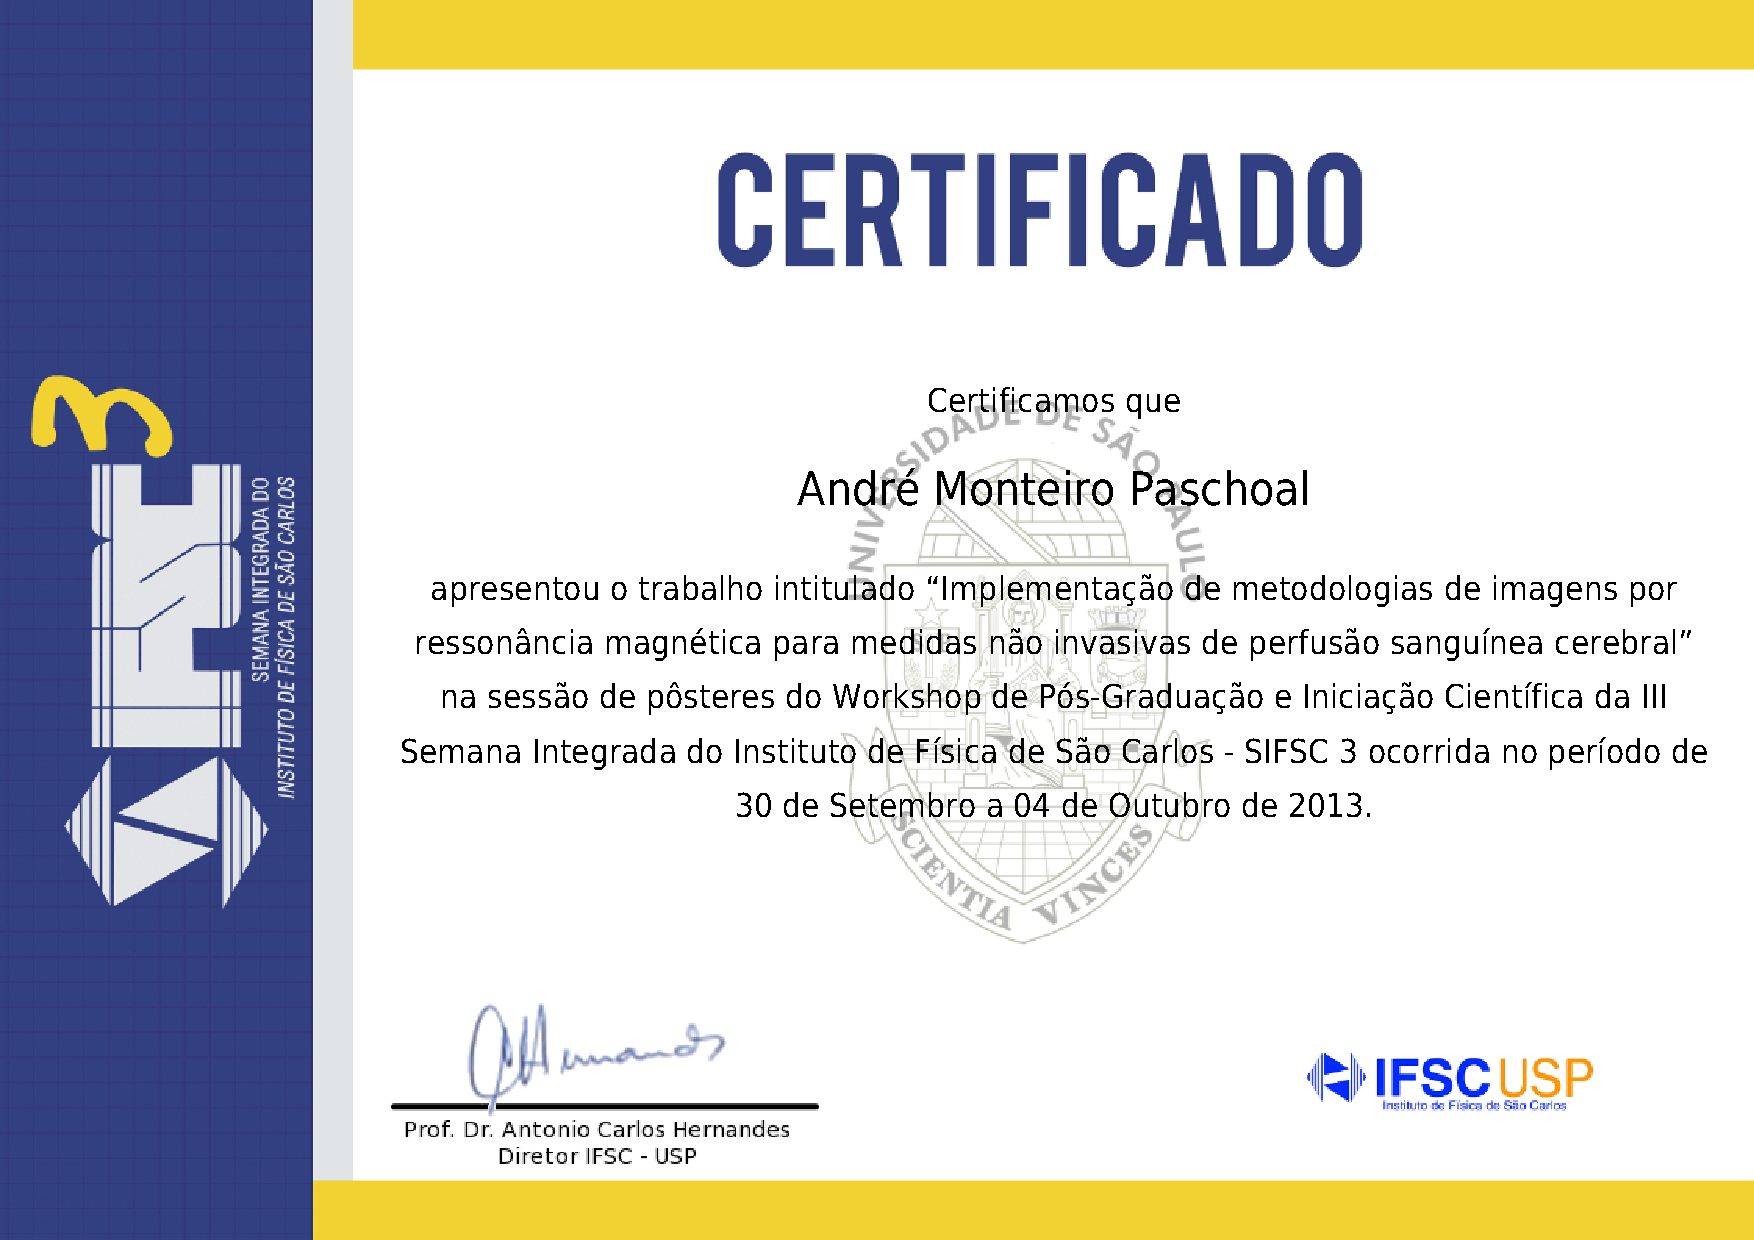
\includepdf[pages=-, scale=1,pagecommand=\thispagestyle{empty}]{\detokenize{Diplomas/CertificadoSIFSC2013}}

\newpage
\subsection{Participa\c{c}\~{a}o em Eventos Cient\'{\i}ficos (com apresenta\c{c}\~{a}o de trabalho ou oferecimento de cursos, palestras ou debates}
\label{certificados:SIFSC2014}
Esta subseção apresenta o comprovante da participação na IV Semana Integrada do Instituto de Física de São Carlos com seus respectivos propósitos.
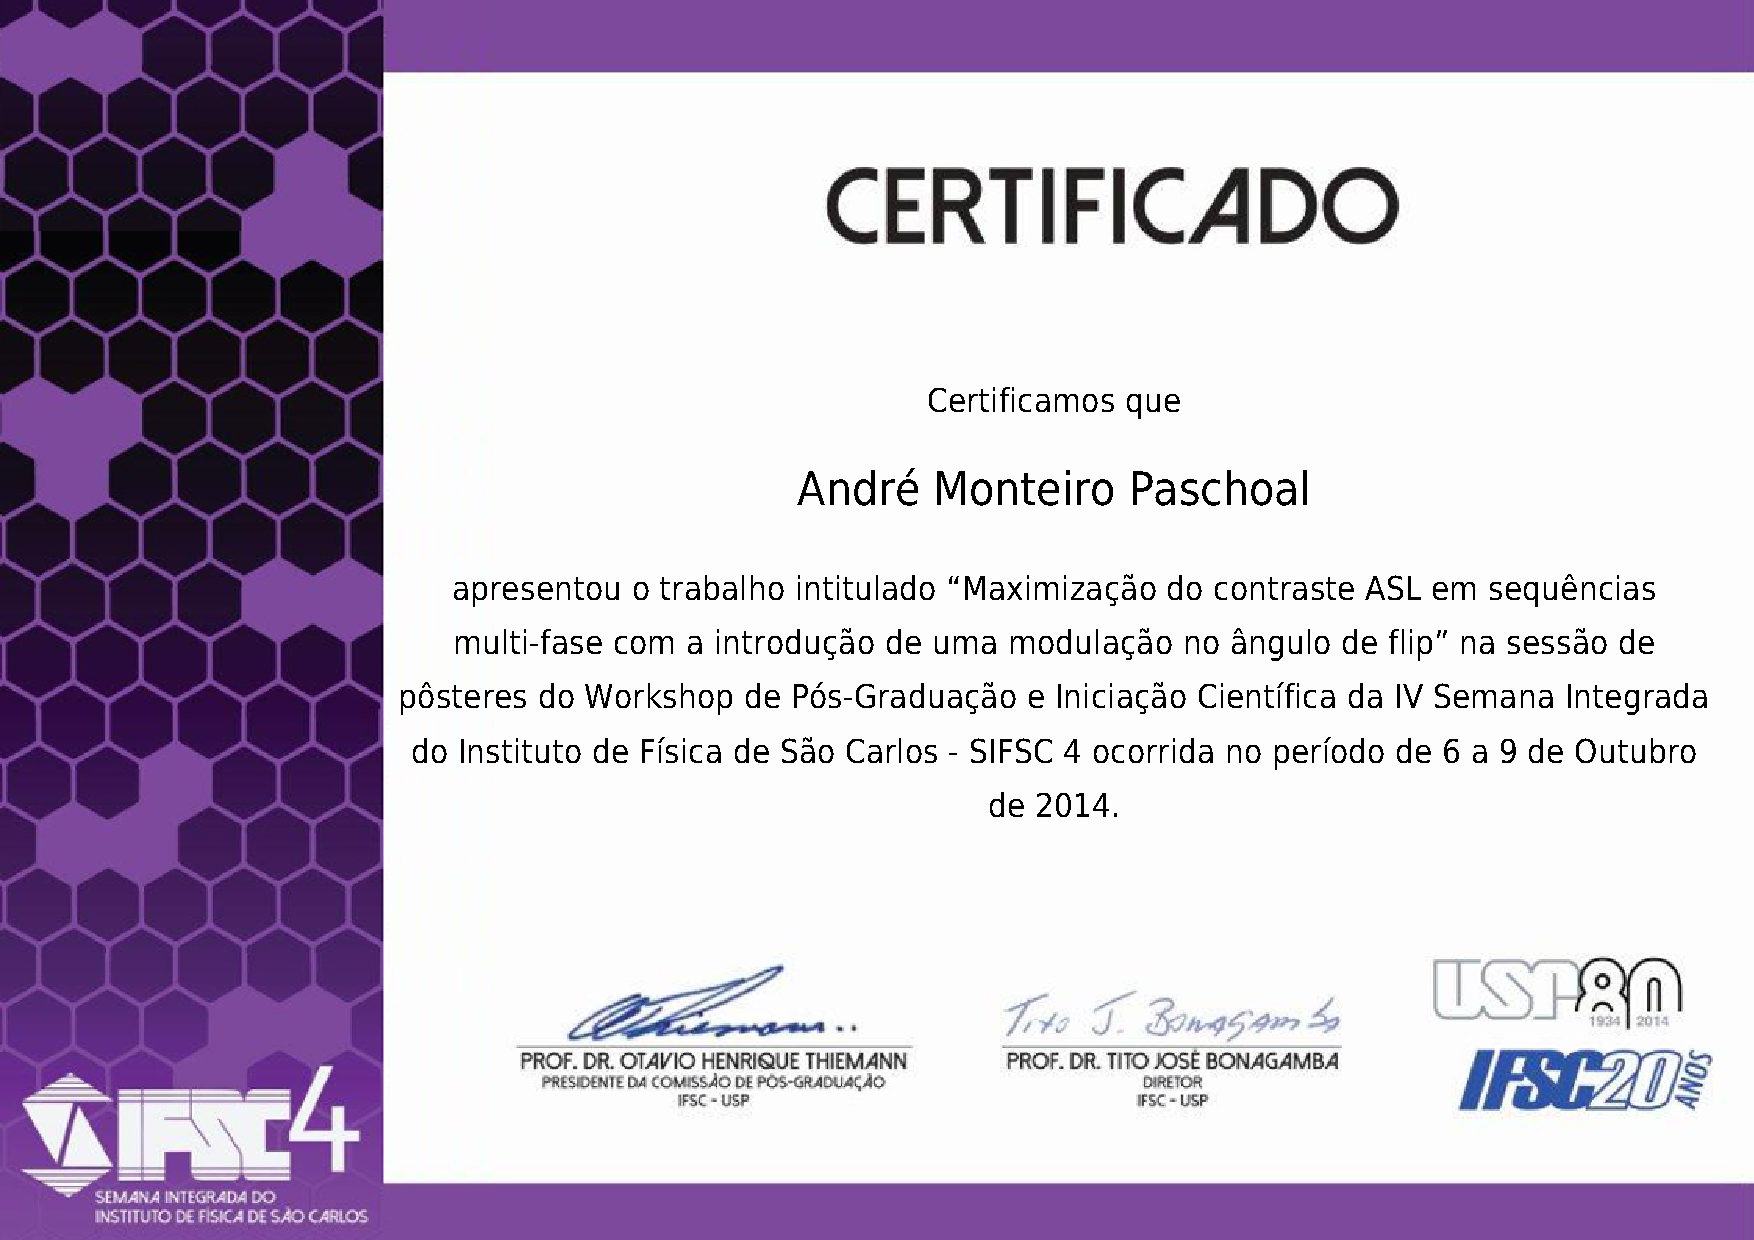
\includepdf[pages=-, scale=1,pagecommand=\thispagestyle{empty}]{\detokenize{Diplomas/CertificadoSIFSC2014}}

\newpage
\subsection{Participa\c{c}\~{a}o em Eventos Cient\'{\i}ficos (com apresenta\c{c}\~{a}o de trabalho ou oferecimento de cursos, palestras ou debates}
\label{certificados:Transatlantic}
Esta subseção apresenta o comprovante da participação no I Transatlantic Workshop on Methods for Multimodal Neurosciences Studies com seus respectivos propósitos.
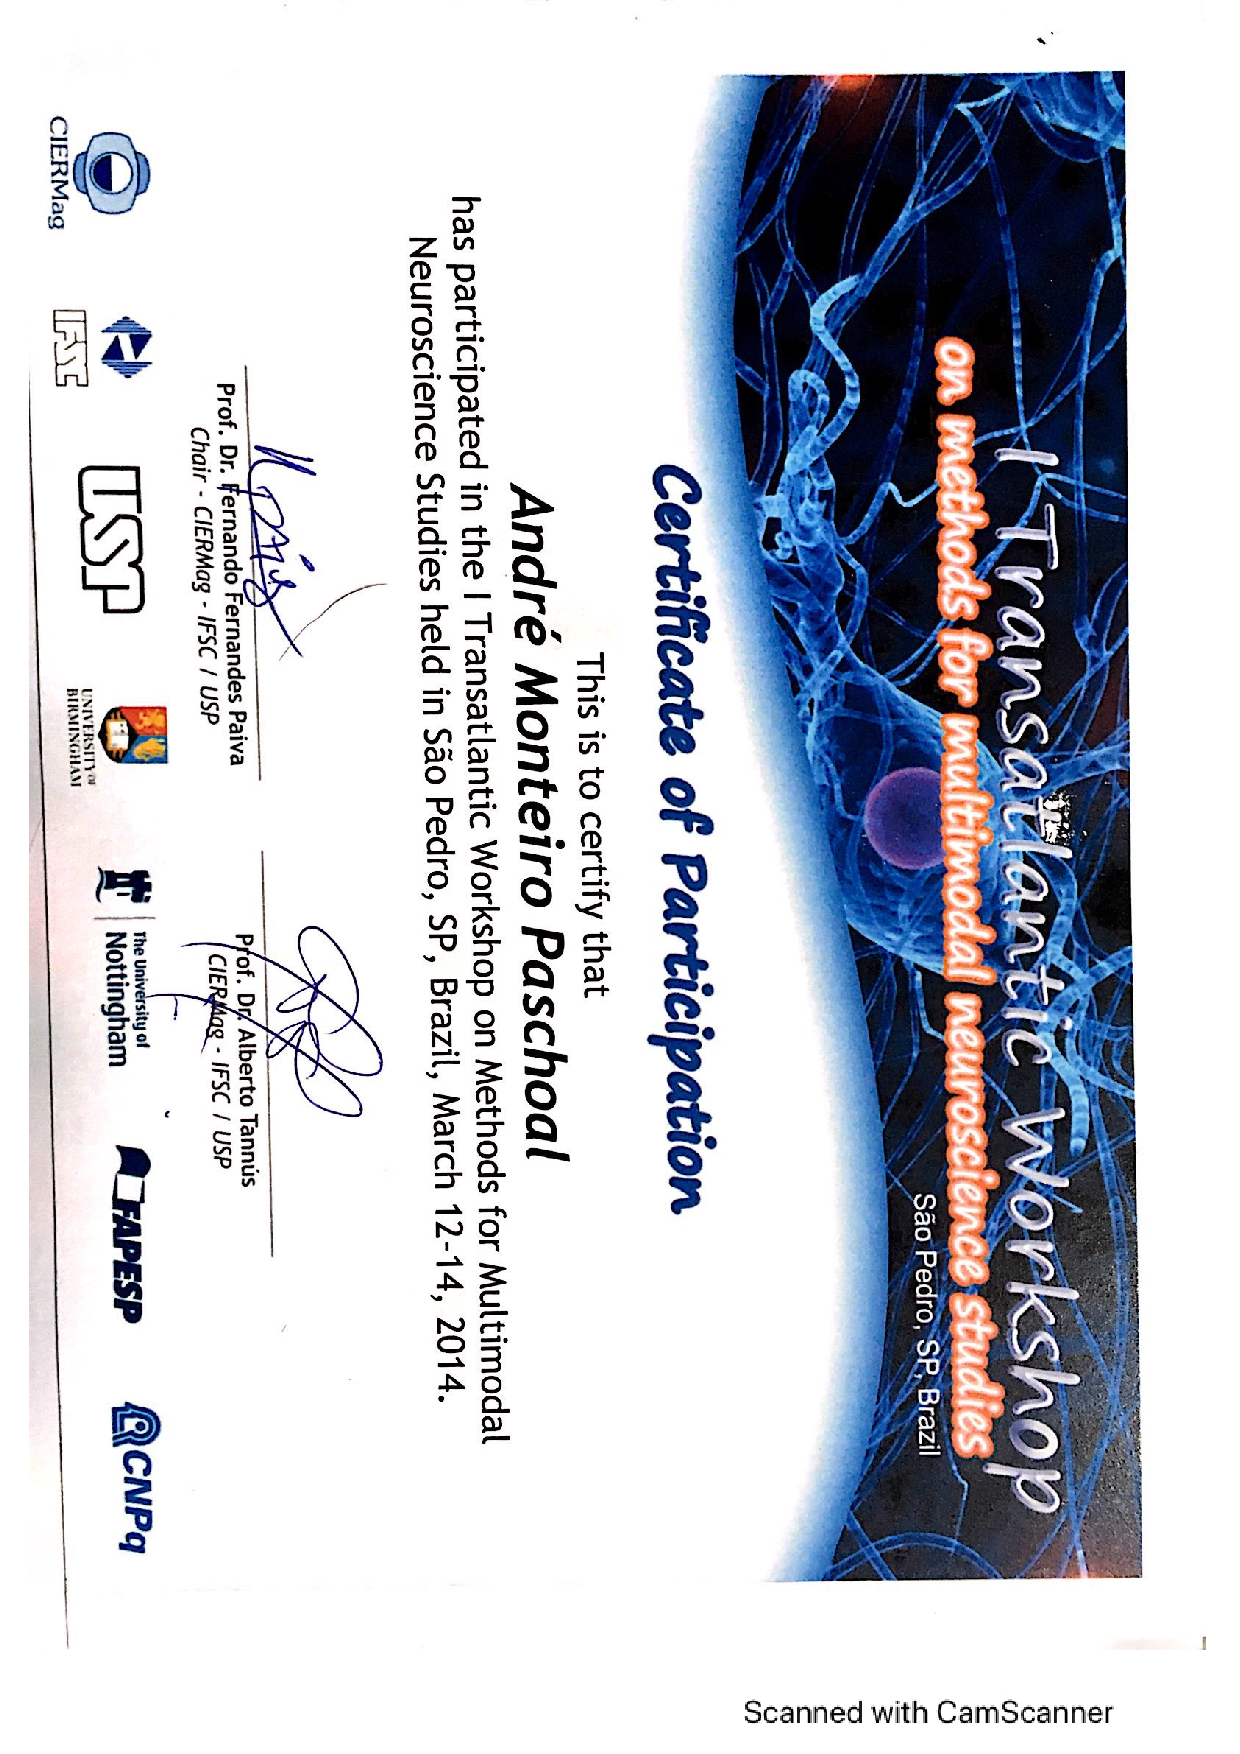
\includepdf[pages=-, scale=1,pagecommand=\thispagestyle{empty}]{\detokenize{Diplomas/TransatlanticWorkshopParticipation}}
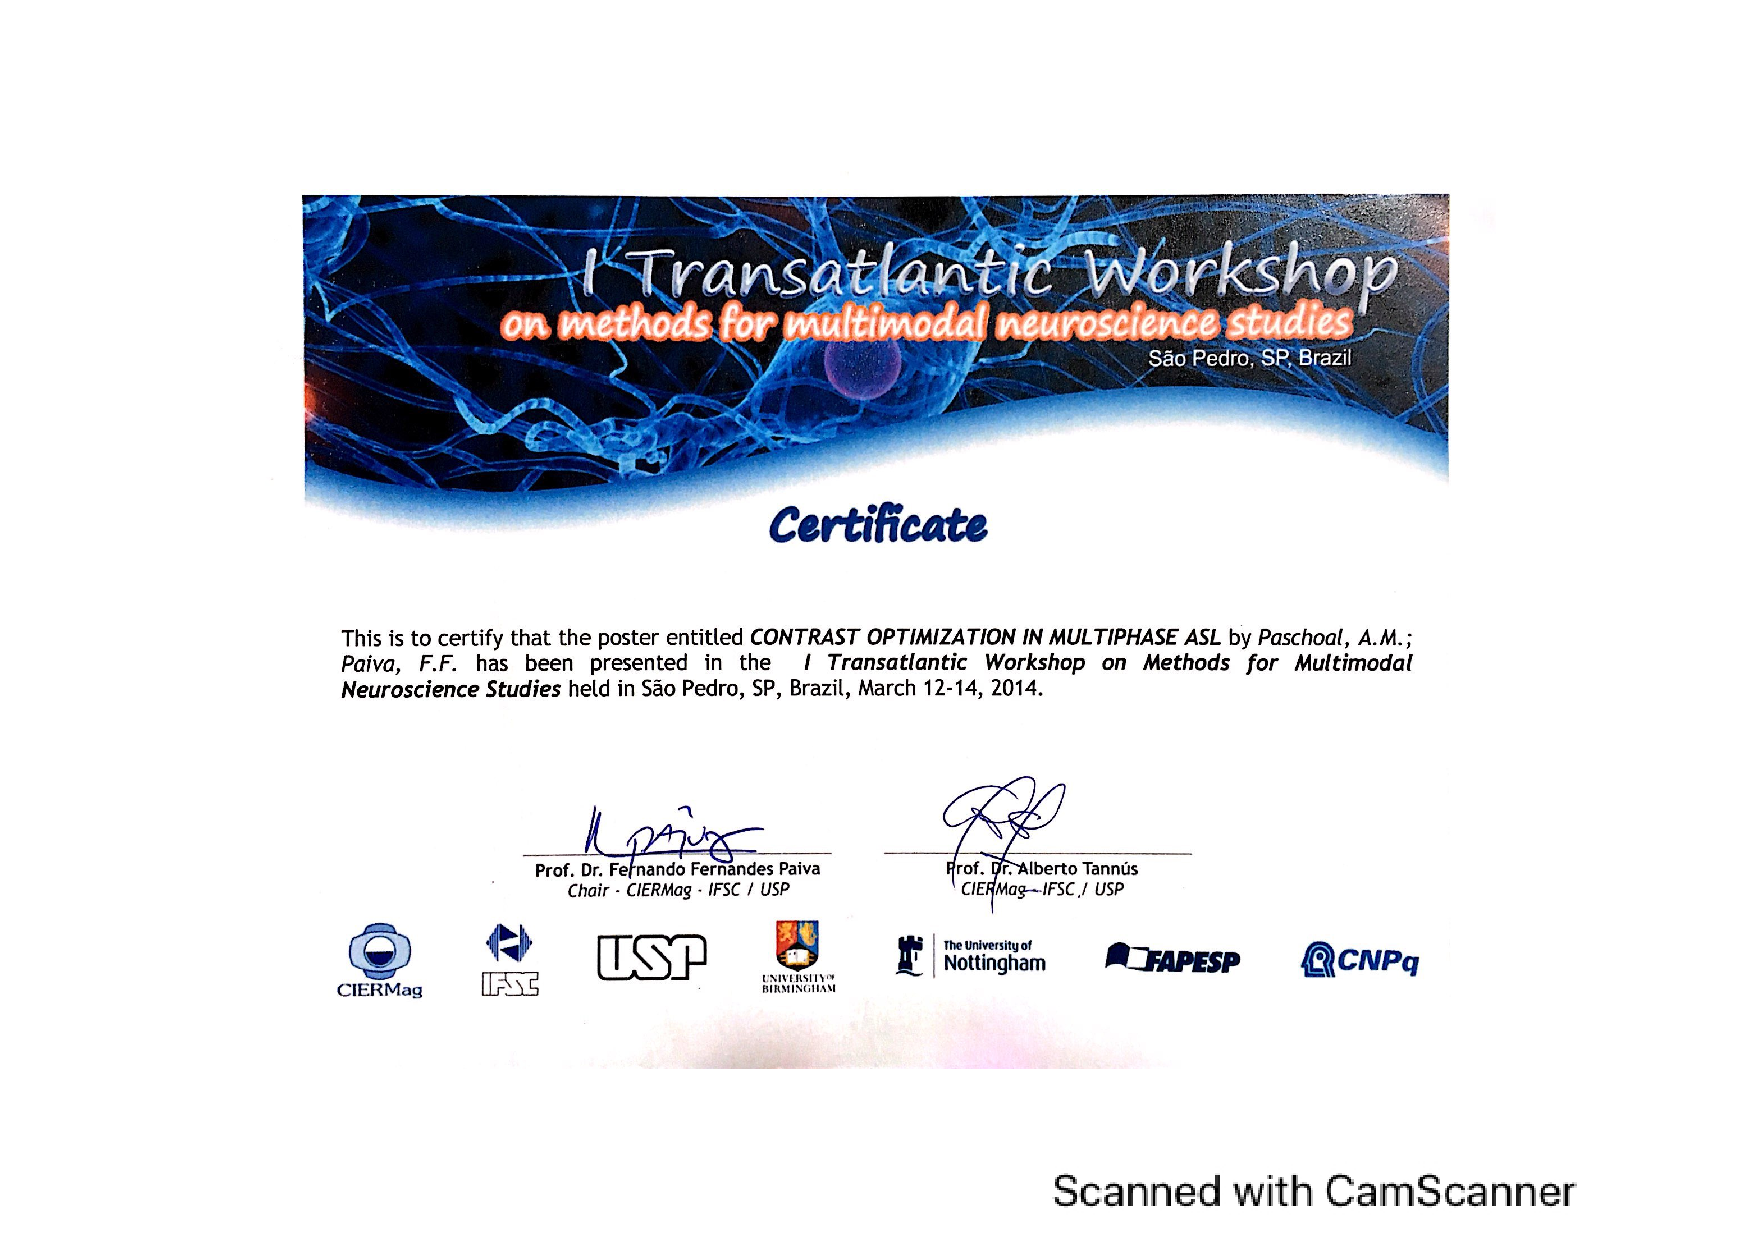
\includepdf[pages=-, scale=1,pagecommand=\thispagestyle{empty}]{\detokenize{Diplomas/TransatlanticWorkshopPresentation}}

\newpage
\subsection{Participa\c{c}\~{a}o em Eventos Cient\'{\i}ficos (com apresenta\c{c}\~{a}o de trabalho ou oferecimento de cursos, palestras ou debates}
\label{certificados:SIFSC2015}
Esta subseção apresenta o comprovante da participação na V Semana Integrada do Instituto de Física de São Carlos com seus respectivos propósitos.
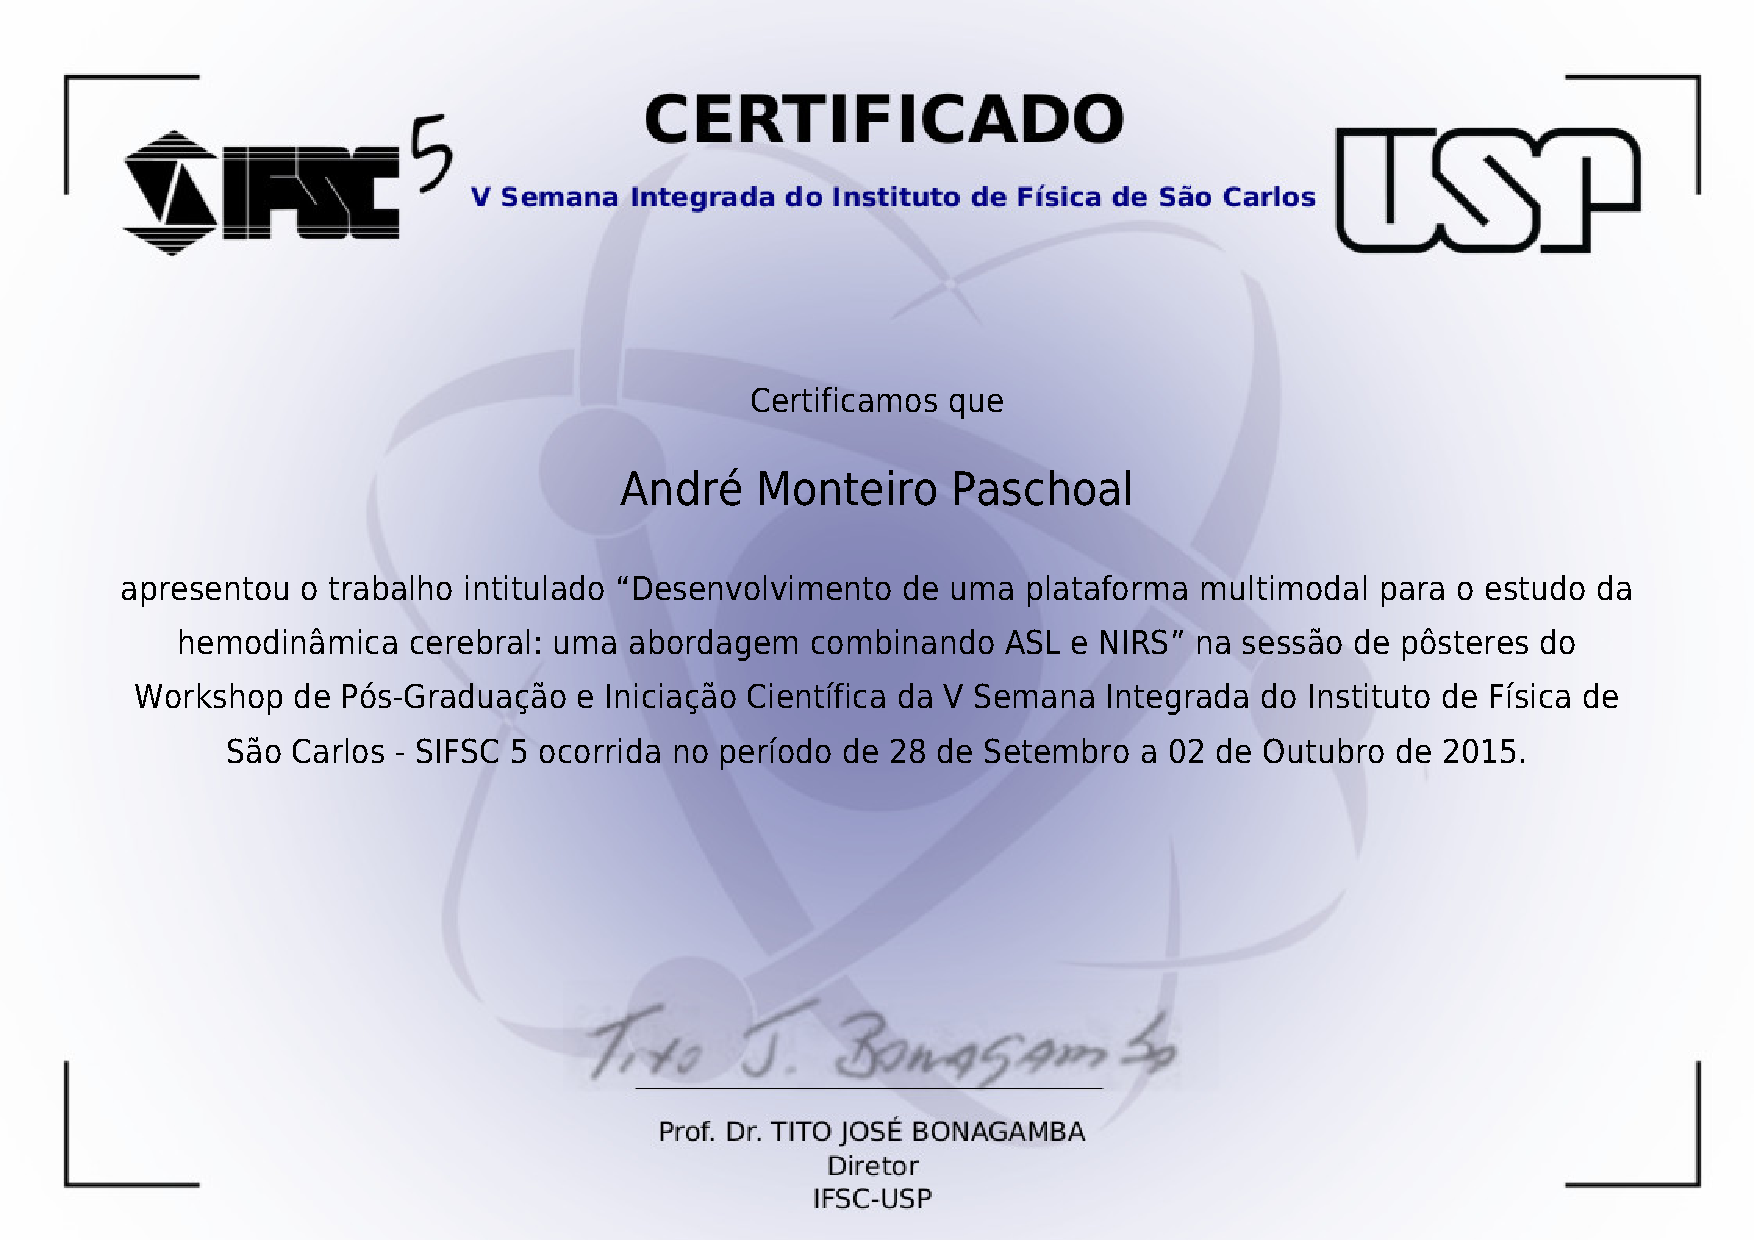
\includepdf[pages=-, scale=1,pagecommand=\thispagestyle{empty}]{\detokenize{Diplomas/CertificadoSIFSC2015}}

\newpage
\subsection{Participa\c{c}\~{a}o em Eventos Cient\'{\i}ficos (com apresenta\c{c}\~{a}o de trabalho ou oferecimento de cursos, palestras ou debates}
\label{certificados:SFM2016}
Esta subseção apresenta o comprovante da participação na XV Semana da Física Médica com seus respectivos propósitos.
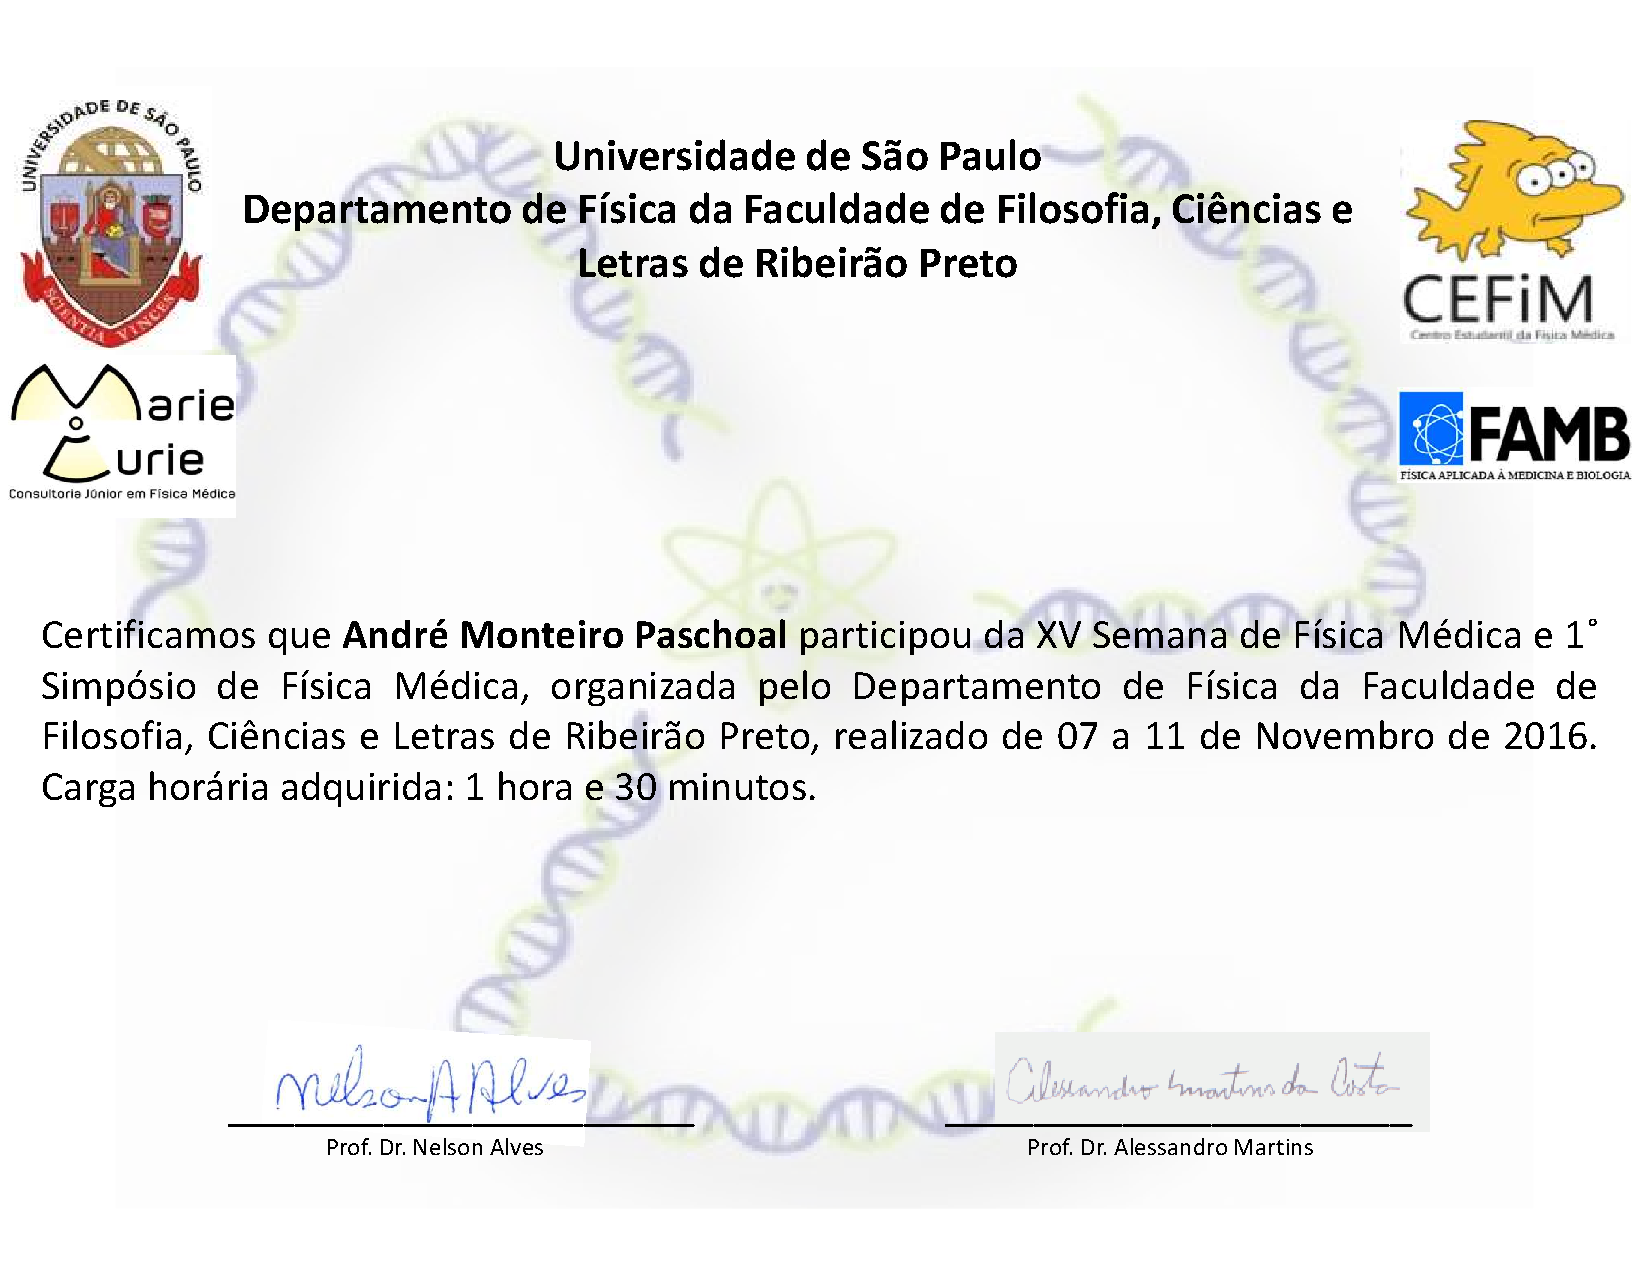
\includepdf[pages=-, scale=1,pagecommand=\thispagestyle{empty}]{\detokenize{Diplomas/certificadoSFM2016}}

\newpage
\subsection{Participa\c{c}\~{a}o em Eventos Cient\'{\i}ficos (com apresenta\c{c}\~{a}o de trabalho ou oferecimento de cursos, palestras ou debates}
\label{certificados:CBFM2017}
Esta subseção apresenta o comprovante da participação no XXII Congresso Brasileiro de Física Médica com seus respectivos propósitos.
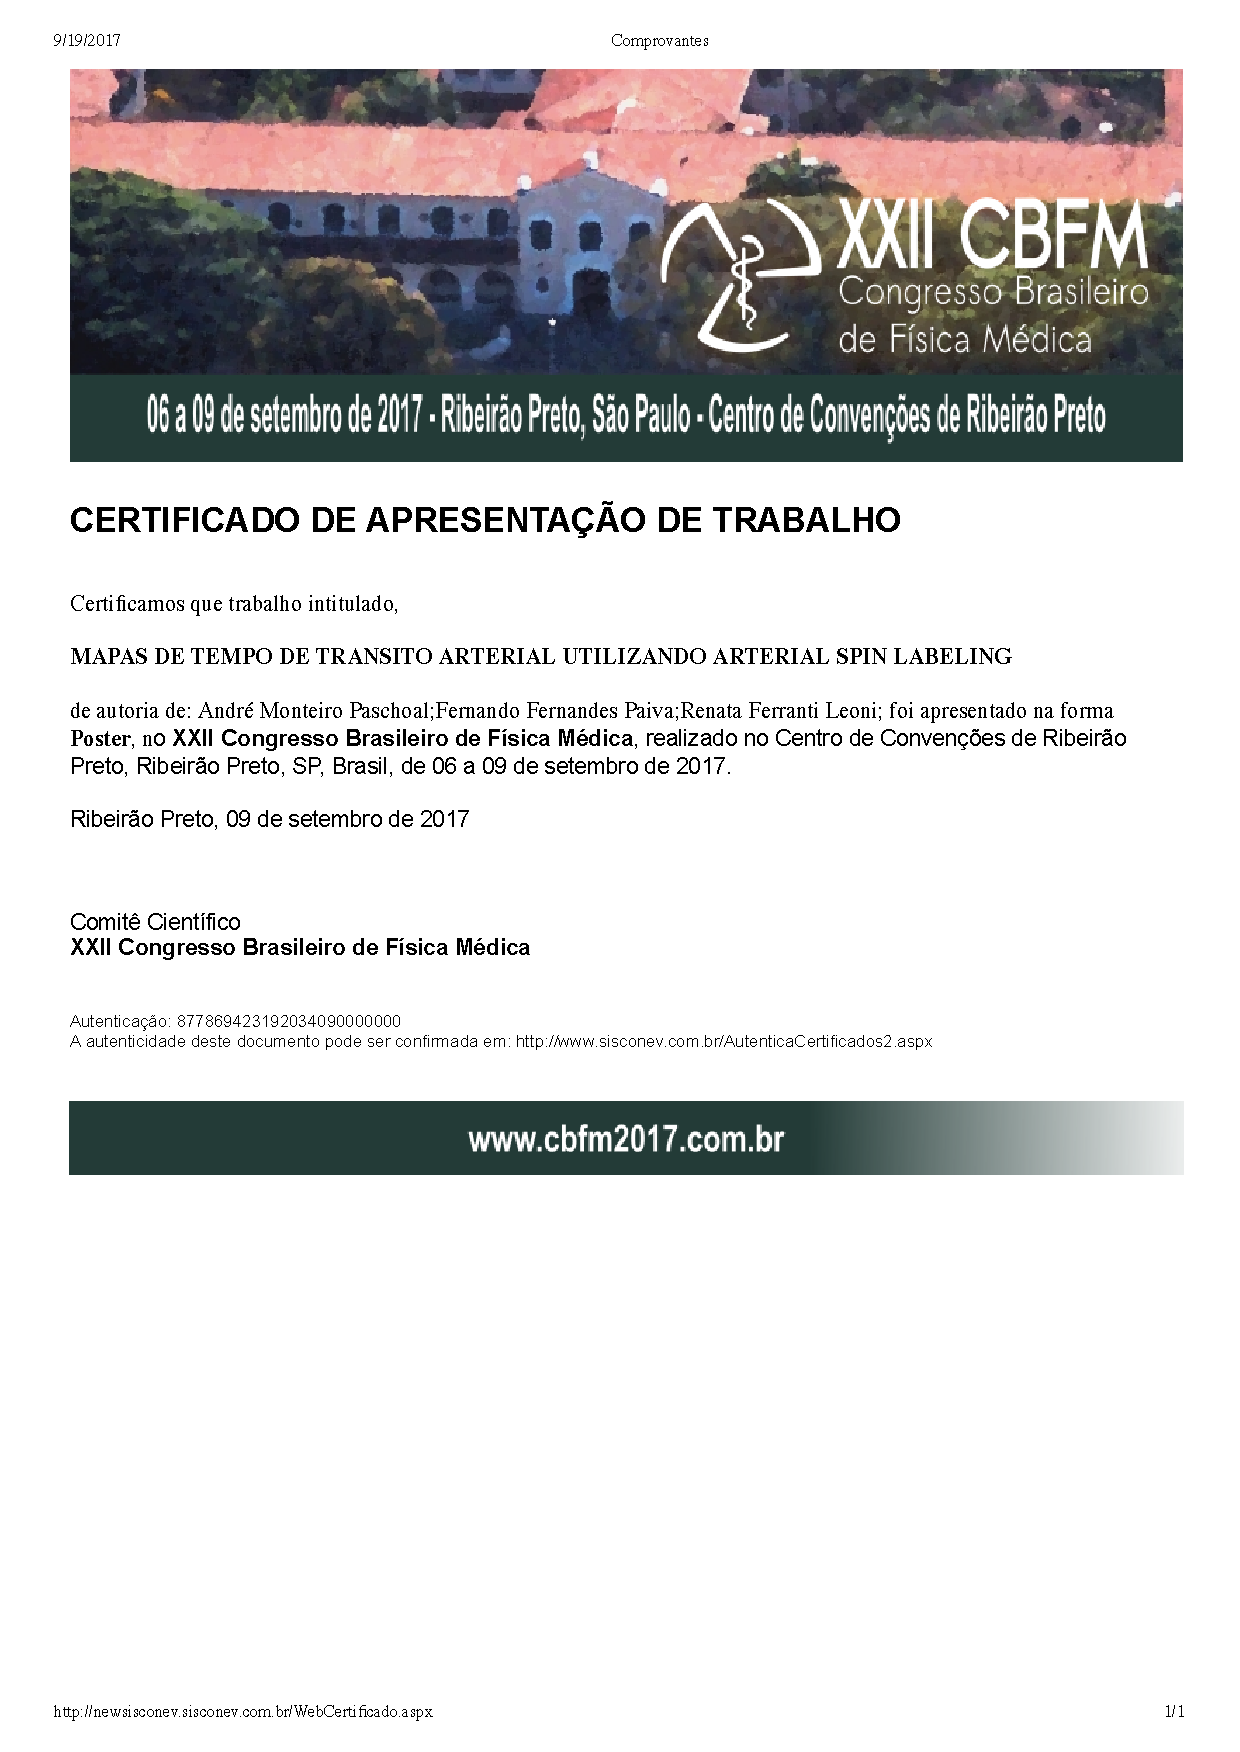
\includepdf[pages=-, scale=1,pagecommand=\thispagestyle{empty}]{\detokenize{Diplomas/certificadoCBFM2017}}

\newpage
\subsection{Participa\c{c}\~{a}o em Eventos Cient\'{\i}ficos (com apresenta\c{c}\~{a}o de trabalho ou oferecimento de cursos, palestras ou debates}
\label{certificados:FAMB2017}
Esta subseção apresenta o comprovante da participação no Seminário semanal do programa de Física Aplicada à Medicina e Biologia com seus respectivos propósitos.
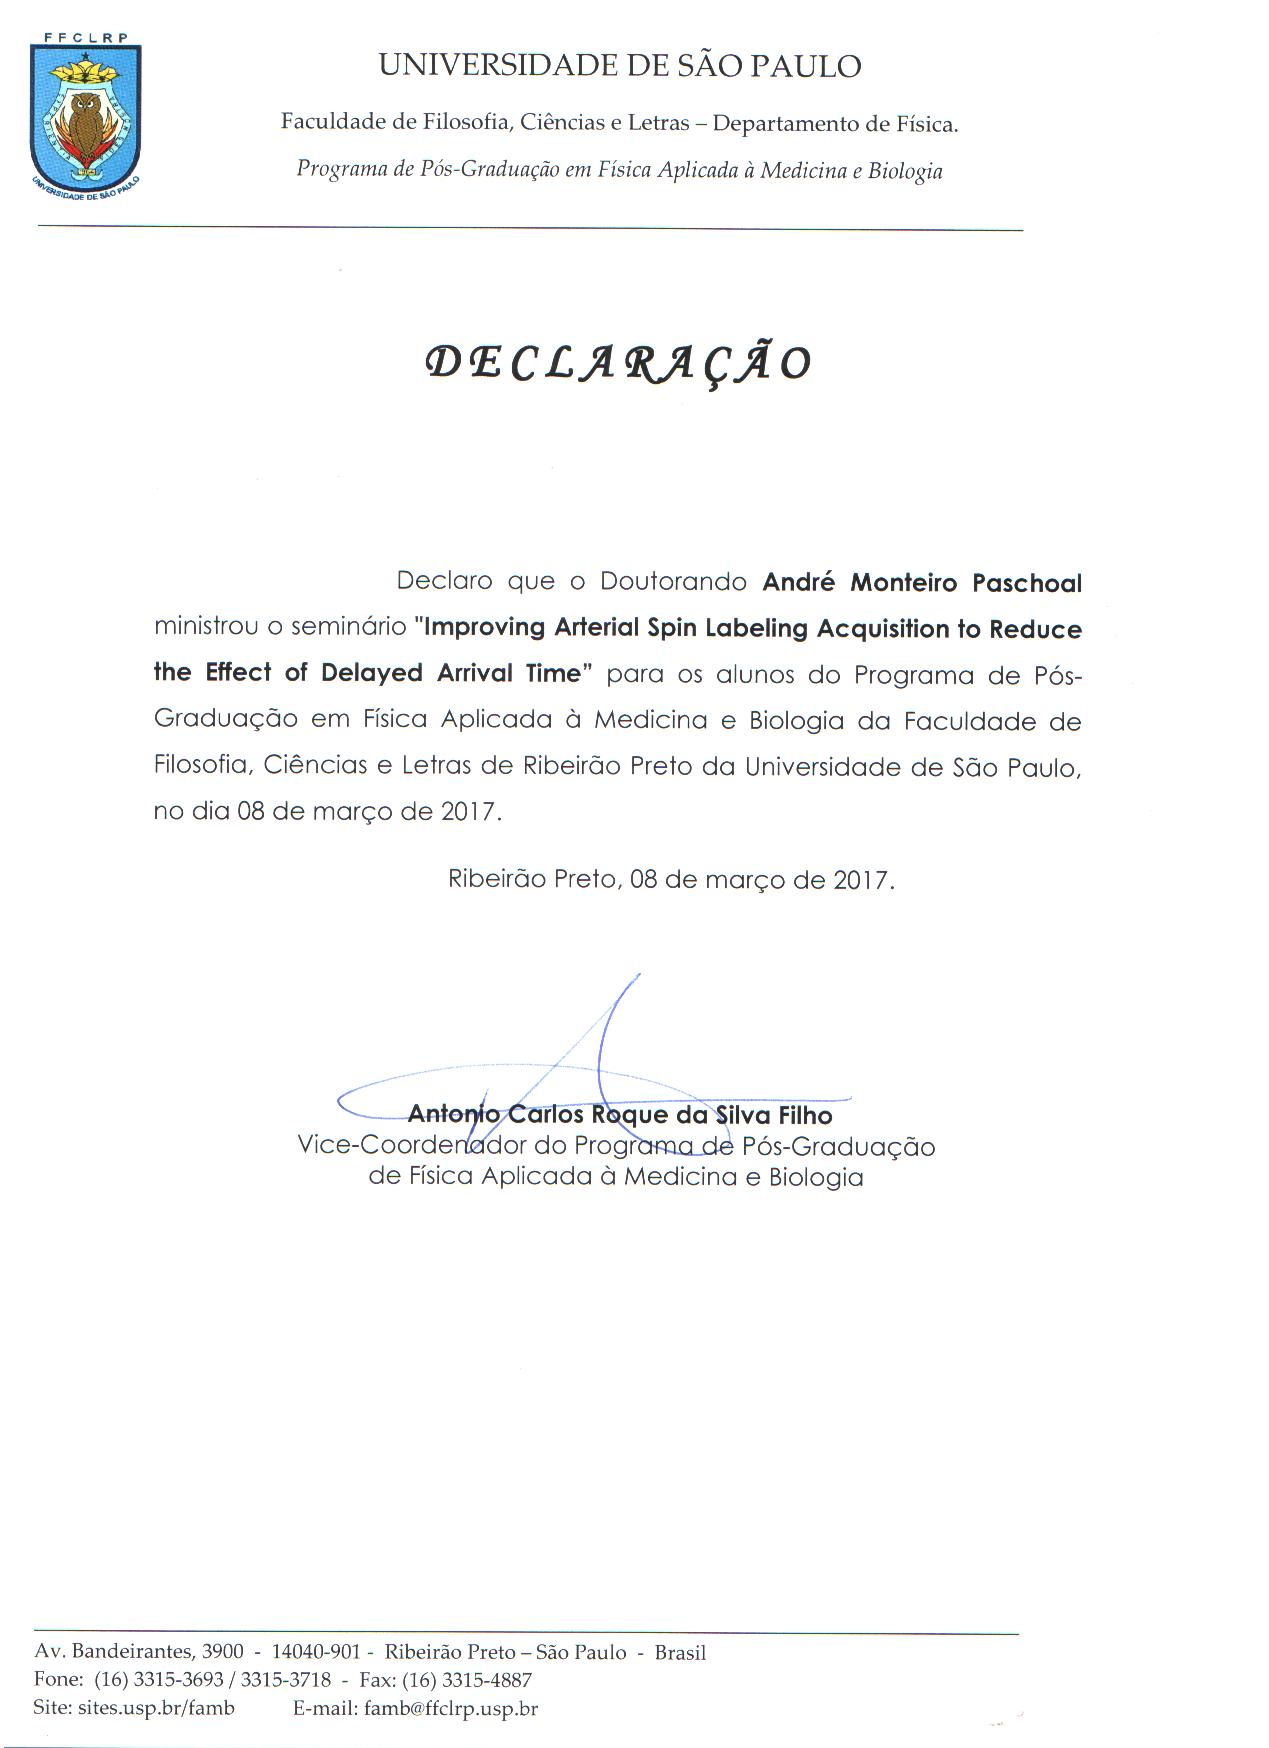
\includepdf[pages=-, scale=1,pagecommand=\thispagestyle{empty}]{\detokenize{Diplomas/CertificadoApresentacaoSeminarioFAMB}}

\newpage
\subsection{Participa\c{c}\~{a}o em Eventos Cient\'{\i}ficos (com apresenta\c{c}\~{a}o de trabalho ou oferecimento de cursos, palestras ou debates}
\label{certificados:Neuromat}
Esta subseção apresenta o comprovante da participação na palestra ``O Cérebro estatístico: desafios científicos do CEPID NeuroMat'' com seus respectivos propósitos.
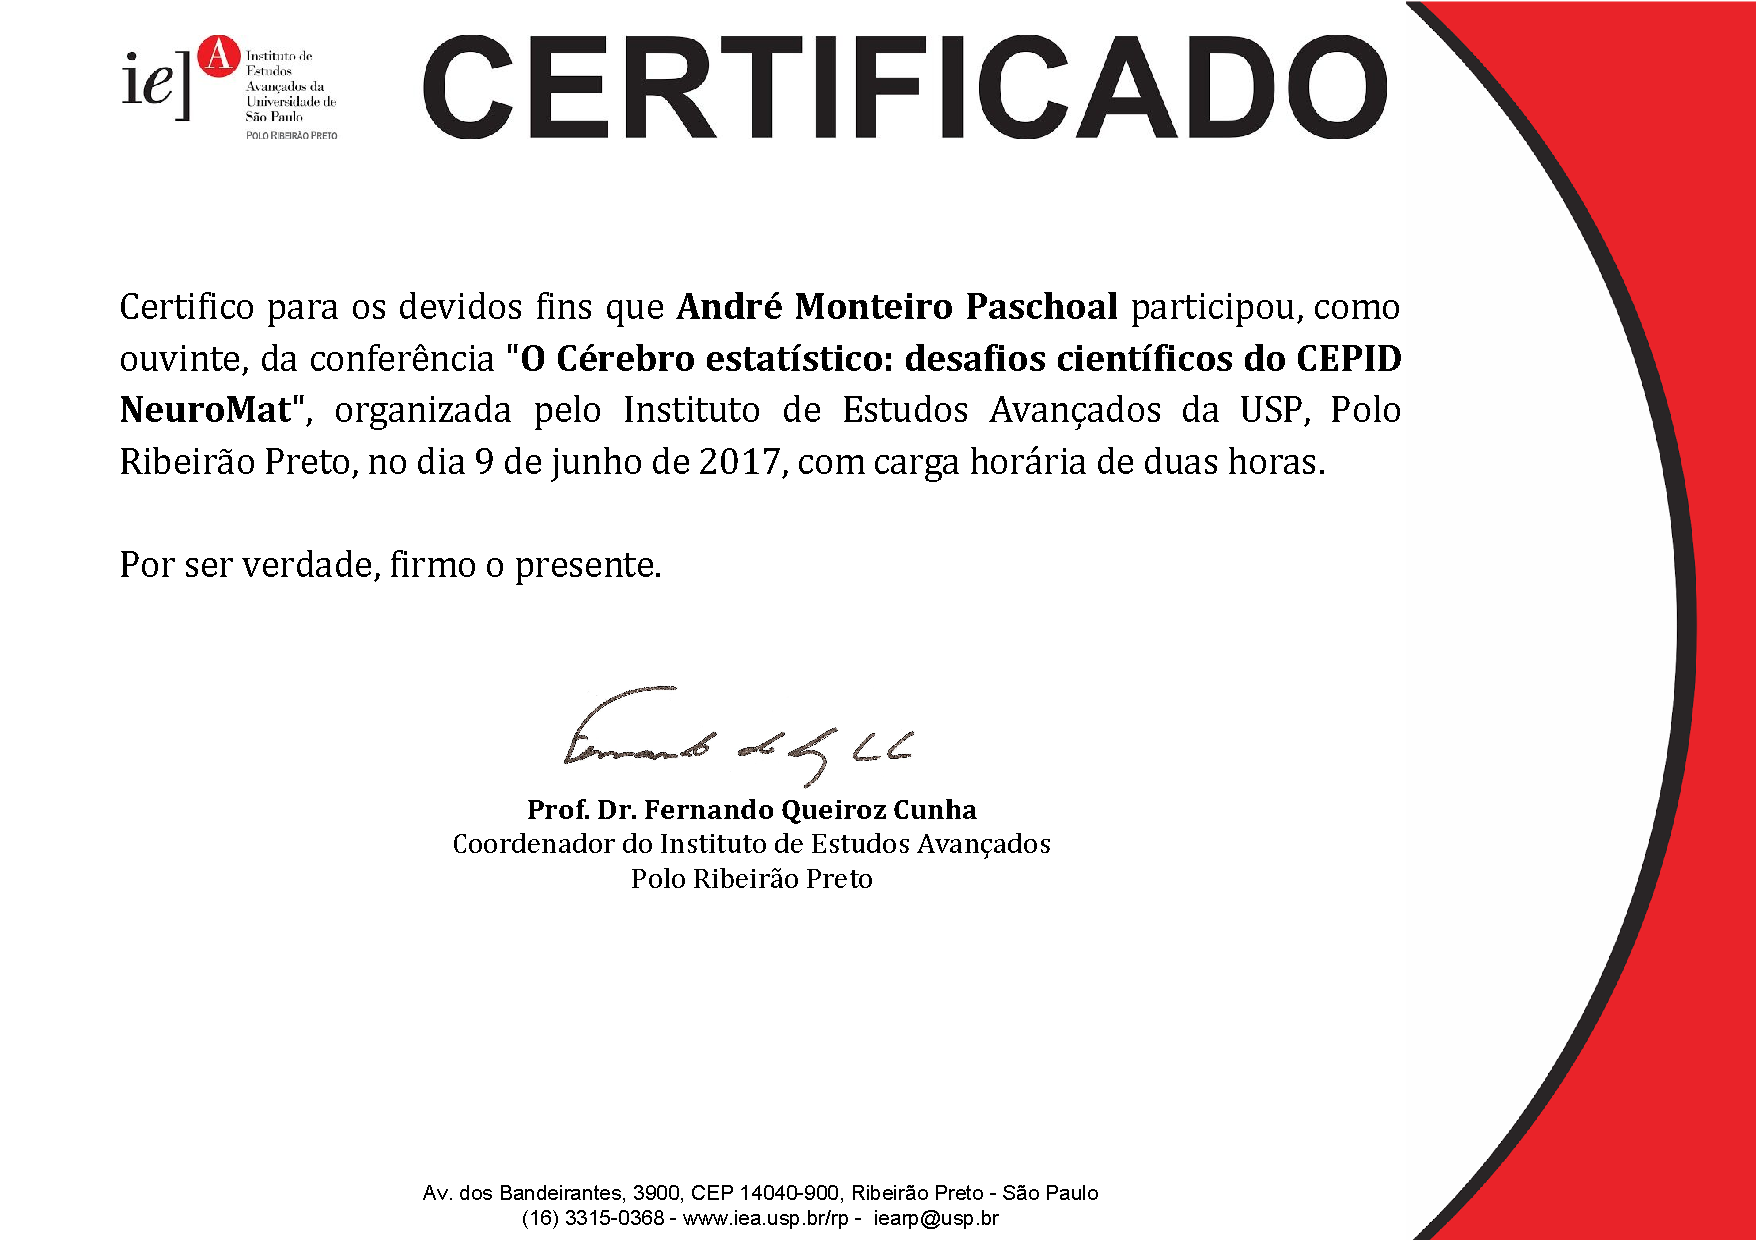
\includepdf[pages=-, scale=1,pagecommand=\thispagestyle{empty}]{\detokenize{Diplomas/Neutomat_06_2017}}

\newpage
\subsection{Participa\c{c}\~{a}o em Eventos Cient\'{\i}ficos (com apresenta\c{c}\~{a}o de trabalho ou oferecimento de cursos, palestras ou debates}
\label{certificados:SIIM2017}
Esta subseção apresenta o comprovante da participação no  8º Simpósio de Instrumentação e Imagens Médicas (SIIM) e 7º Simpósio de Processamento de Sinais (SPS) com seus respectivos propósitos.
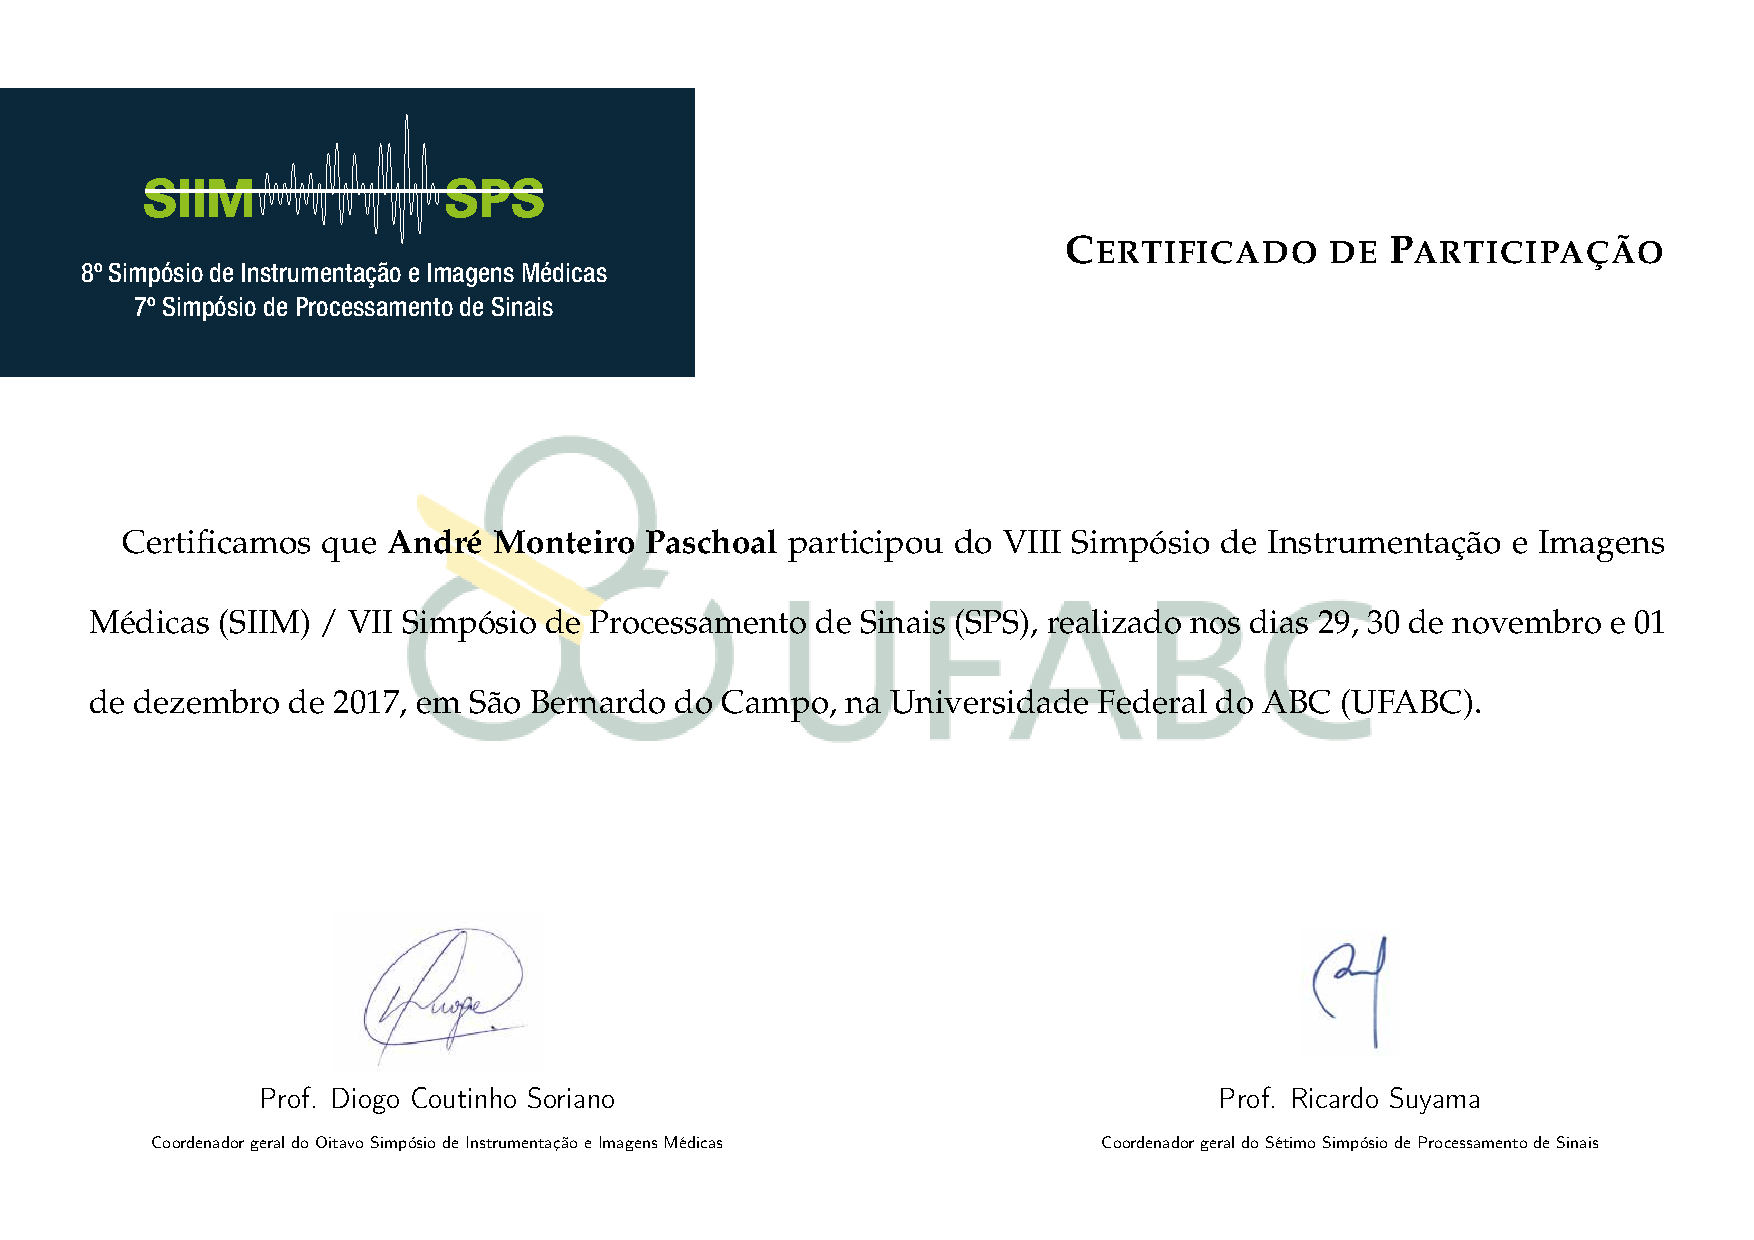
\includepdf[pages=-, scale=1,pagecommand=\thispagestyle{empty}]{\detokenize{Diplomas/SIIM2017}}

\newpage
\subsection{Participa\c{c}\~{a}o em Eventos Cient\'{\i}ficos (com apresenta\c{c}\~{a}o de trabalho ou oferecimento de cursos, palestras ou debates}
\label{certificados:ISMRM2017}
Esta subseção apresenta o comprovante da participação no 
ISMRM 25th Annual Meeting \& Exhibition com seus respectivos propósitos. \\
Obs: Ese congresso não emite certificado de apresentação de trabalhos, apenas de participação no evento.
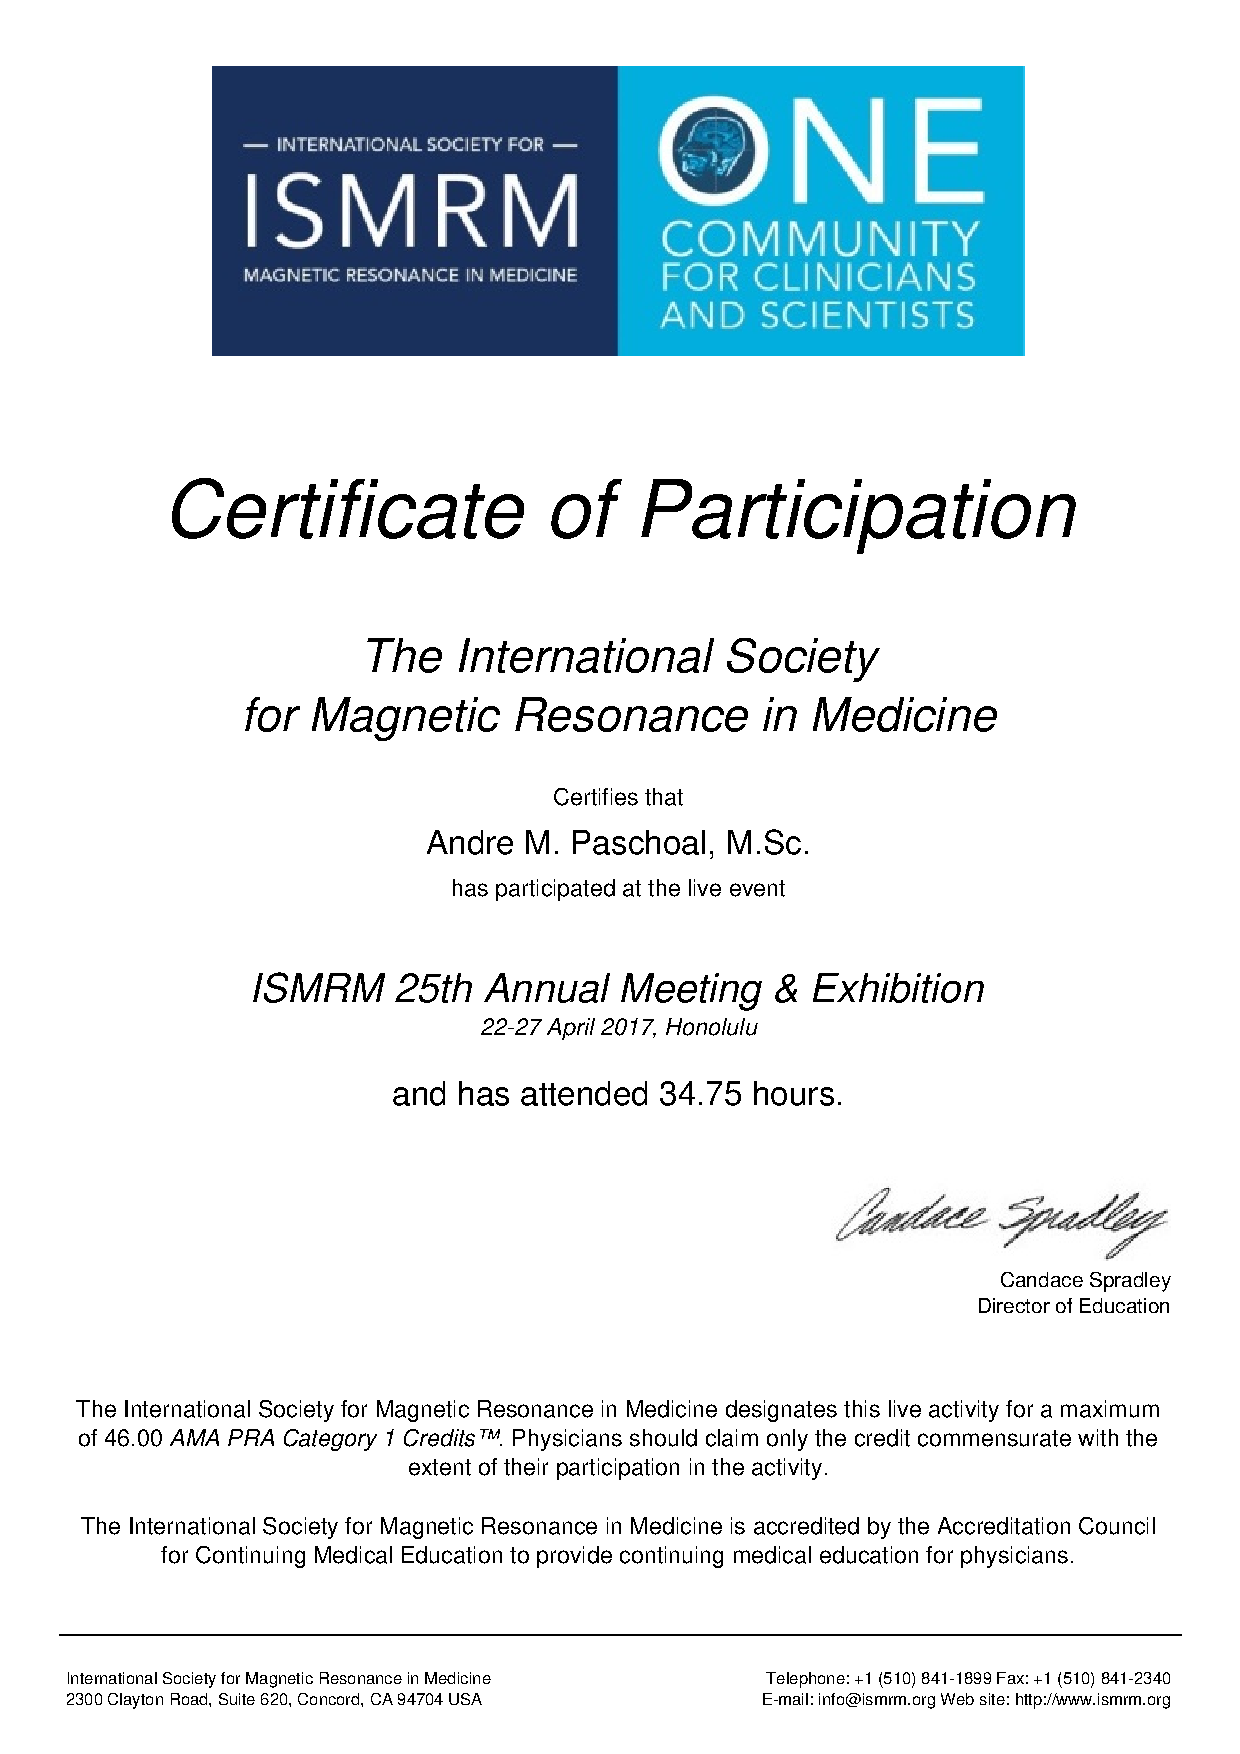
\includepdf[pages=-, scale=1,pagecommand=\thispagestyle{empty}]{\detokenize{Diplomas/ISMRM2017}}
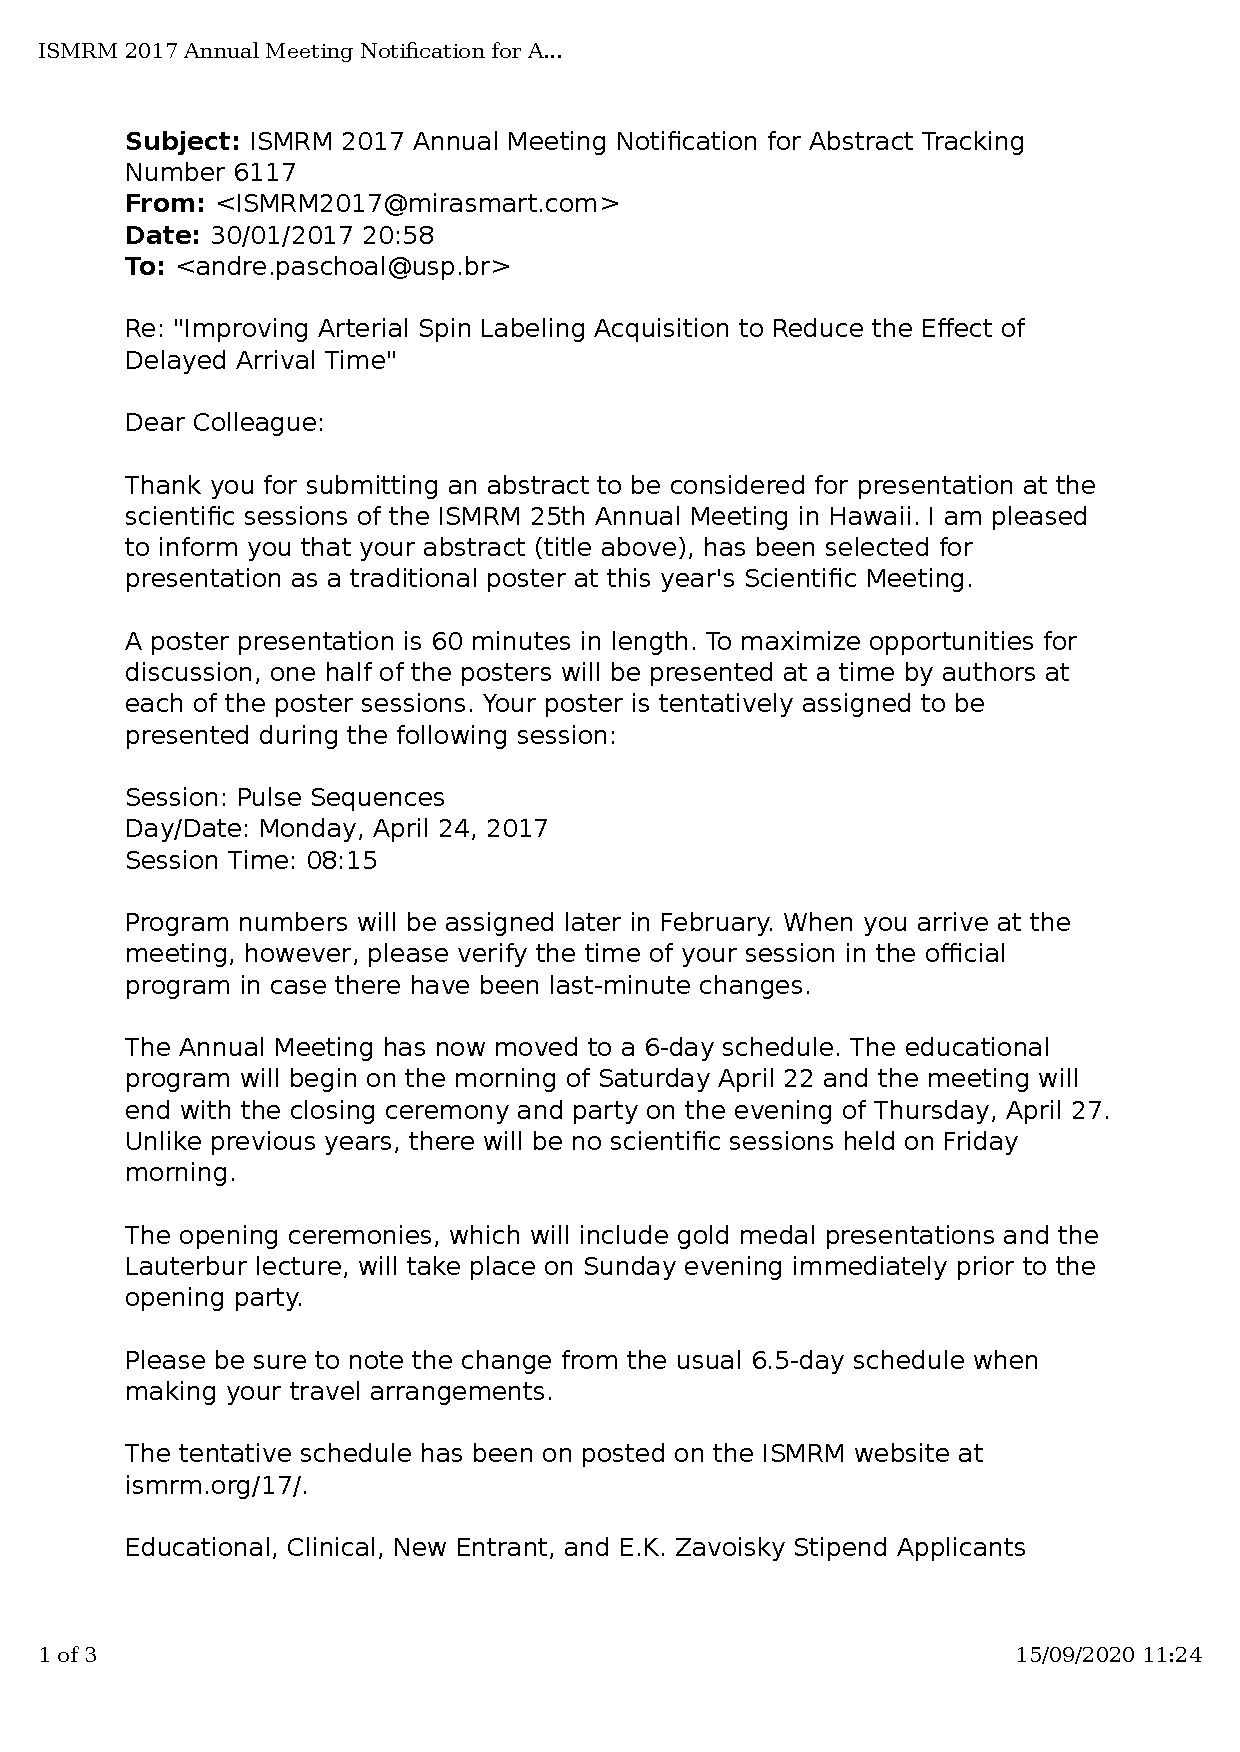
\includepdf[pages=-, scale=1,pagecommand=\thispagestyle{empty}]{\detokenize{Diplomas/AcceptanceISMRM2017}}

\newpage
\subsection{Participa\c{c}\~{a}o em Eventos Cient\'{\i}ficos (com apresenta\c{c}\~{a}o de trabalho ou oferecimento de cursos, palestras ou debates}
\label{certificados:BRAINN2017}
Esta subseção apresenta o comprovante da participação no 4º BRAINN Congress com seus respectivos propósitos.
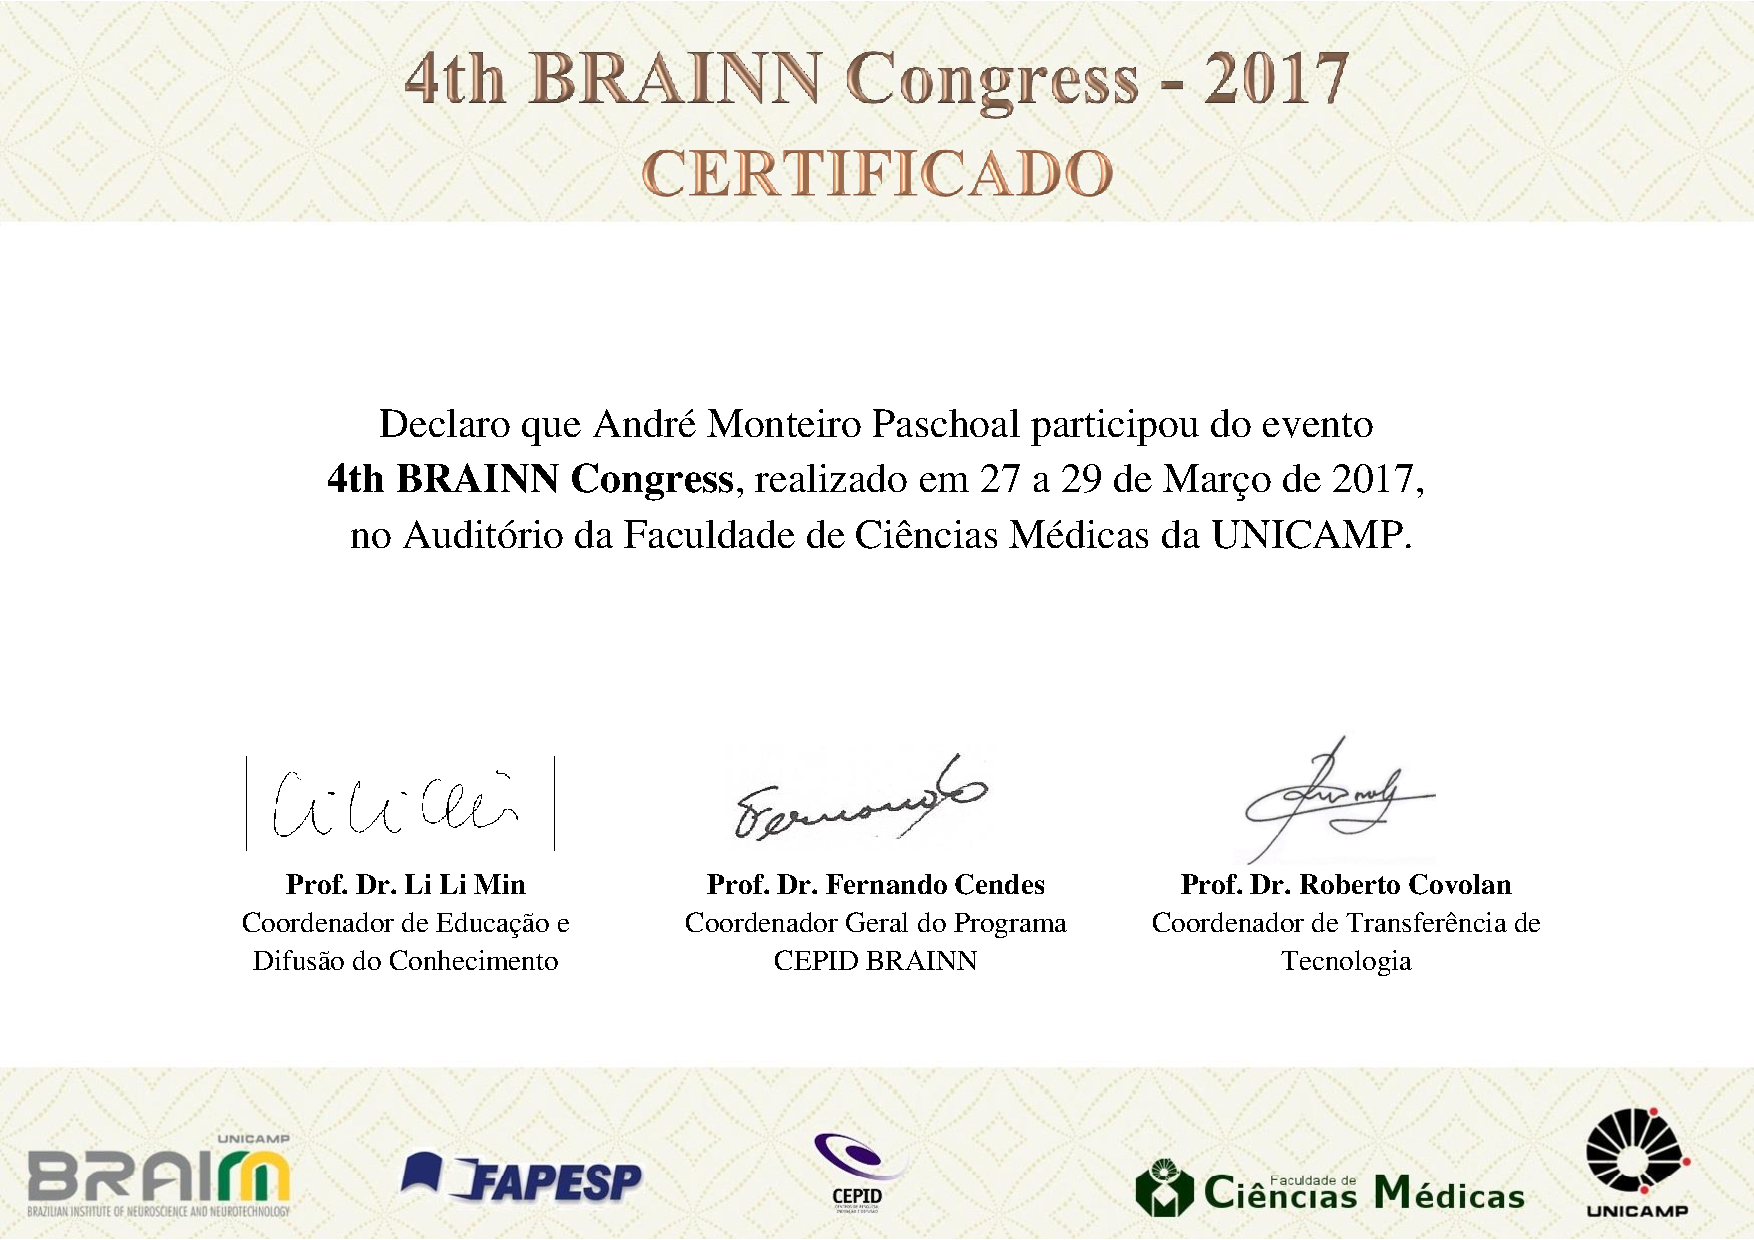
\includepdf[pages=-, scale=1,pagecommand=\thispagestyle{empty}]{\detokenize{Diplomas/BRAINN2017}}

\newpage
\subsection{Participa\c{c}\~{a}o em Eventos Cient\'{\i}ficos (com apresenta\c{c}\~{a}o de trabalho ou oferecimento de cursos, palestras ou debates}
\label{certificados:BRAINN2018}
Esta subseção apresenta o comprovante da participação no 5º BRAINN Congress com seus respectivos propósitos.
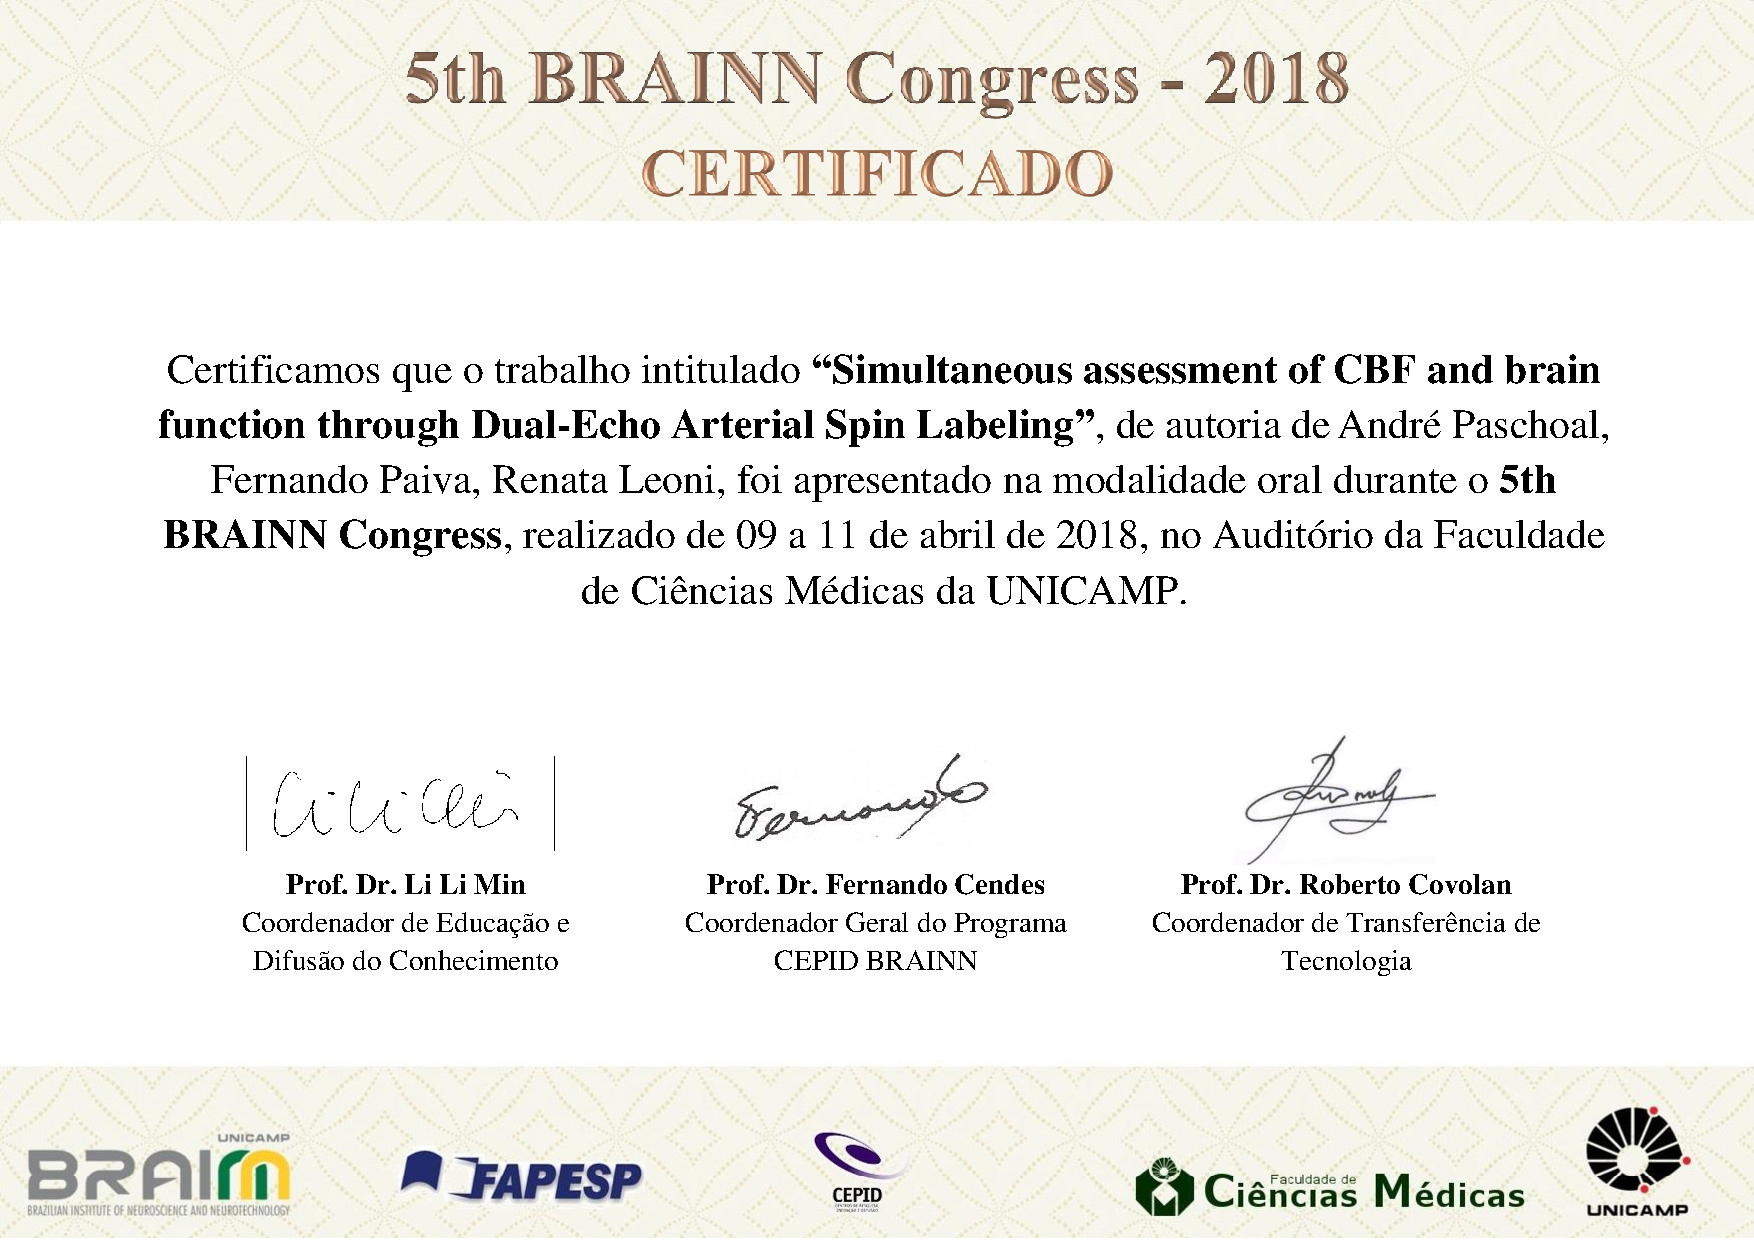
\includepdf[pages=-, scale=1,pagecommand=\thispagestyle{empty}]{\detokenize{Diplomas/BRAINN2018_apresentacao}}

\newpage
\subsection{Participa\c{c}\~{a}o em Eventos Cient\'{\i}ficos (com apresenta\c{c}\~{a}o de trabalho ou oferecimento de cursos, palestras ou debates}
\label{certificados:BRAINN2018_2}
Esta subseção apresenta o resumo publicado nos anais do 5º BRAINN Congress com seus respectivos propósitos.
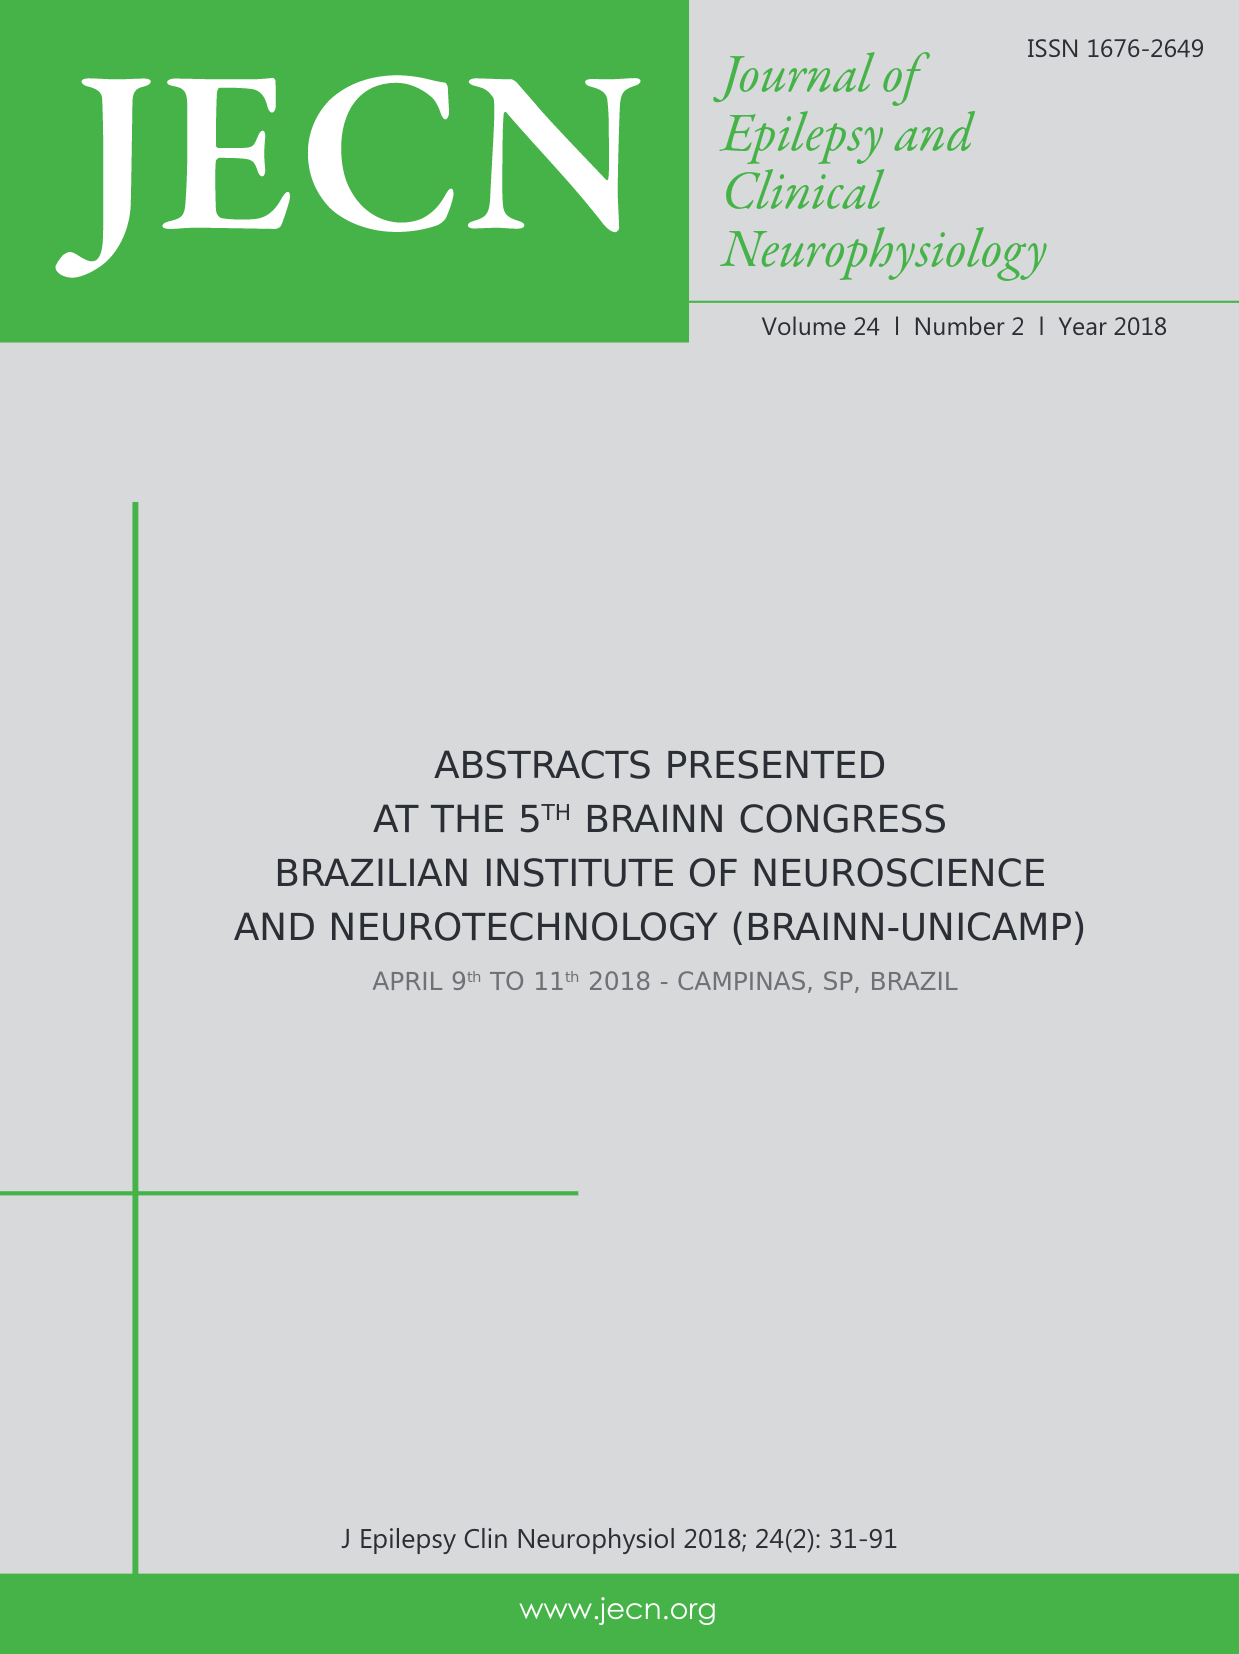
\includepdf[pages=-, scale=1,pagecommand=\thispagestyle{empty}]{\detokenize{docs/brainn2018}}

\newpage
\subsection{Participa\c{c}\~{a}o em Eventos Cient\'{\i}ficos (com apresenta\c{c}\~{a}o de trabalho ou oferecimento de cursos, palestras ou debates}
\label{certificados:ISMRM2018}
Esta subseção apresenta o comprovante da participação no Joint Annual Meeting ISMRM-ESMRMB com seus respectivos propósitos. \\
Obs: Ese congresso não emite certificado de apresentação de trabalhos, apenas de participação no evento.
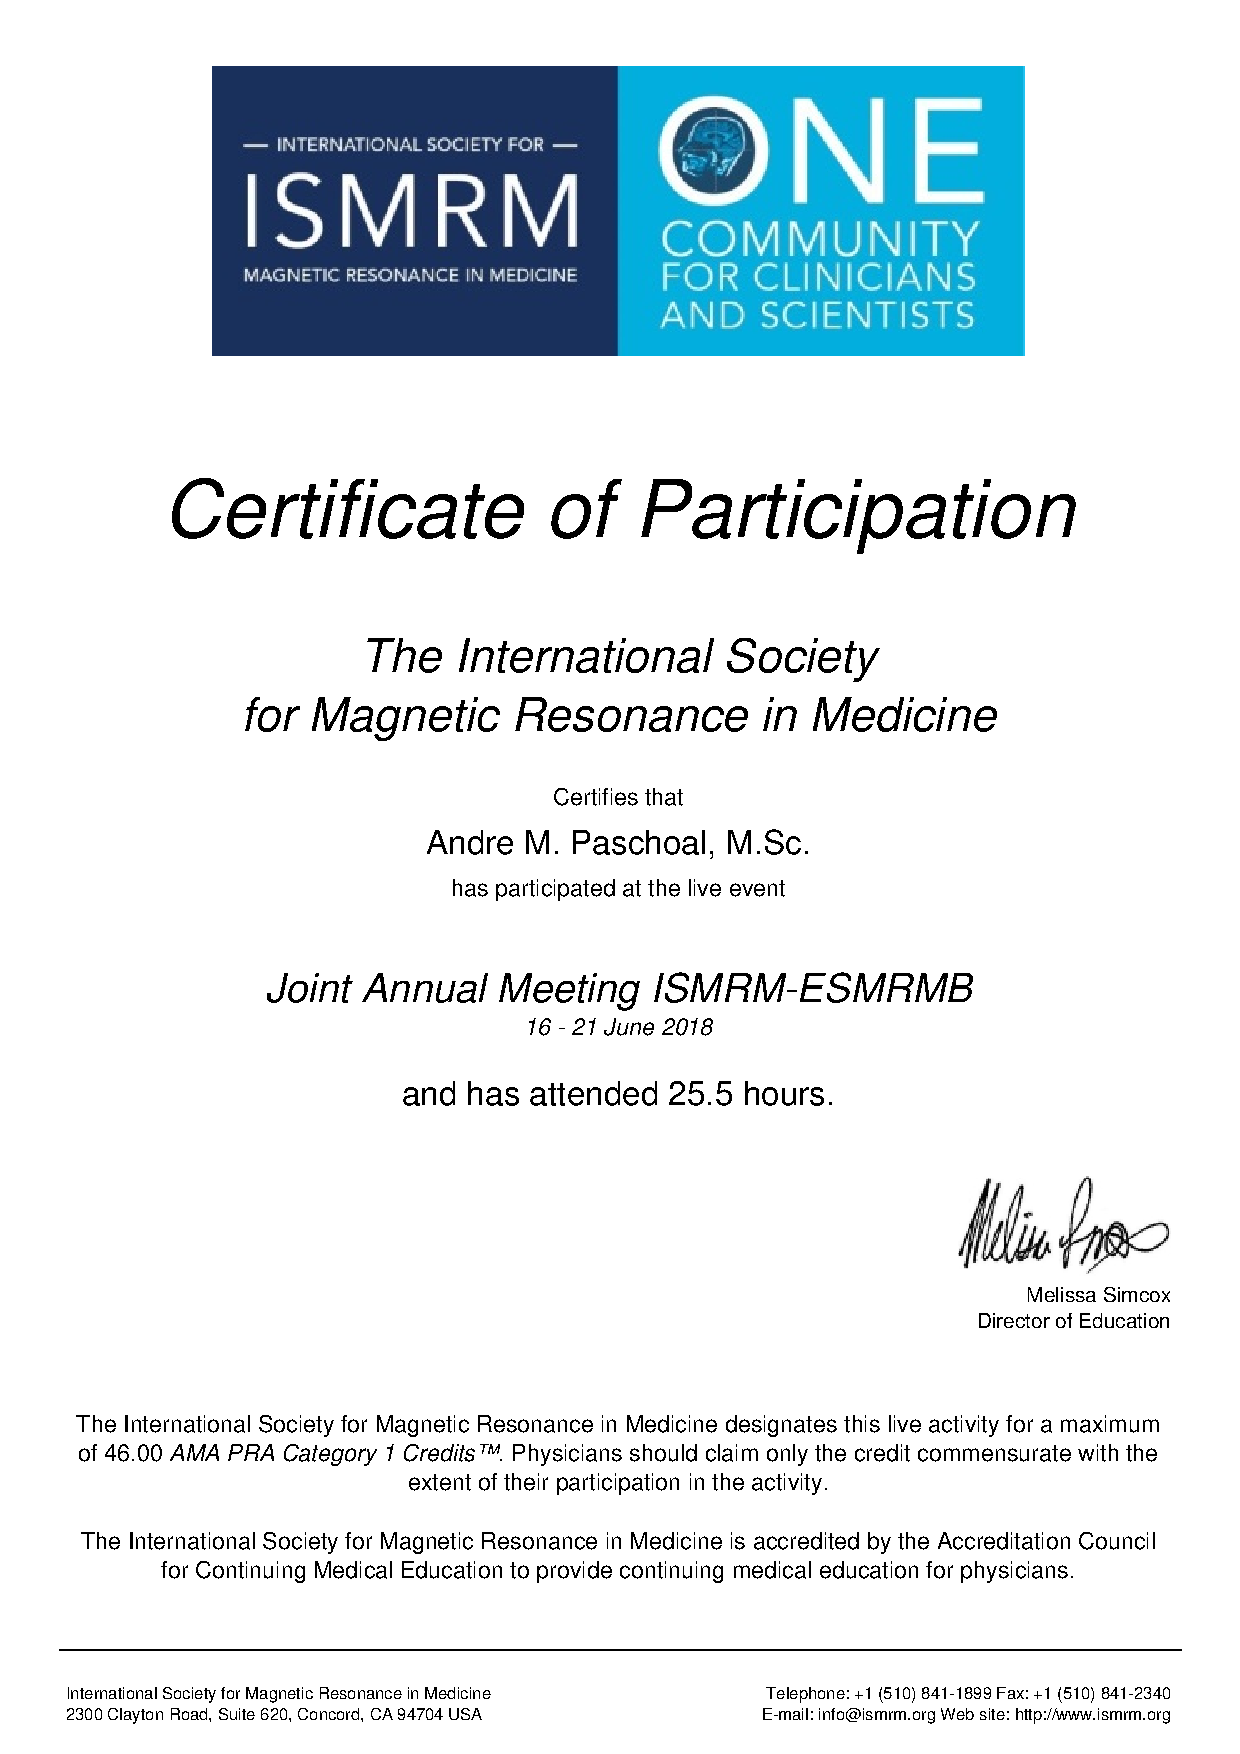
\includepdf[pages=-, scale=1,pagecommand=\thispagestyle{empty}]{\detokenize{Diplomas/ISMRM2018}}
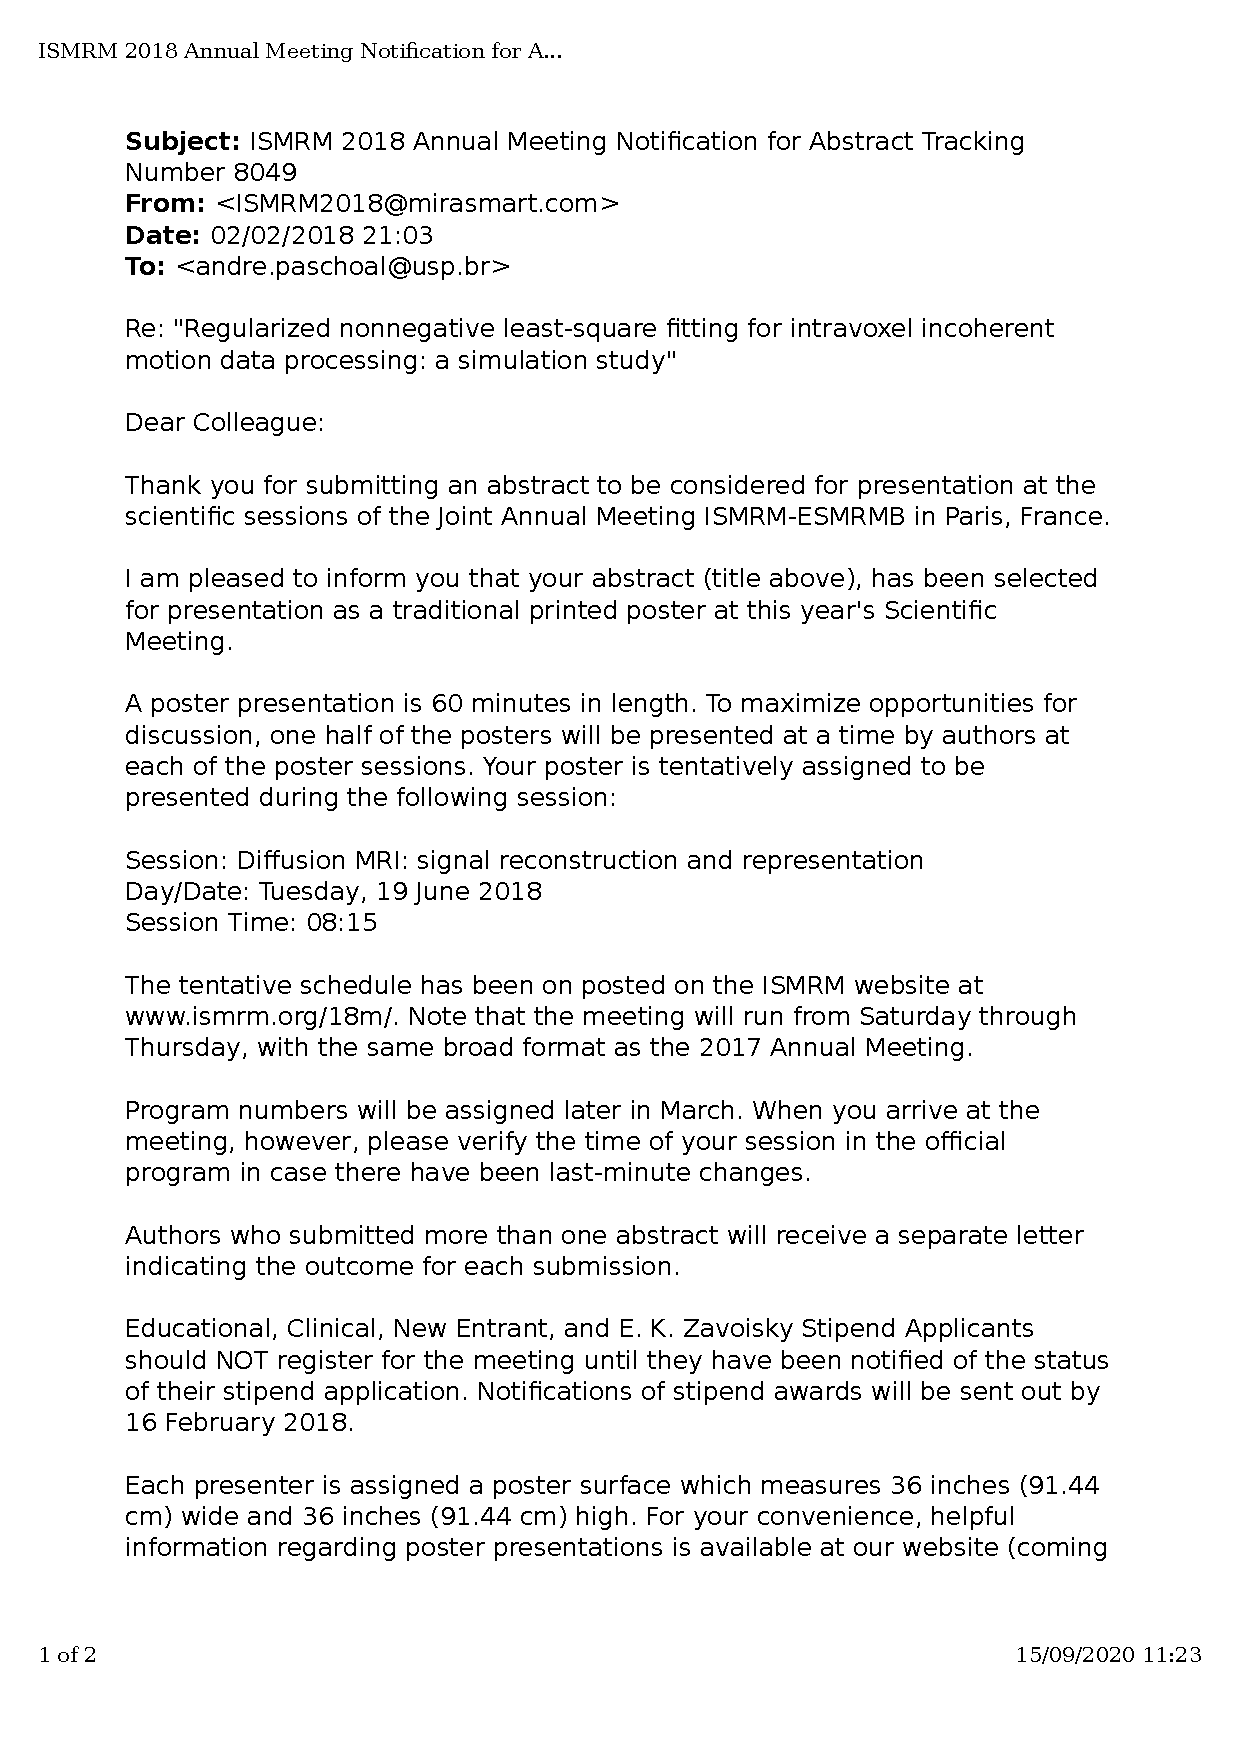
\includepdf[pages=-, scale=1,pagecommand=\thispagestyle{empty}]{\detokenize{Diplomas/AcceptanceISMRM2018_1}}
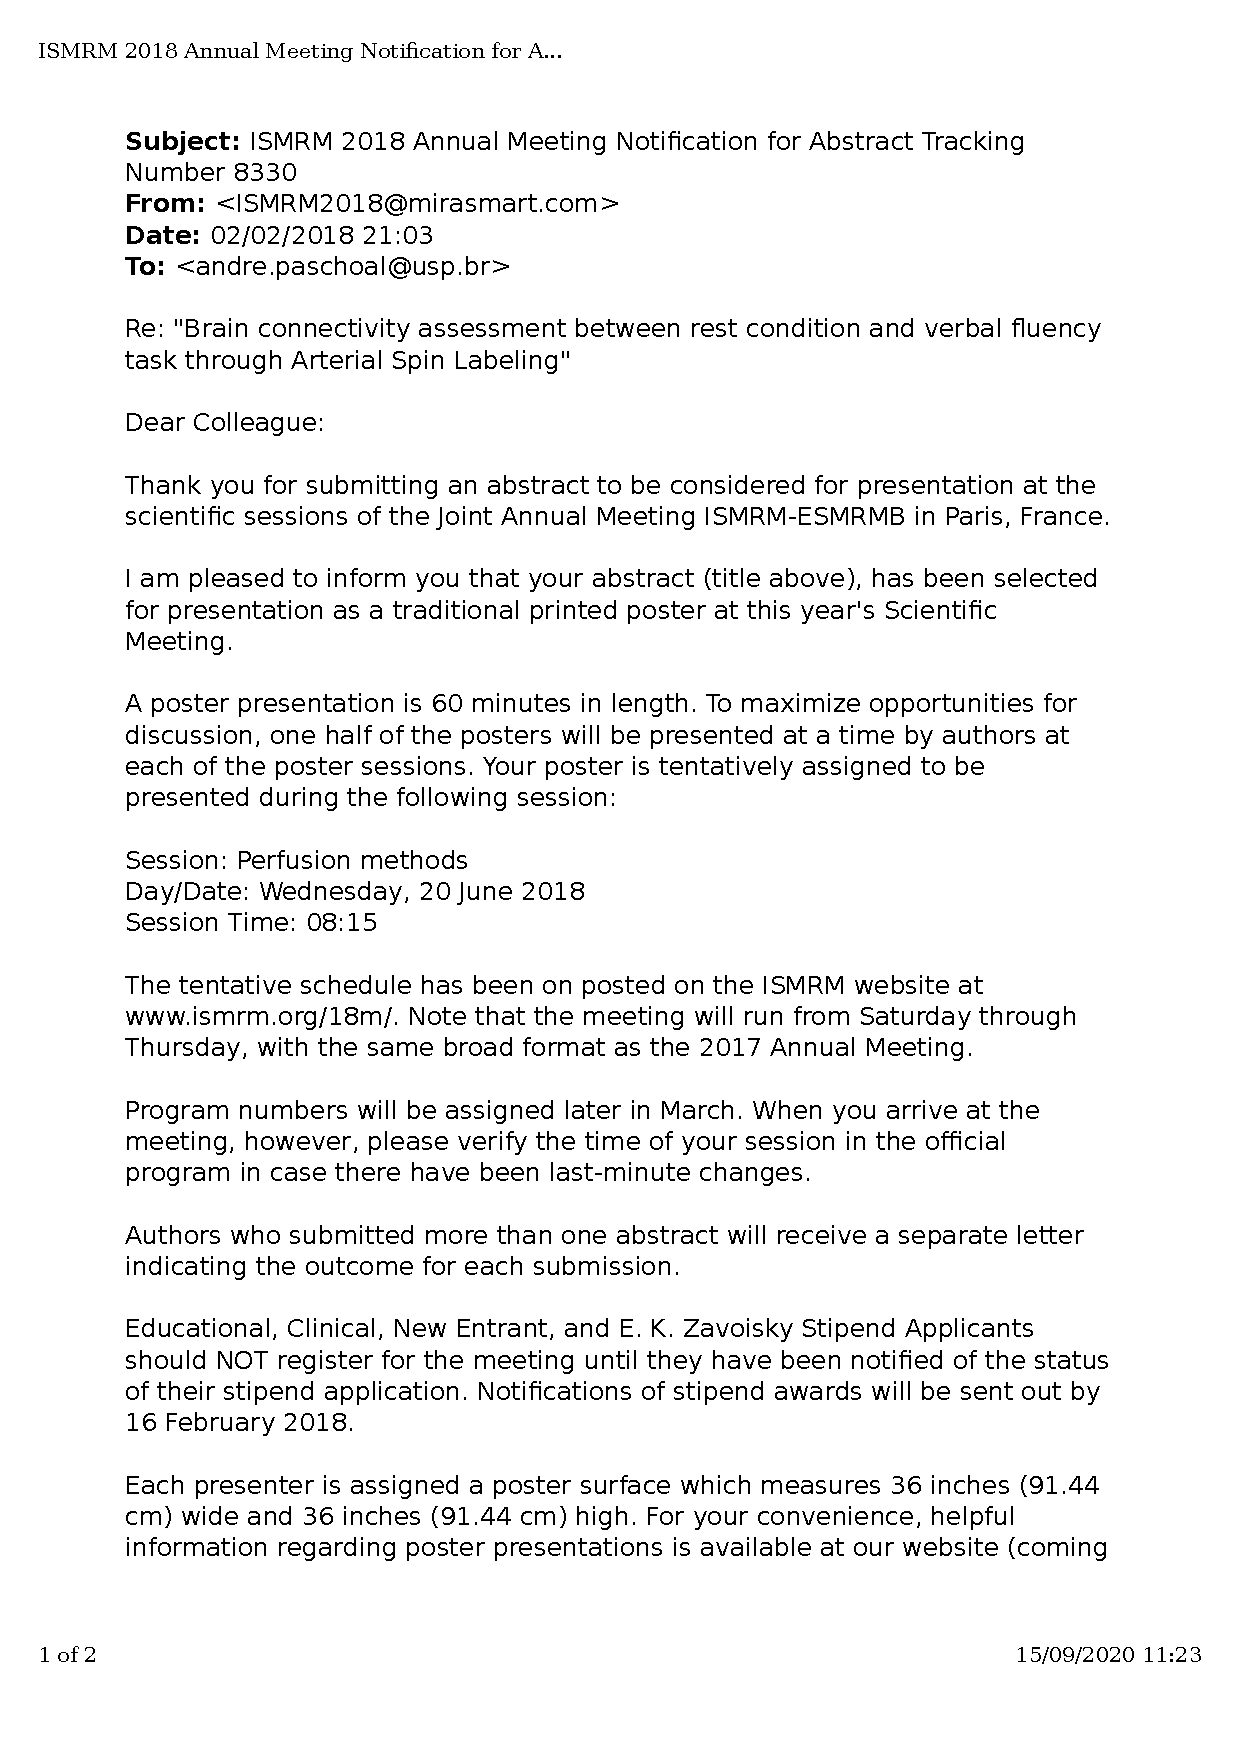
\includepdf[pages=-, scale=1,pagecommand=\thispagestyle{empty}]{\detokenize{Diplomas/AcceptanceISMRM2018_2}}


\newpage
\subsection{Participa\c{c}\~{a}o em Eventos Cient\'{\i}ficos (com apresenta\c{c}\~{a}o de trabalho ou oferecimento de cursos, palestras ou debates}
\label{certificados:SFM2017}
Esta subseção apresenta o comprovante da participação na XV Semana da Física Médica com seus respectivos propósitos.
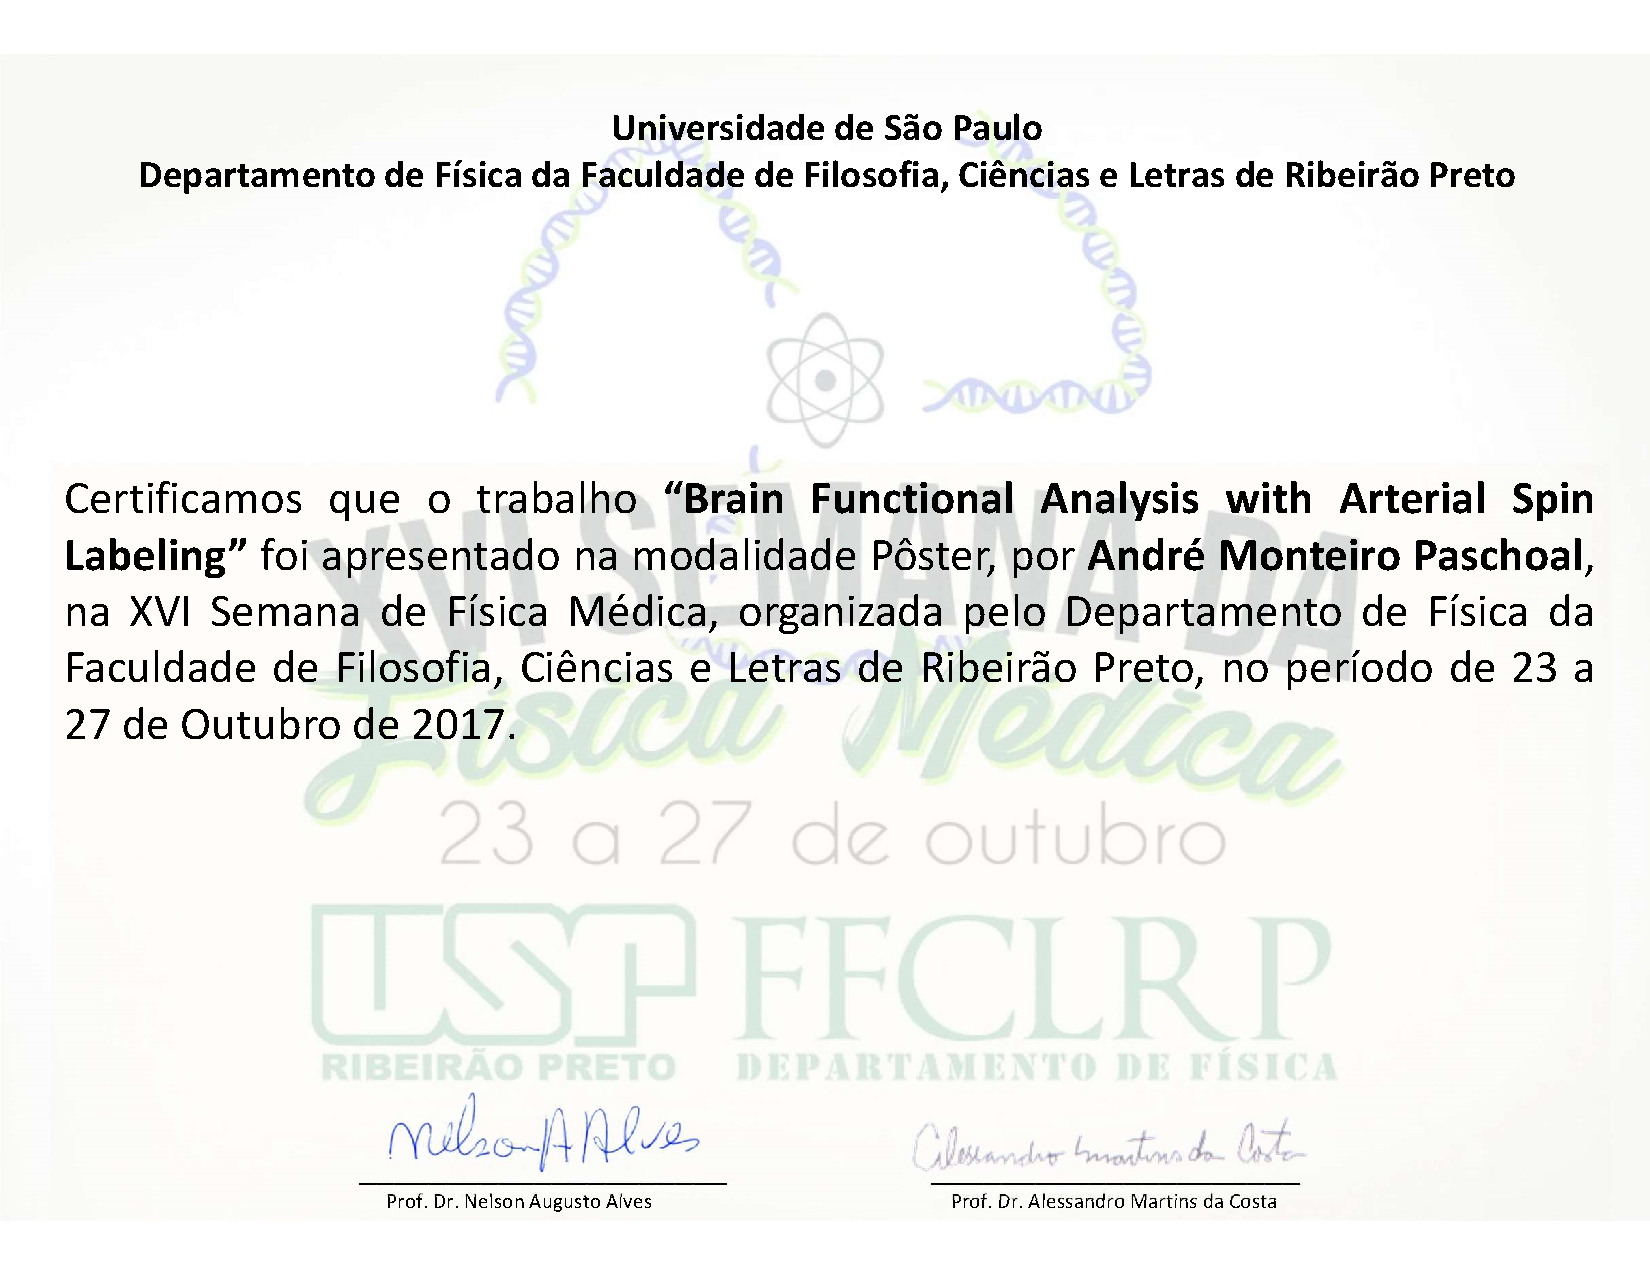
\includepdf[pages=-, scale=1,pagecommand=\thispagestyle{empty}]{\detokenize{Diplomas/SFM2017}}

\newpage
\subsection{Participa\c{c}\~{a}o em Eventos Cient\'{\i}ficos (com apresenta\c{c}\~{a}o de trabalho ou oferecimento de cursos, palestras ou debates}
\label{certificados:SFM2017_avaliador}
Esta subseção apresenta o comprovante da participação na XV Semana da Física Médica com seus respectivos propósitos.
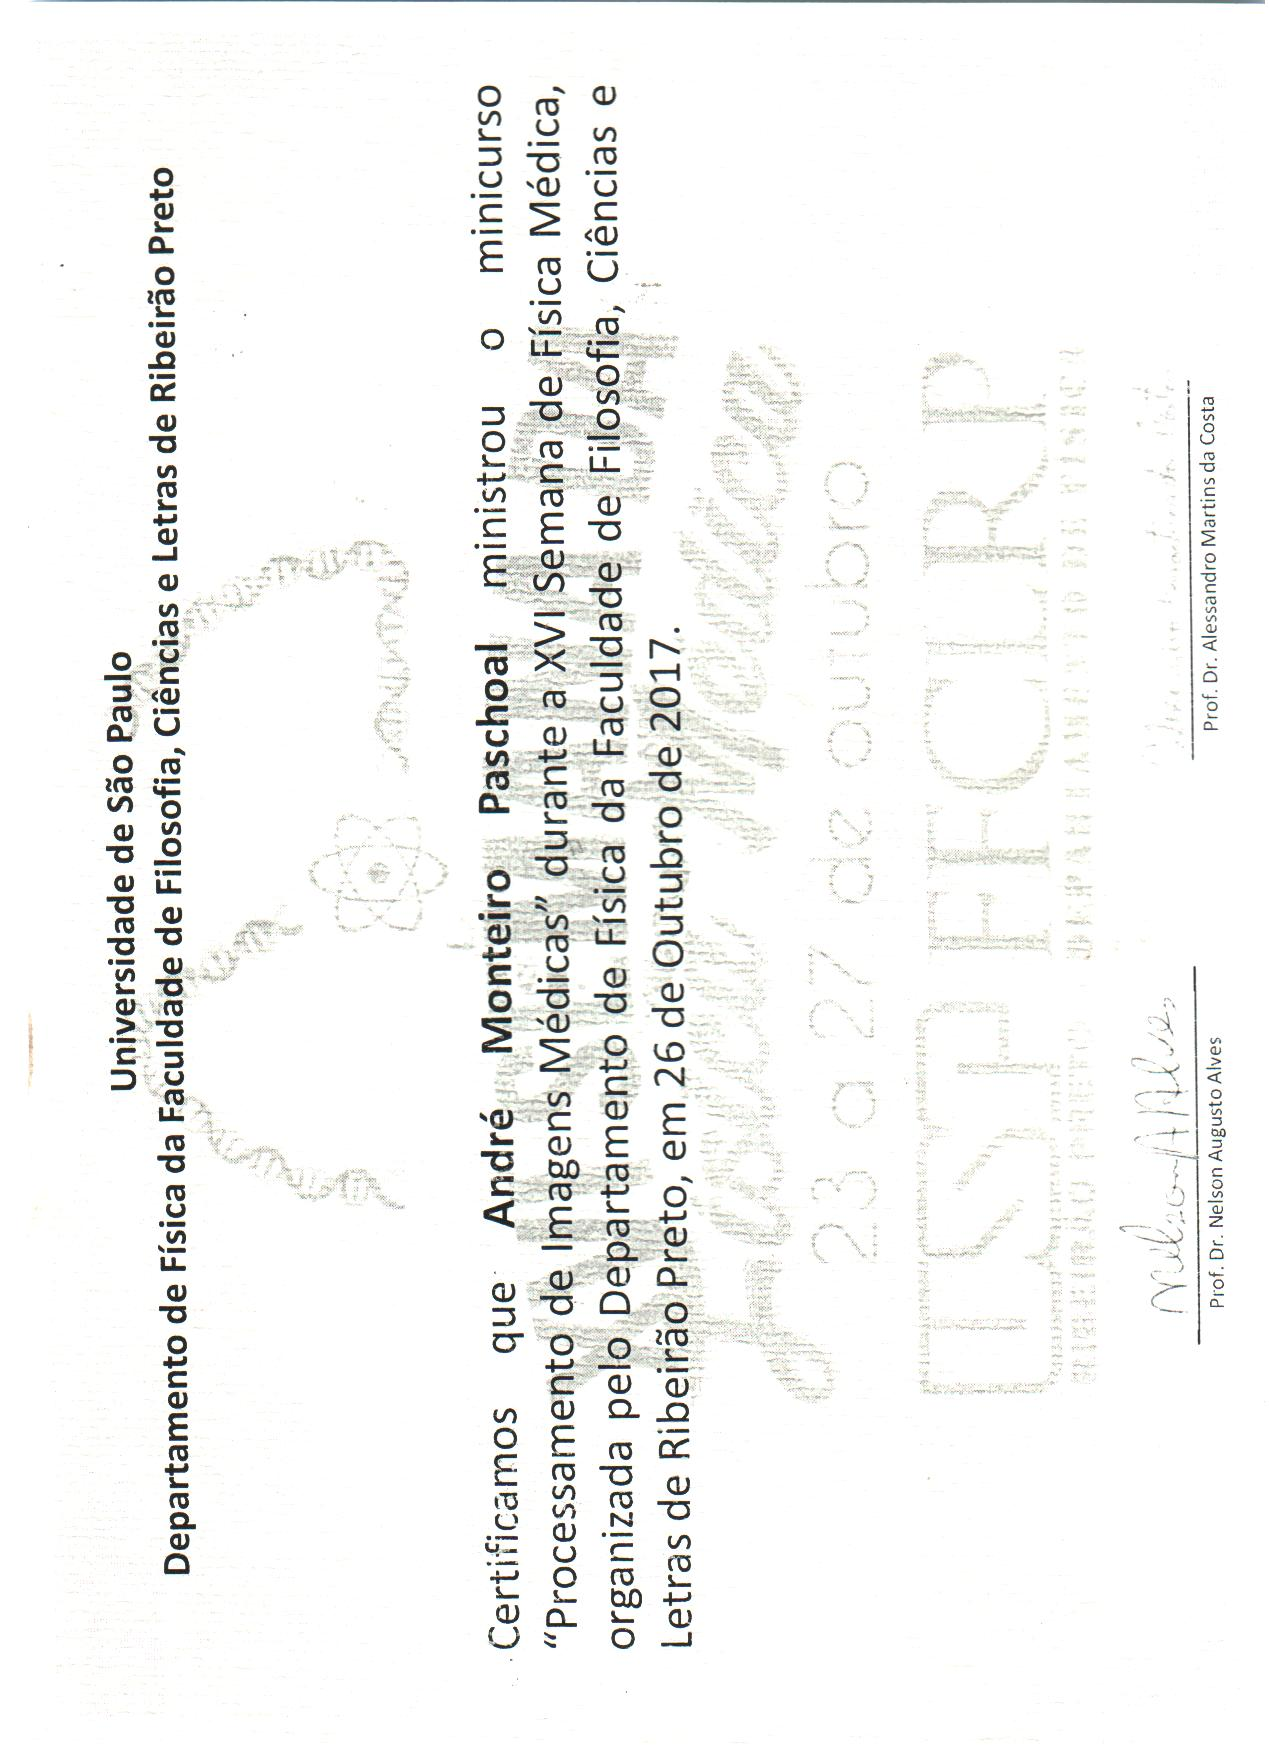
\includepdf[pages=-, scale=1,pagecommand=\thispagestyle{empty}]{\detokenize{Diplomas/CertificadoApresentacaoMiniCursoSFM}}

\newpage
\subsection{Participa\c{c}\~{a}o em Eventos Cient\'{\i}ficos (com apresenta\c{c}\~{a}o de trabalho ou oferecimento de cursos, palestras ou debates}
\label{certificados:SFM2018}
Esta subseção apresenta o comprovante da participação na XV Semana da Física Médica com seus respectivos propósitos.
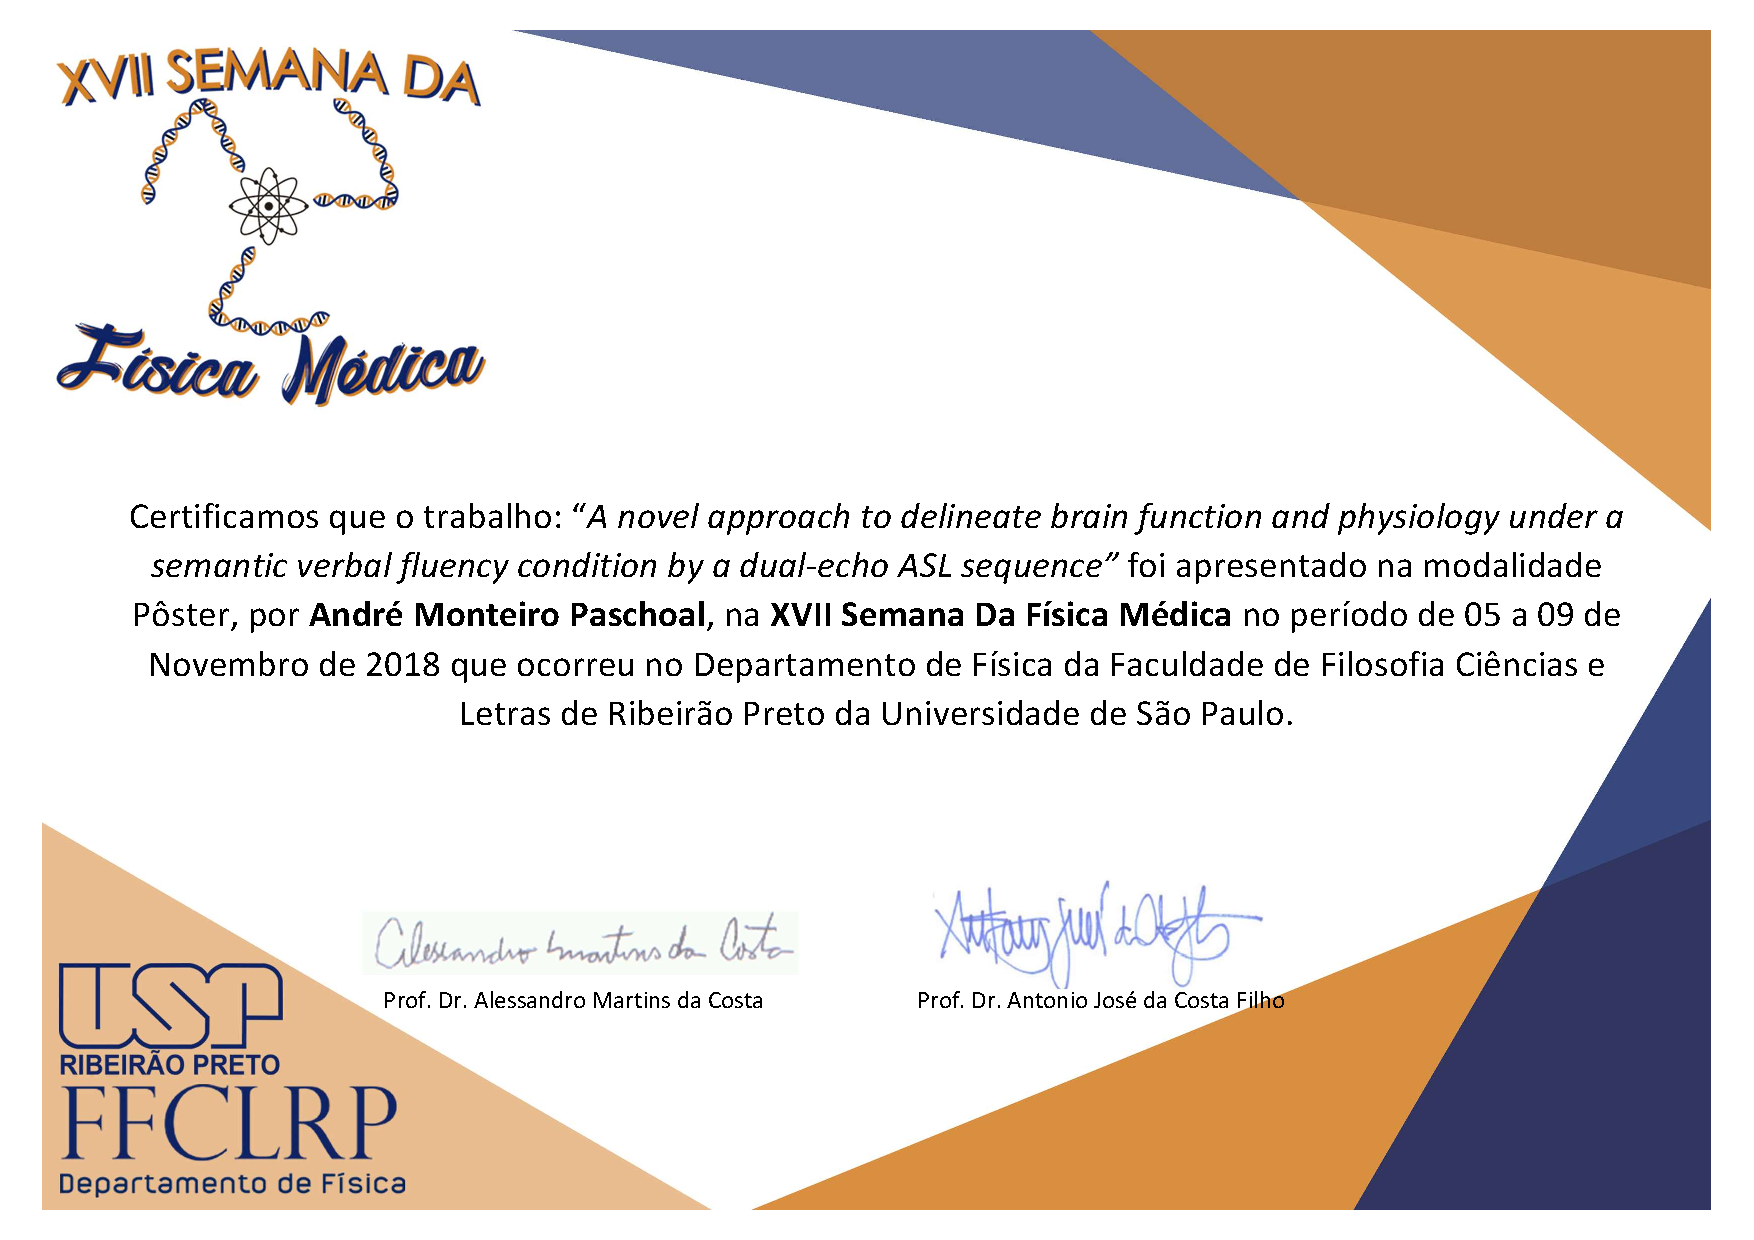
\includepdf[pages=-, scale=1,pagecommand=\thispagestyle{empty}]{\detokenize{Diplomas/SFM2018}}

\newpage
\subsection{Participa\c{c}\~{a}o em Eventos Cient\'{\i}ficos (com apresenta\c{c}\~{a}o de trabalho ou oferecimento de cursos, palestras ou debates}
\label{certificados:ISMRMBenelux}
Esta subseção apresenta o comprovante da participação no ISMRM Benelux Chapter com seus respectivos propósitos.
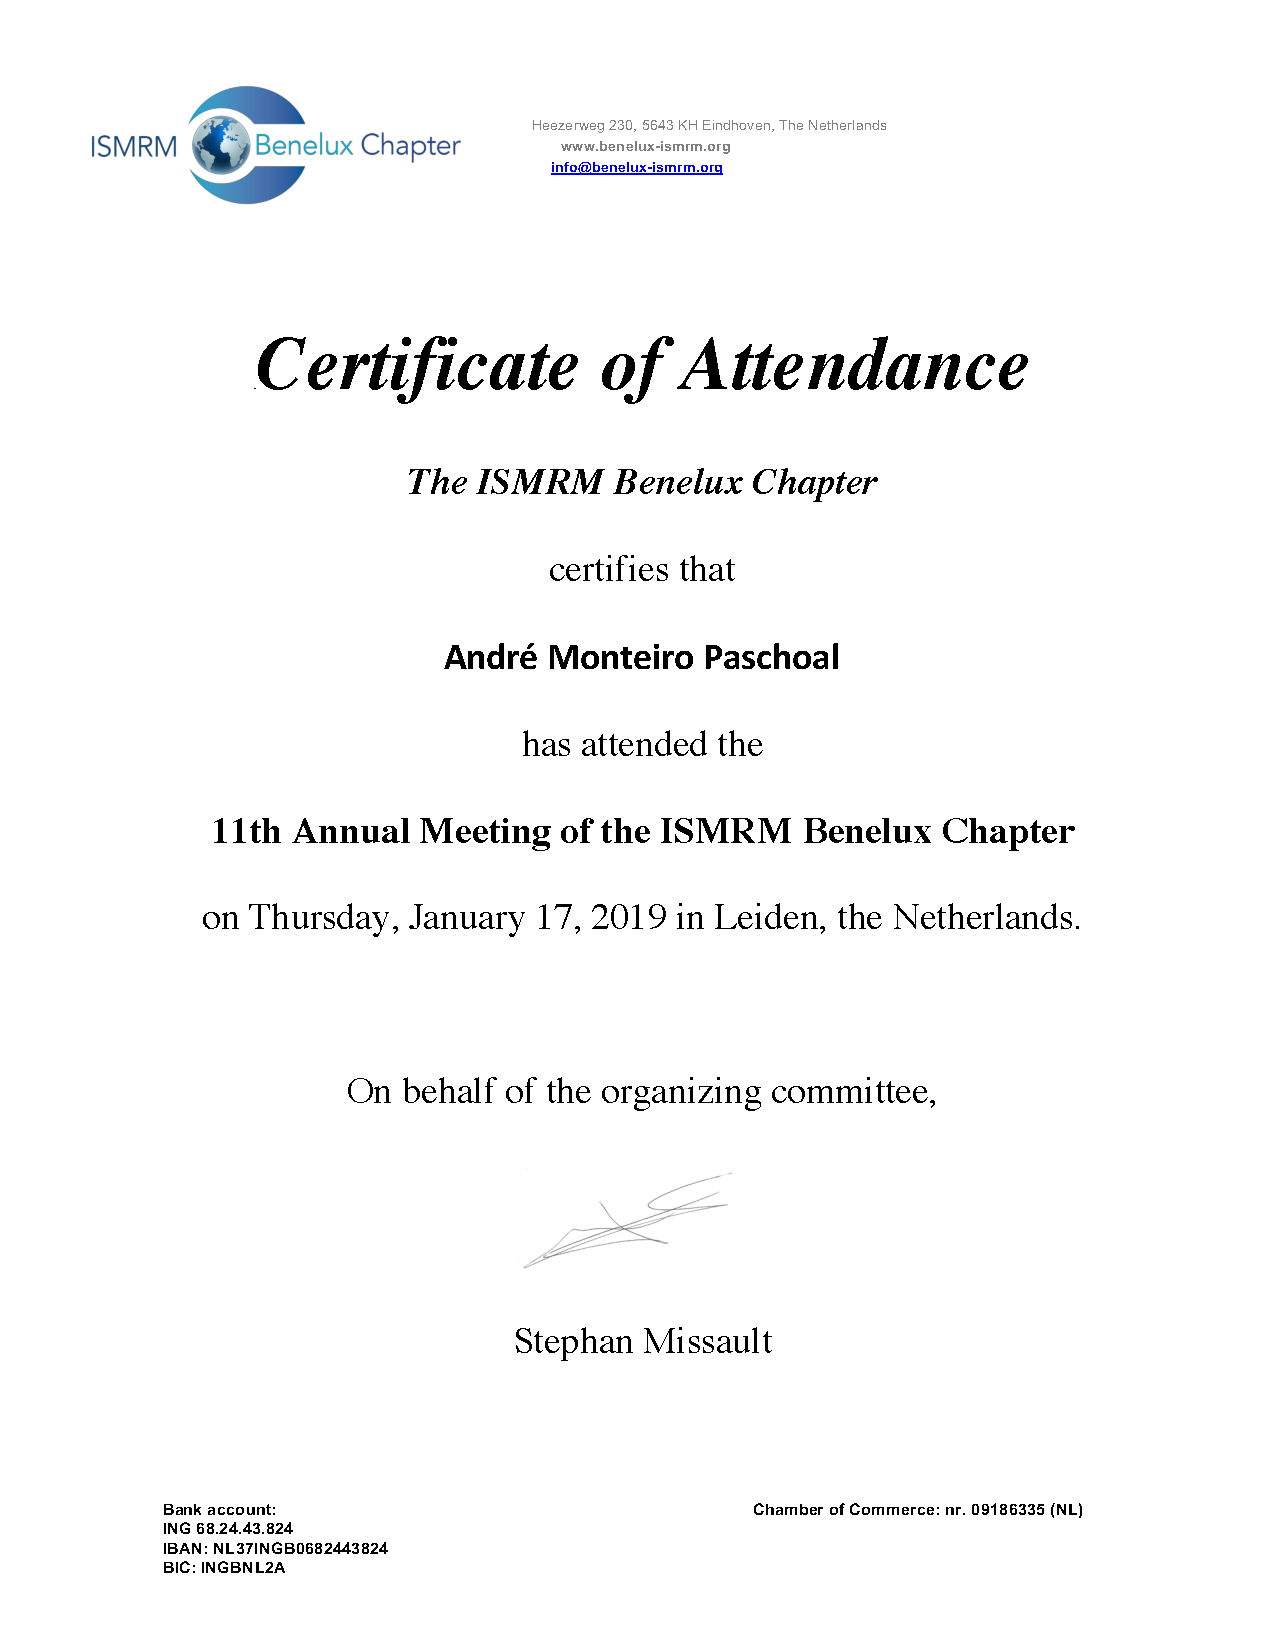
\includepdf[pages=-, scale=1,pagecommand=\thispagestyle{empty}]{\detokenize{Diplomas/certificate-ISMRMBenelux2019-Andre}}

\newpage
\subsection{Participa\c{c}\~{a}o em Eventos Cient\'{\i}ficos (com apresenta\c{c}\~{a}o de trabalho ou oferecimento de cursos, palestras ou debates}
\label{certificados:OHBM2019}
Esta subseção apresenta o comprovante da participação no Organization for Human Brain Mapping Annual Meeting com seus respectivos propósitos. \\
Obs: Ese congresso não emite certificado de apresentação de trabalhos, apenas de participação no evento.
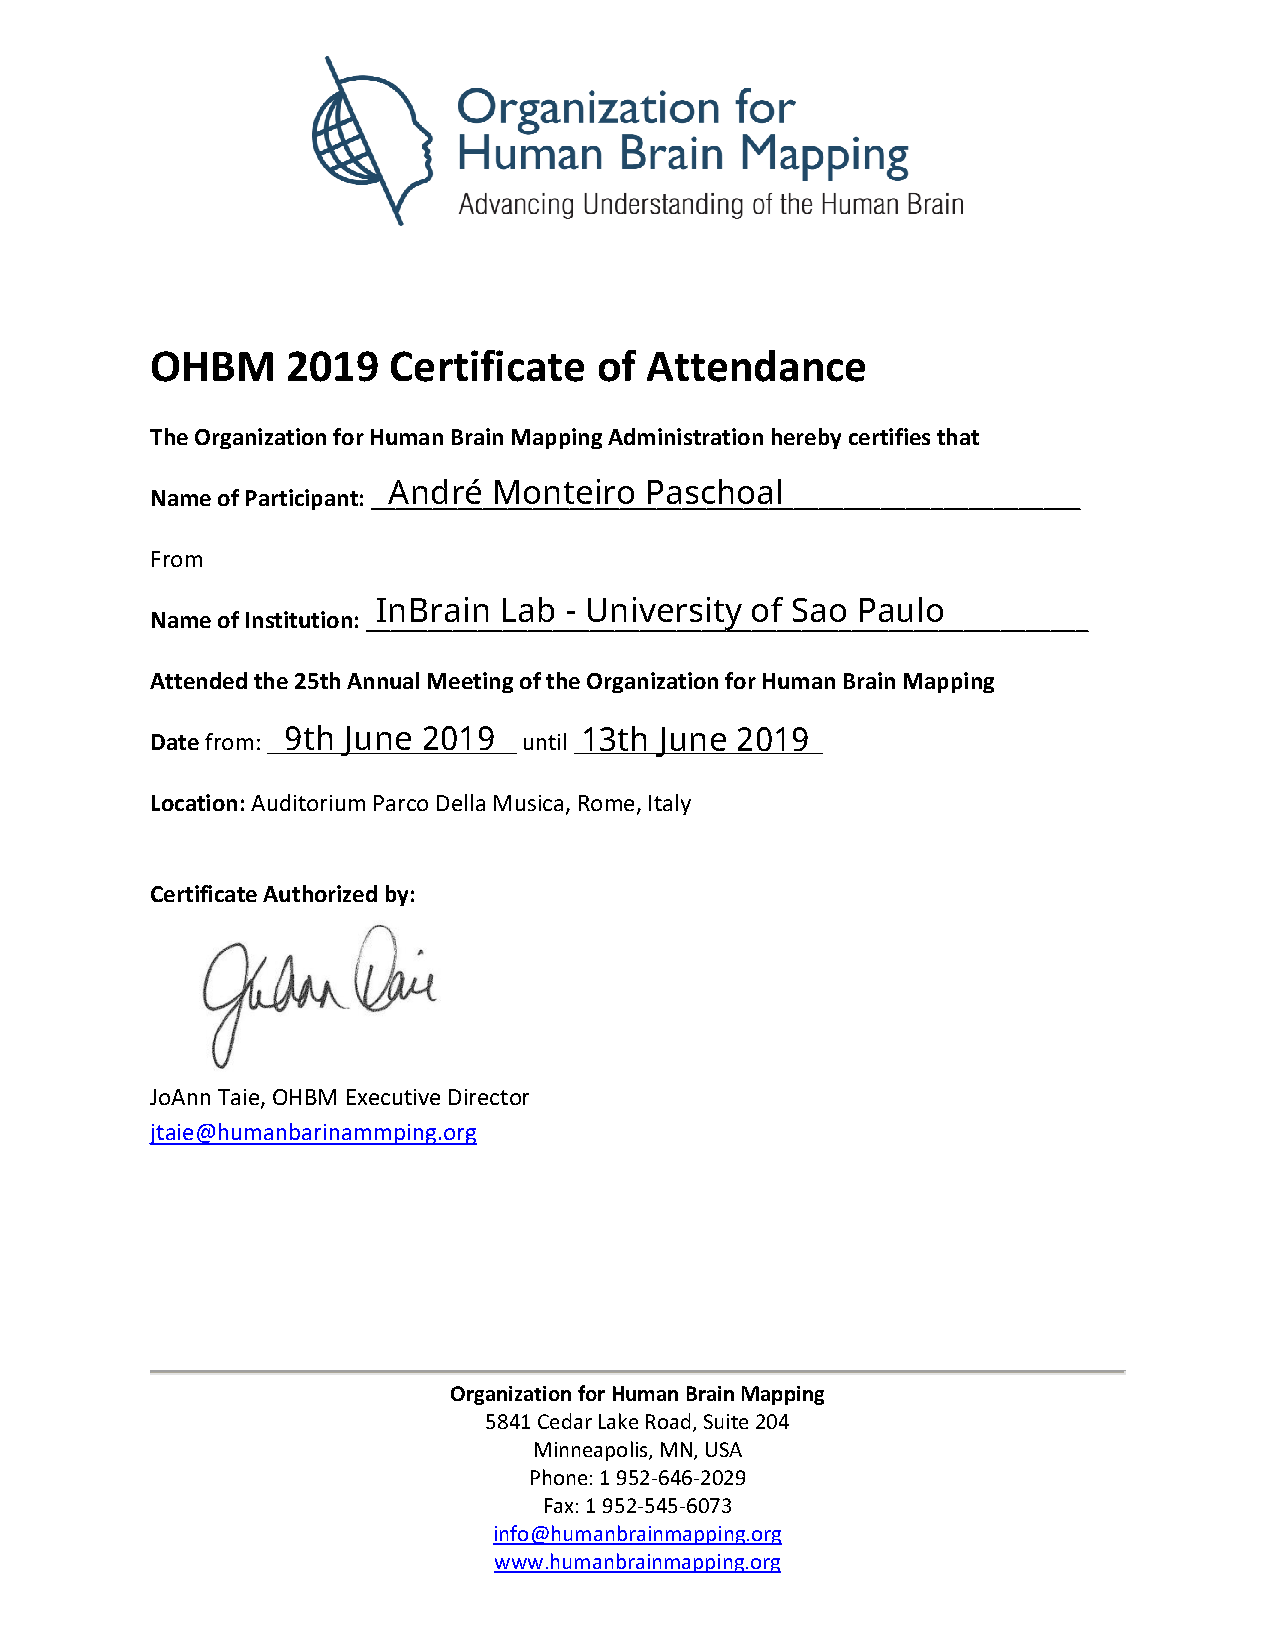
\includepdf[pages=-, scale=1,pagecommand=\thispagestyle{empty}]{\detokenize{Diplomas/Certificate of Attendance_OHBM-editado}}
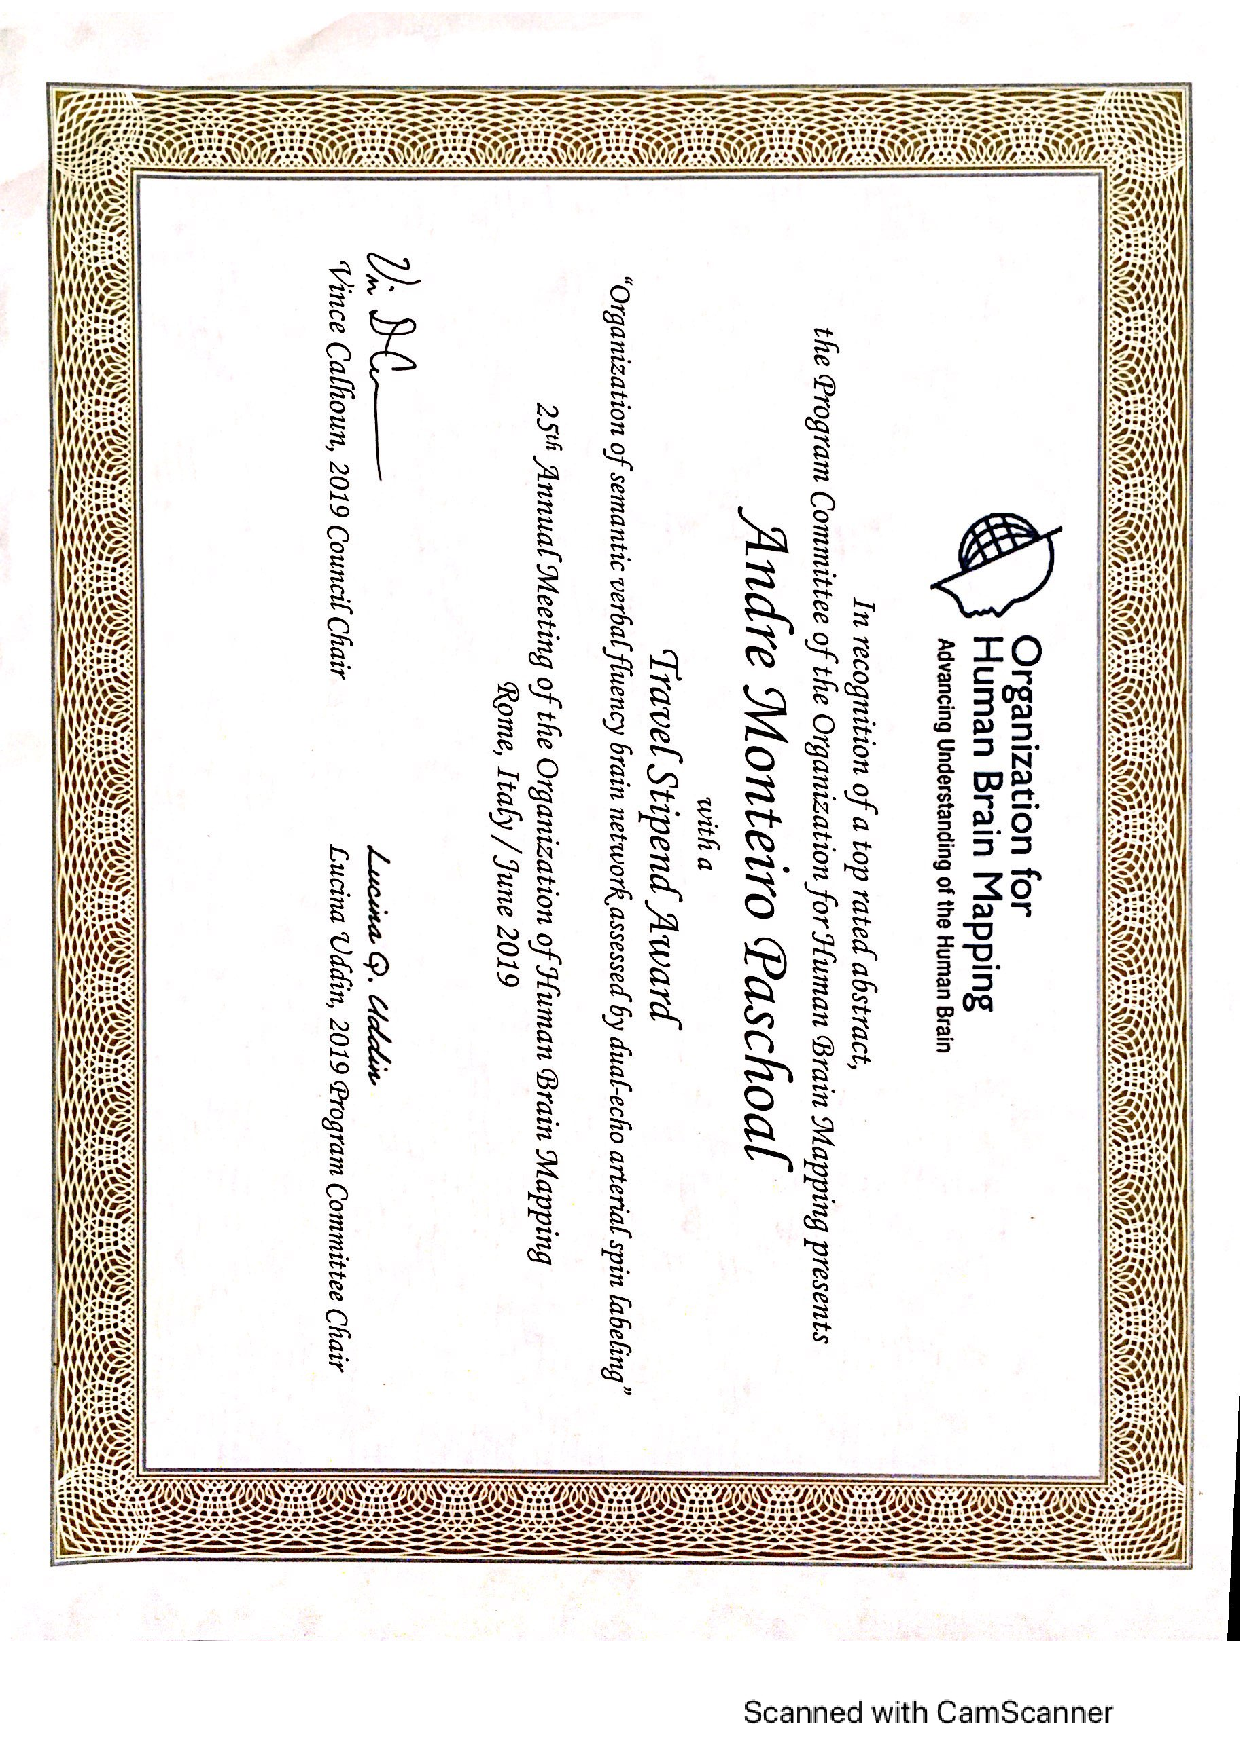
\includepdf[pages=-, scale=1,pagecommand=\thispagestyle{empty}]{\detokenize{Diplomas/OHBMtravelAward}}
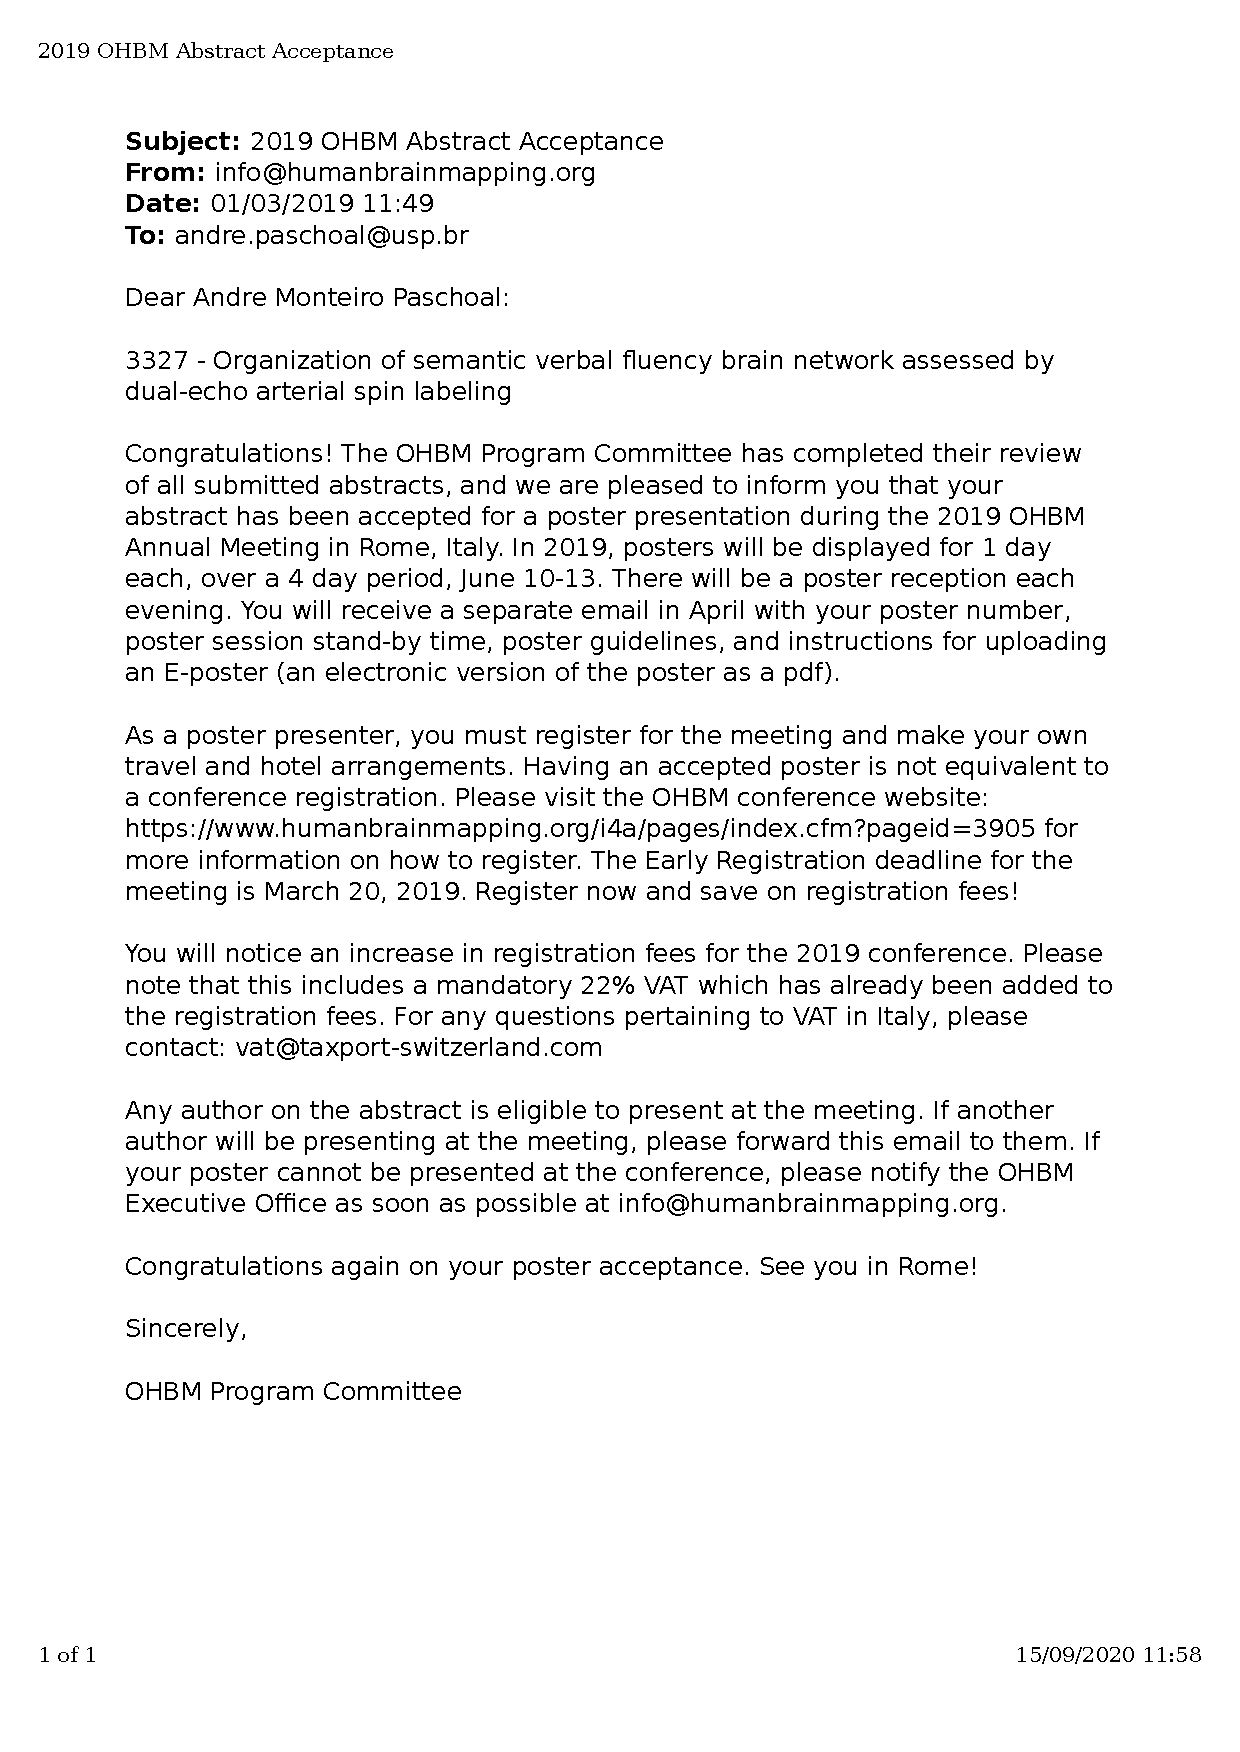
\includepdf[pages=-, scale=1,pagecommand=\thispagestyle{empty}]{\detokenize{Diplomas/AcceptanceOHBM2019}}

\newpage
\subsection{Participa\c{c}\~{a}o em Eventos Cient\'{\i}ficos (com apresenta\c{c}\~{a}o de trabalho ou oferecimento de cursos, palestras ou debates}
\label{certificados:SFM2019}
Esta subseção apresenta o comprovante da participação na XV Semana da Física Médica com seus respectivos propósitos.
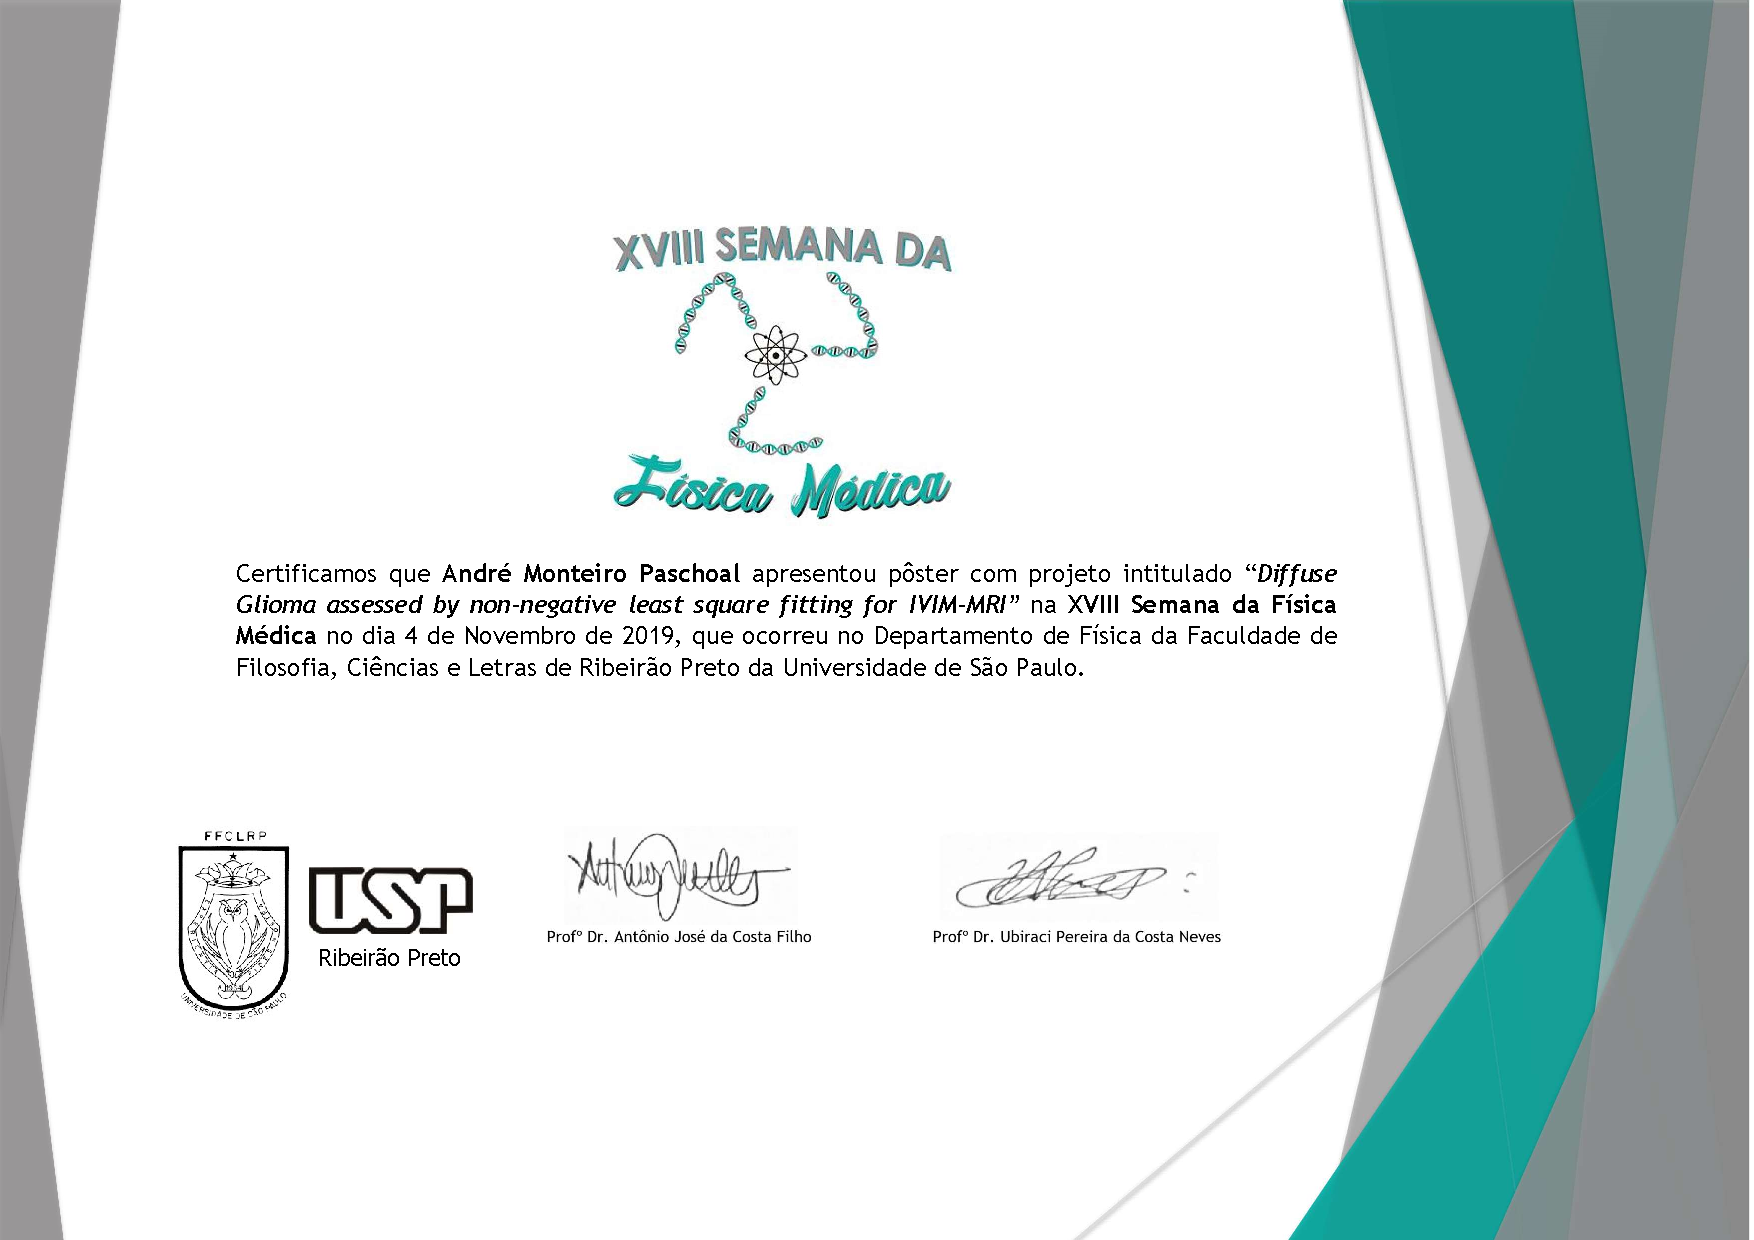
\includepdf[pages=-, scale=1,pagecommand=\thispagestyle{empty}]{\detokenize{Diplomas/SFM2019}}

\newpage
\subsection{Participa\c{c}\~{a}o em Eventos Cient\'{\i}ficos (com apresenta\c{c}\~{a}o de trabalho ou oferecimento de cursos, palestras ou debates}
\label{certificados:mrtrix3}
Esta subseção apresenta o comprovante da participação no 3rd MRTrix 3 Workshop com seus respectivos propósitos.
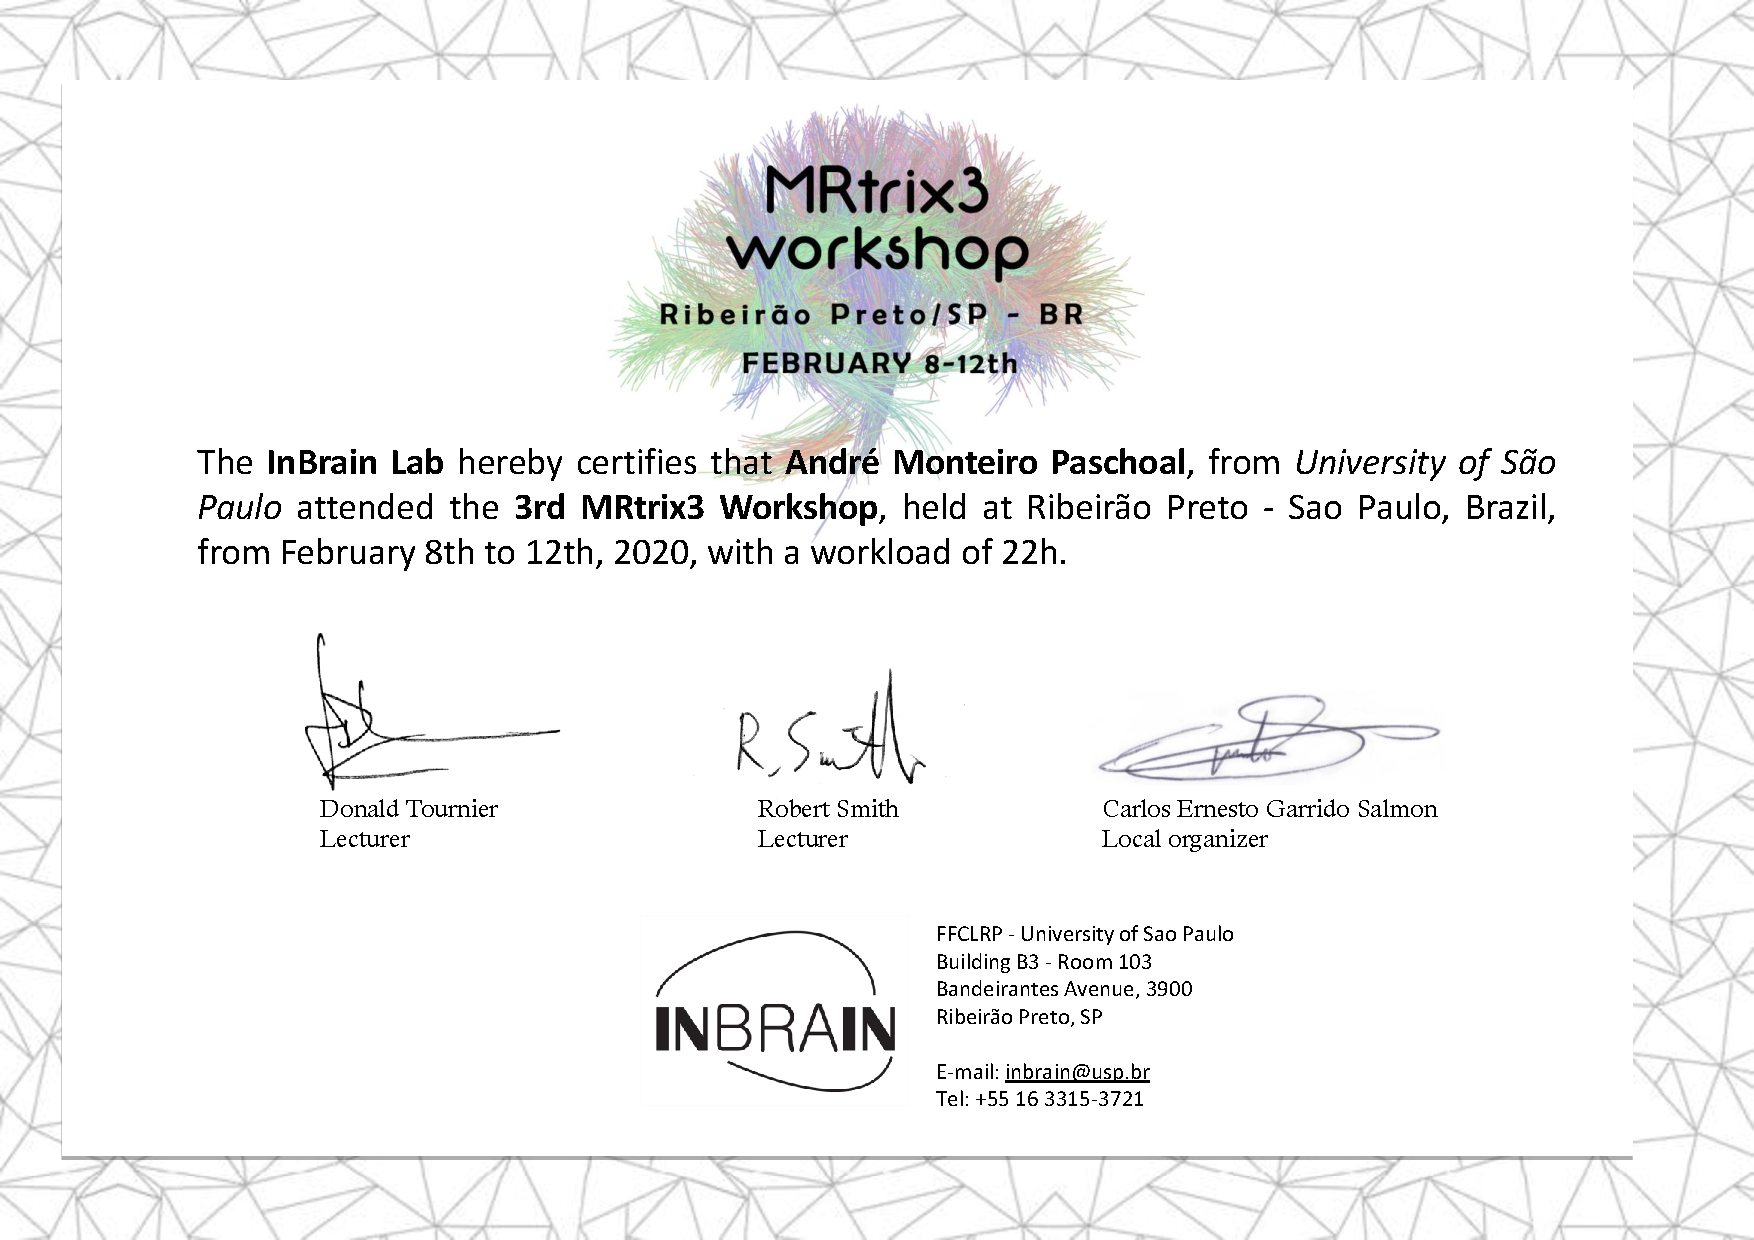
\includepdf[pages=-, scale=1,pagecommand=\thispagestyle{empty}]{\detokenize{Diplomas/mrtrix3workshop}}

\newpage
\subsection{Participa\c{c}\~{a}o em Eventos Cient\'{\i}ficos (com apresenta\c{c}\~{a}o de trabalho ou oferecimento de cursos, palestras ou debates}
\label{certificados:inbrain2020}
Esta subseção apresenta o comprovante da participação no InBrain Workshop 2020: Advanced Brain Imaging com seus respectivos propósitos.
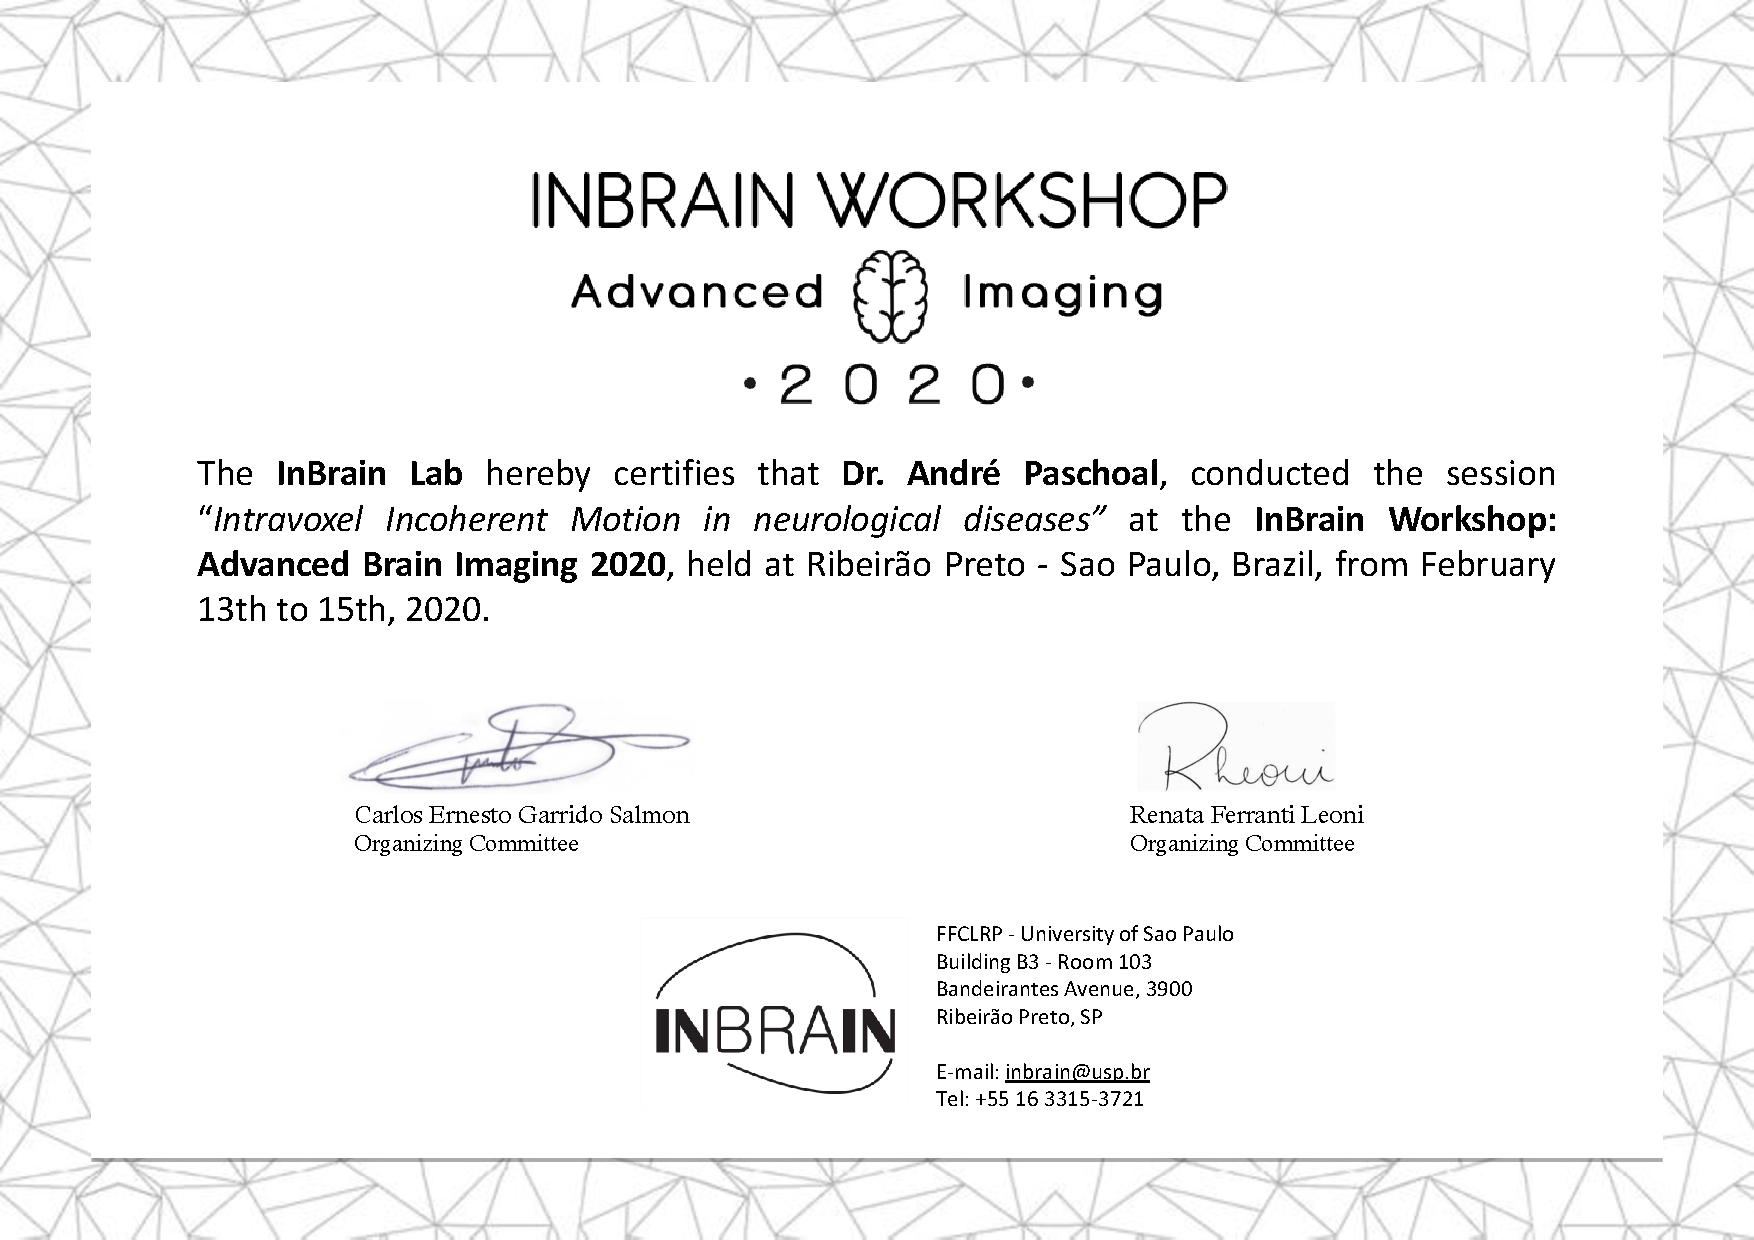
\includepdf[pages=-, scale=1,pagecommand=\thispagestyle{empty}]{\detokenize{Diplomas/InBrainWorkshop_palestrante}}

\newpage
\subsection{Participa\c{c}\~{a}o em Eventos Cient\'{\i}ficos (com apresenta\c{c}\~{a}o de trabalho ou oferecimento de cursos, palestras ou debates}
\label{certificados:ISMRM2020}
Esta subseção apresenta o comprovante da participação no 
ISMRM 28th Annual Meeting \& Exhibition com seus respectivos propósitos. \\
%Obs: Ese congresso não emite certificado de apresentação de trabalhos, apenas de participação no evento.
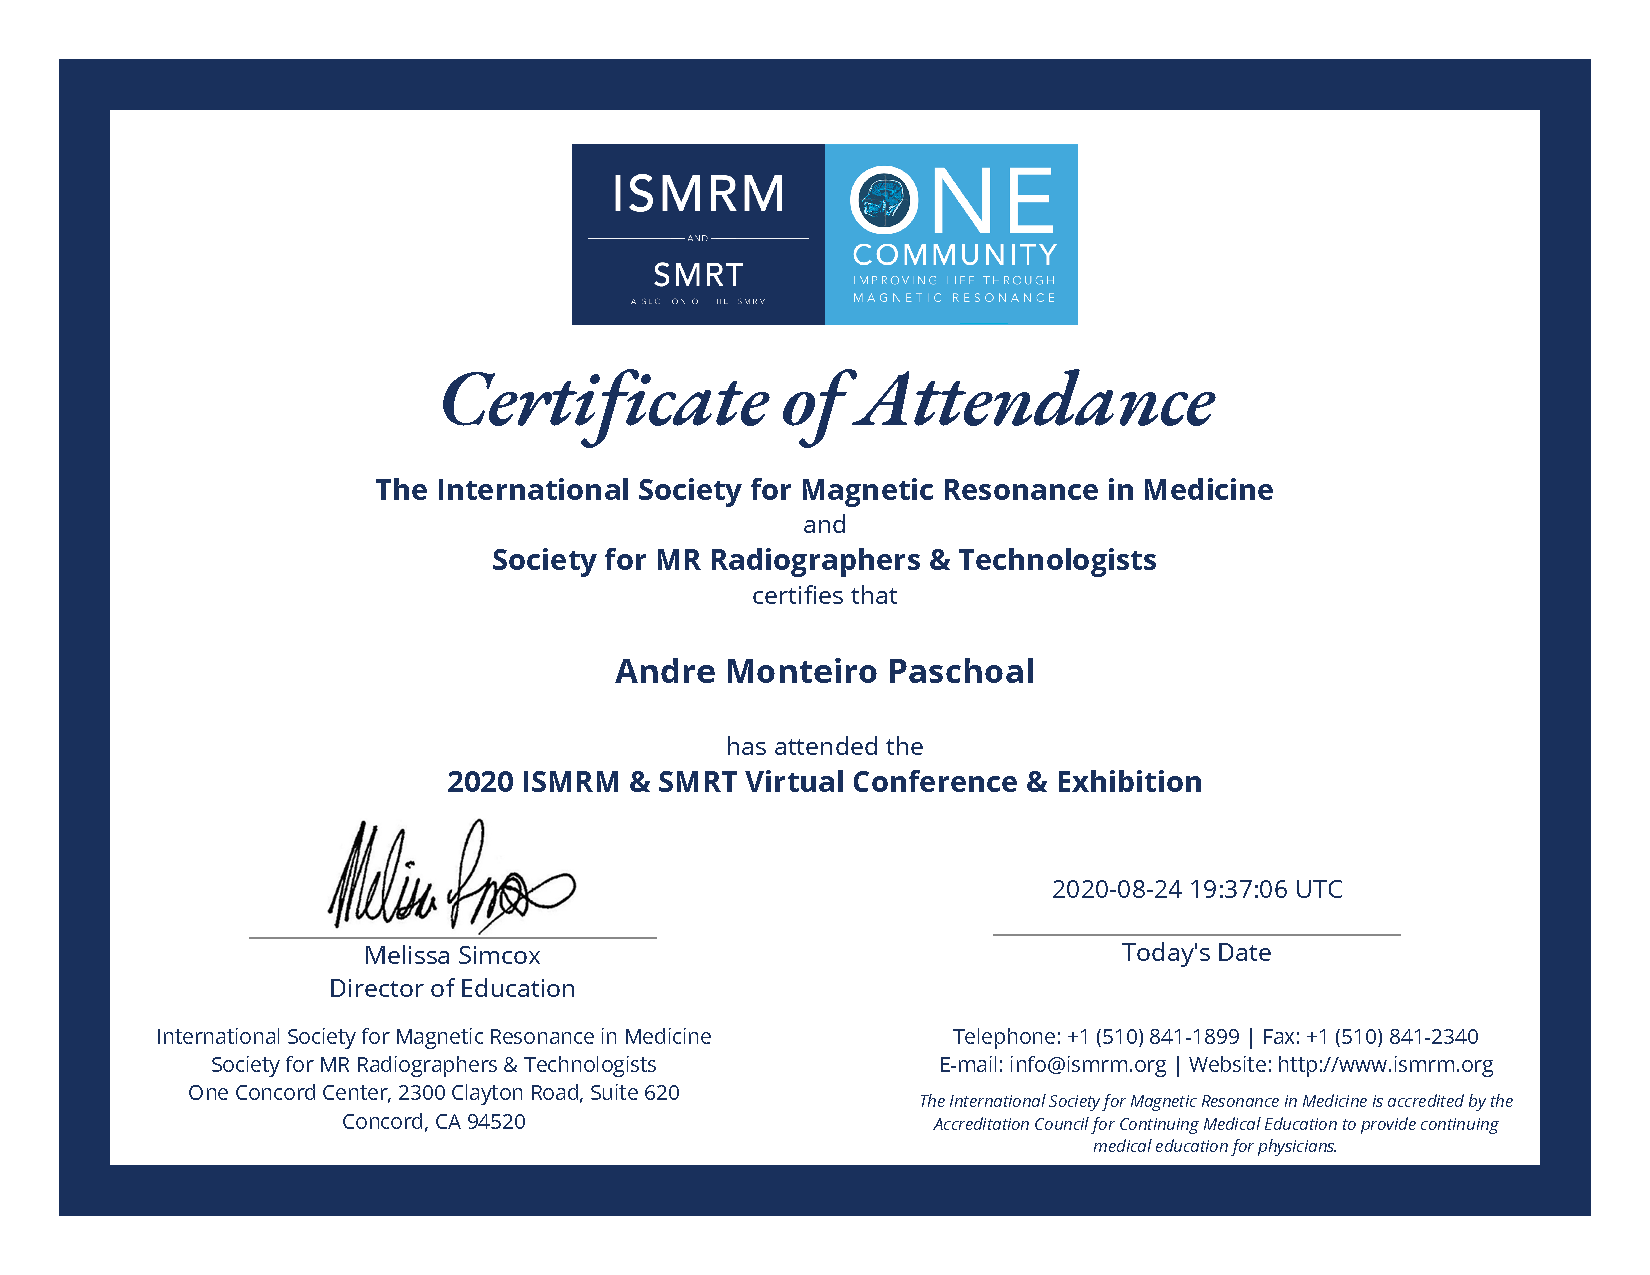
\includepdf[pages=-, scale=1,pagecommand=\thispagestyle{empty}]{\detokenize{Diplomas/ISMRM2020}}
%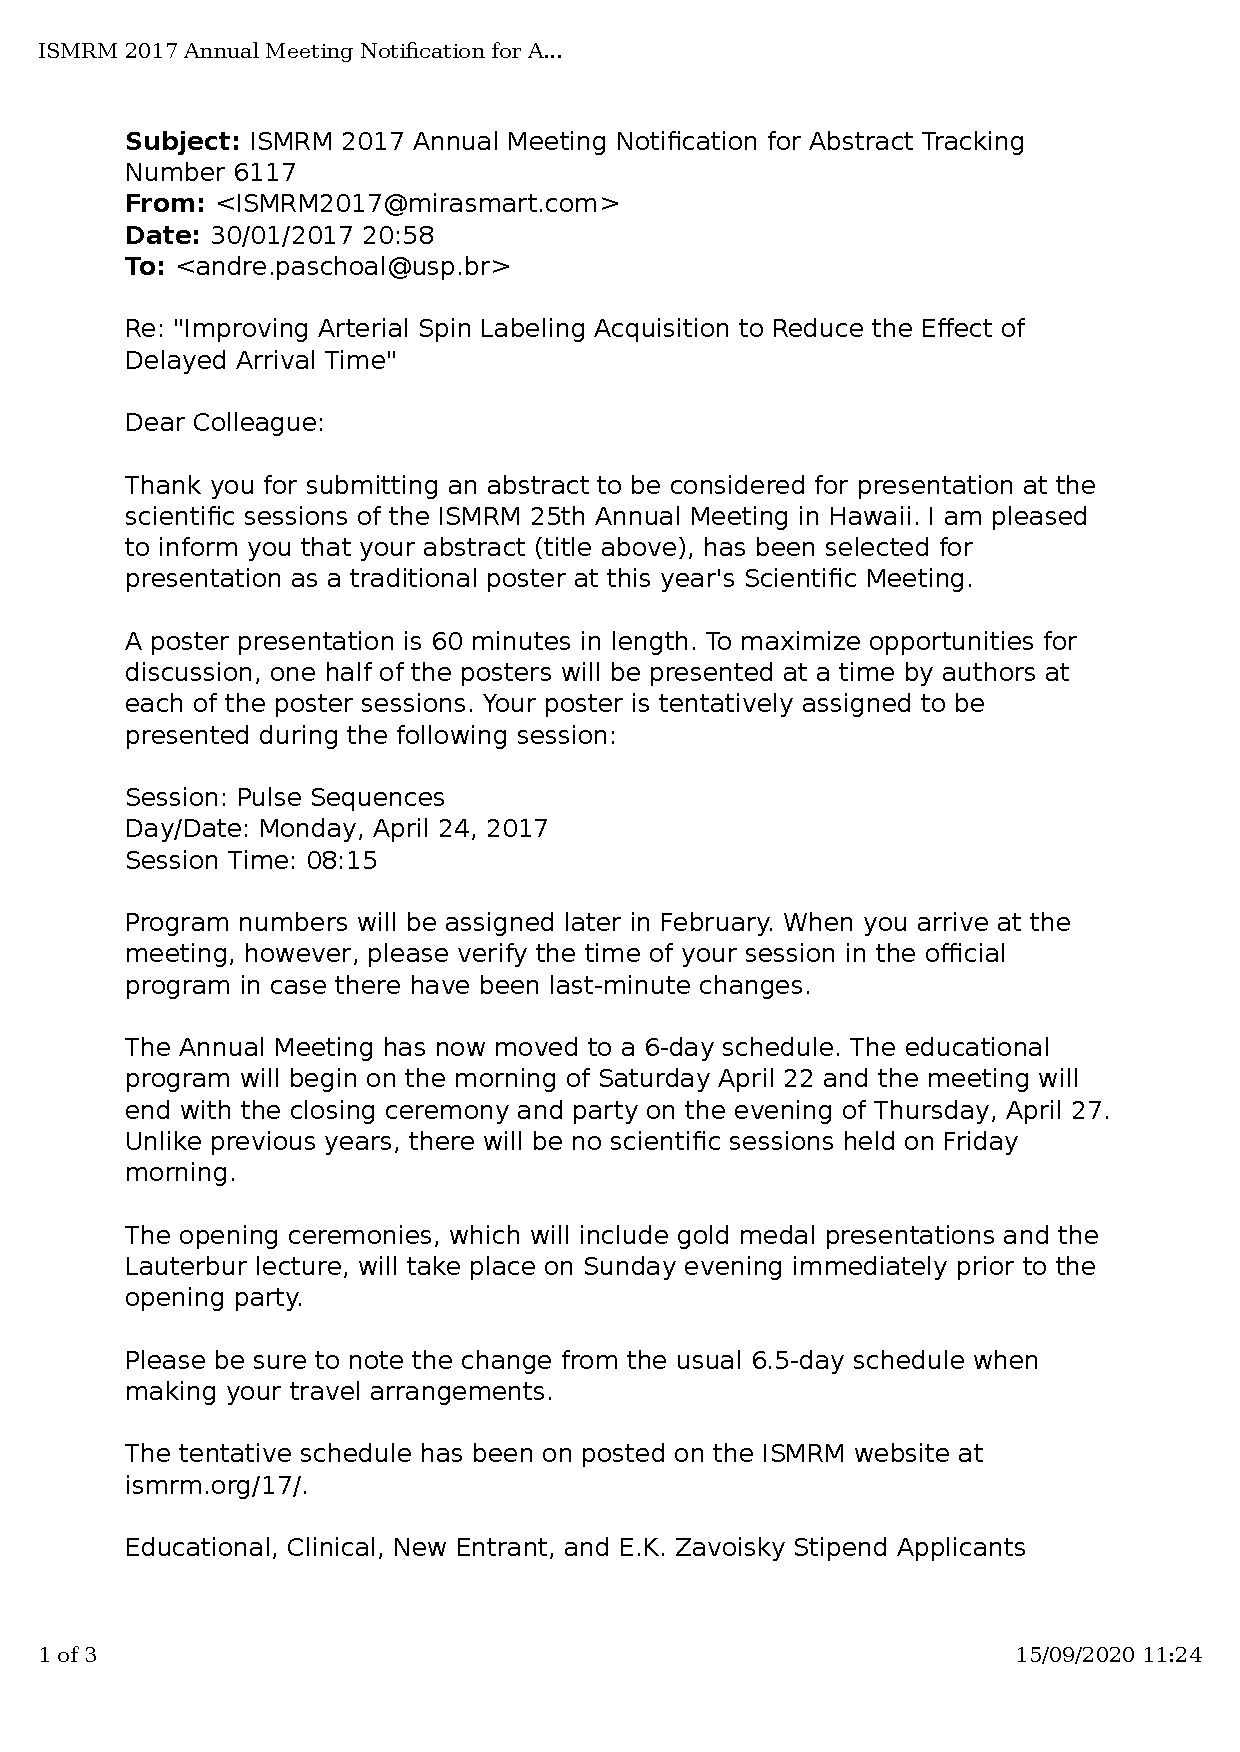
\includepdf[pages=-, scale=1,pagecommand=\thispagestyle{empty}]{\detokenize{Diplomas/AcceptanceISMRM2017}}

\newpage
\subsection{Participa\c{c}\~{a}o em Eventos Cient\'{\i}ficos (com apresenta\c{c}\~{a}o de trabalho ou oferecimento de cursos, palestras ou debates}
\label{certificados:ESMRMB2020}
Esta subseção apresenta o comprovante da participação no 
ESMRMB 37th Annual Meeting \& Exhibition com seus respectivos propósitos. \\
Obs: Ese congresso não emite certificado de apresentação de trabalhos, apenas de participação no evento.
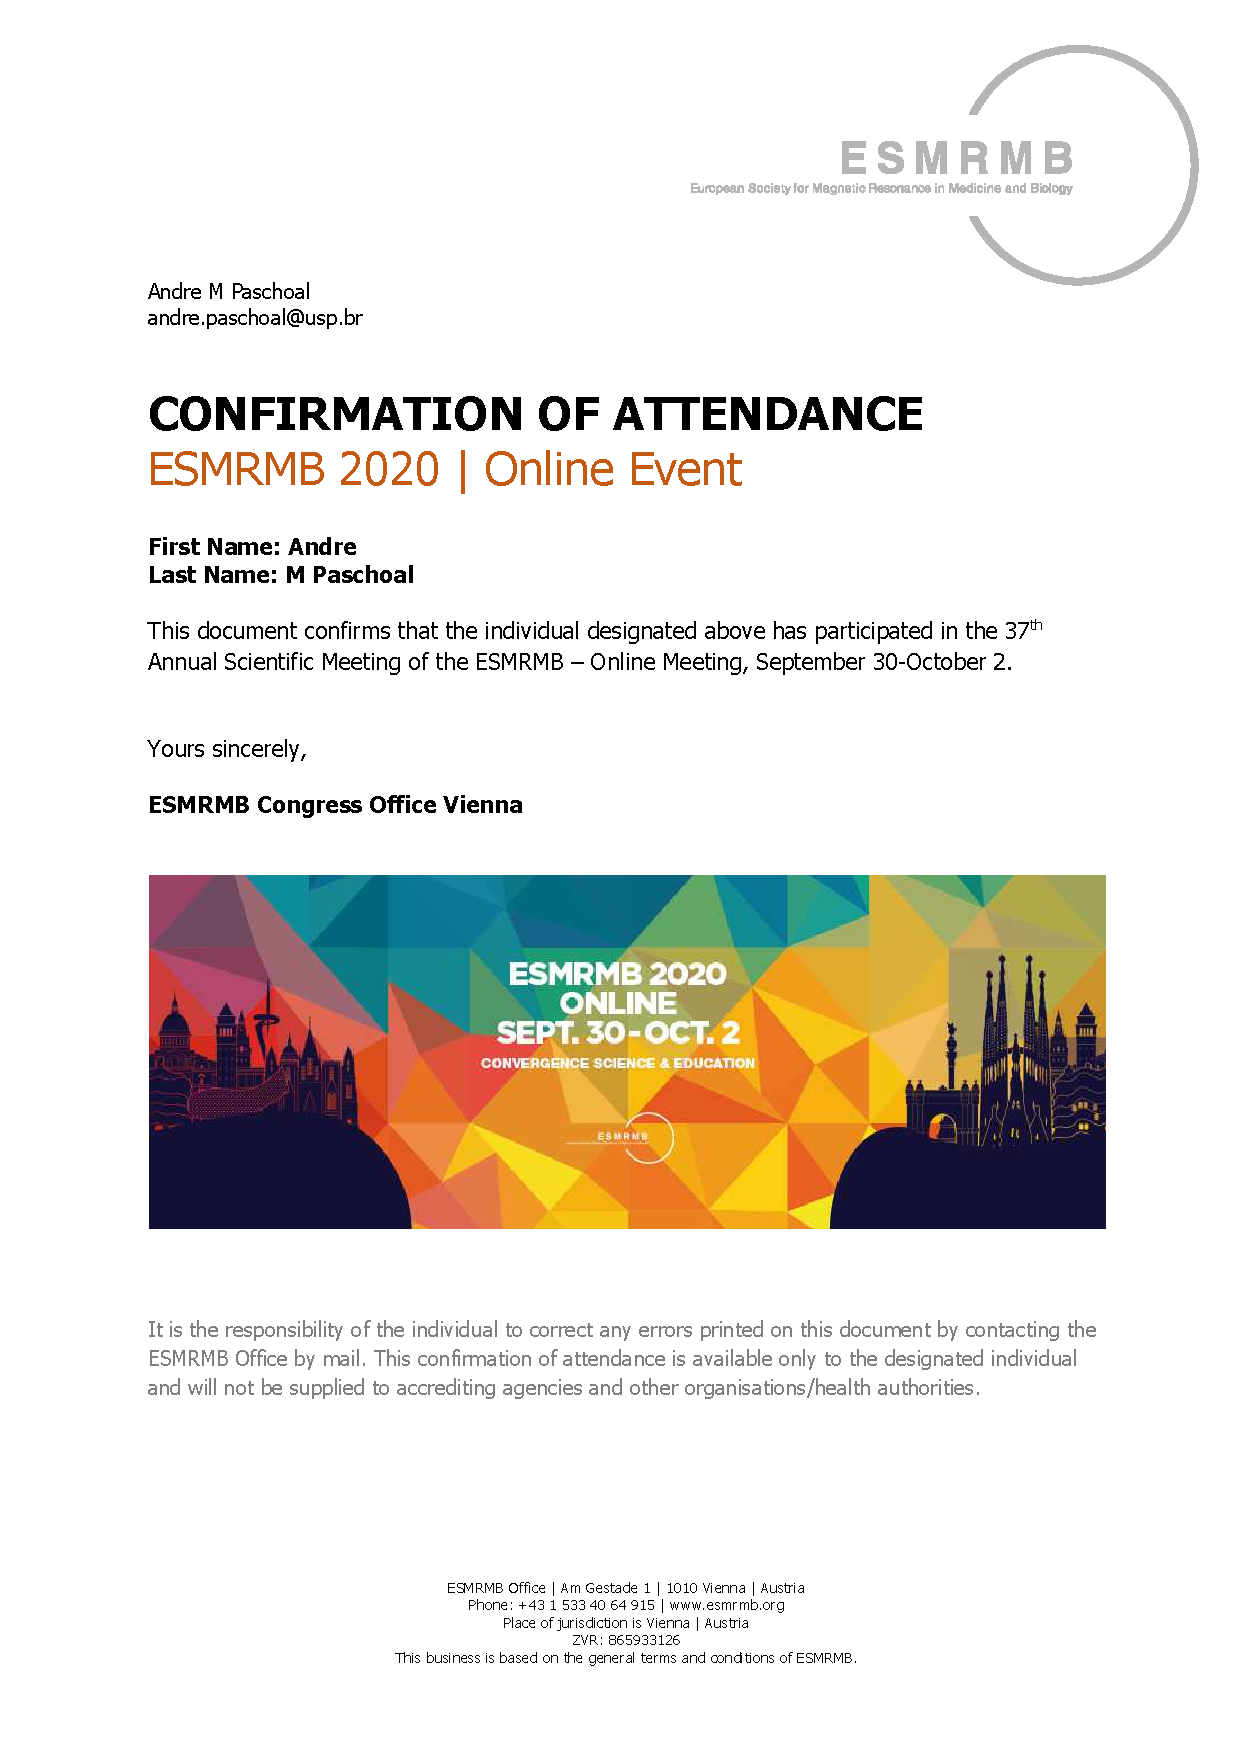
\includepdf[pages=-, scale=1,pagecommand=\thispagestyle{empty}]{\detokenize{Diplomas/ESMRMB2020}}
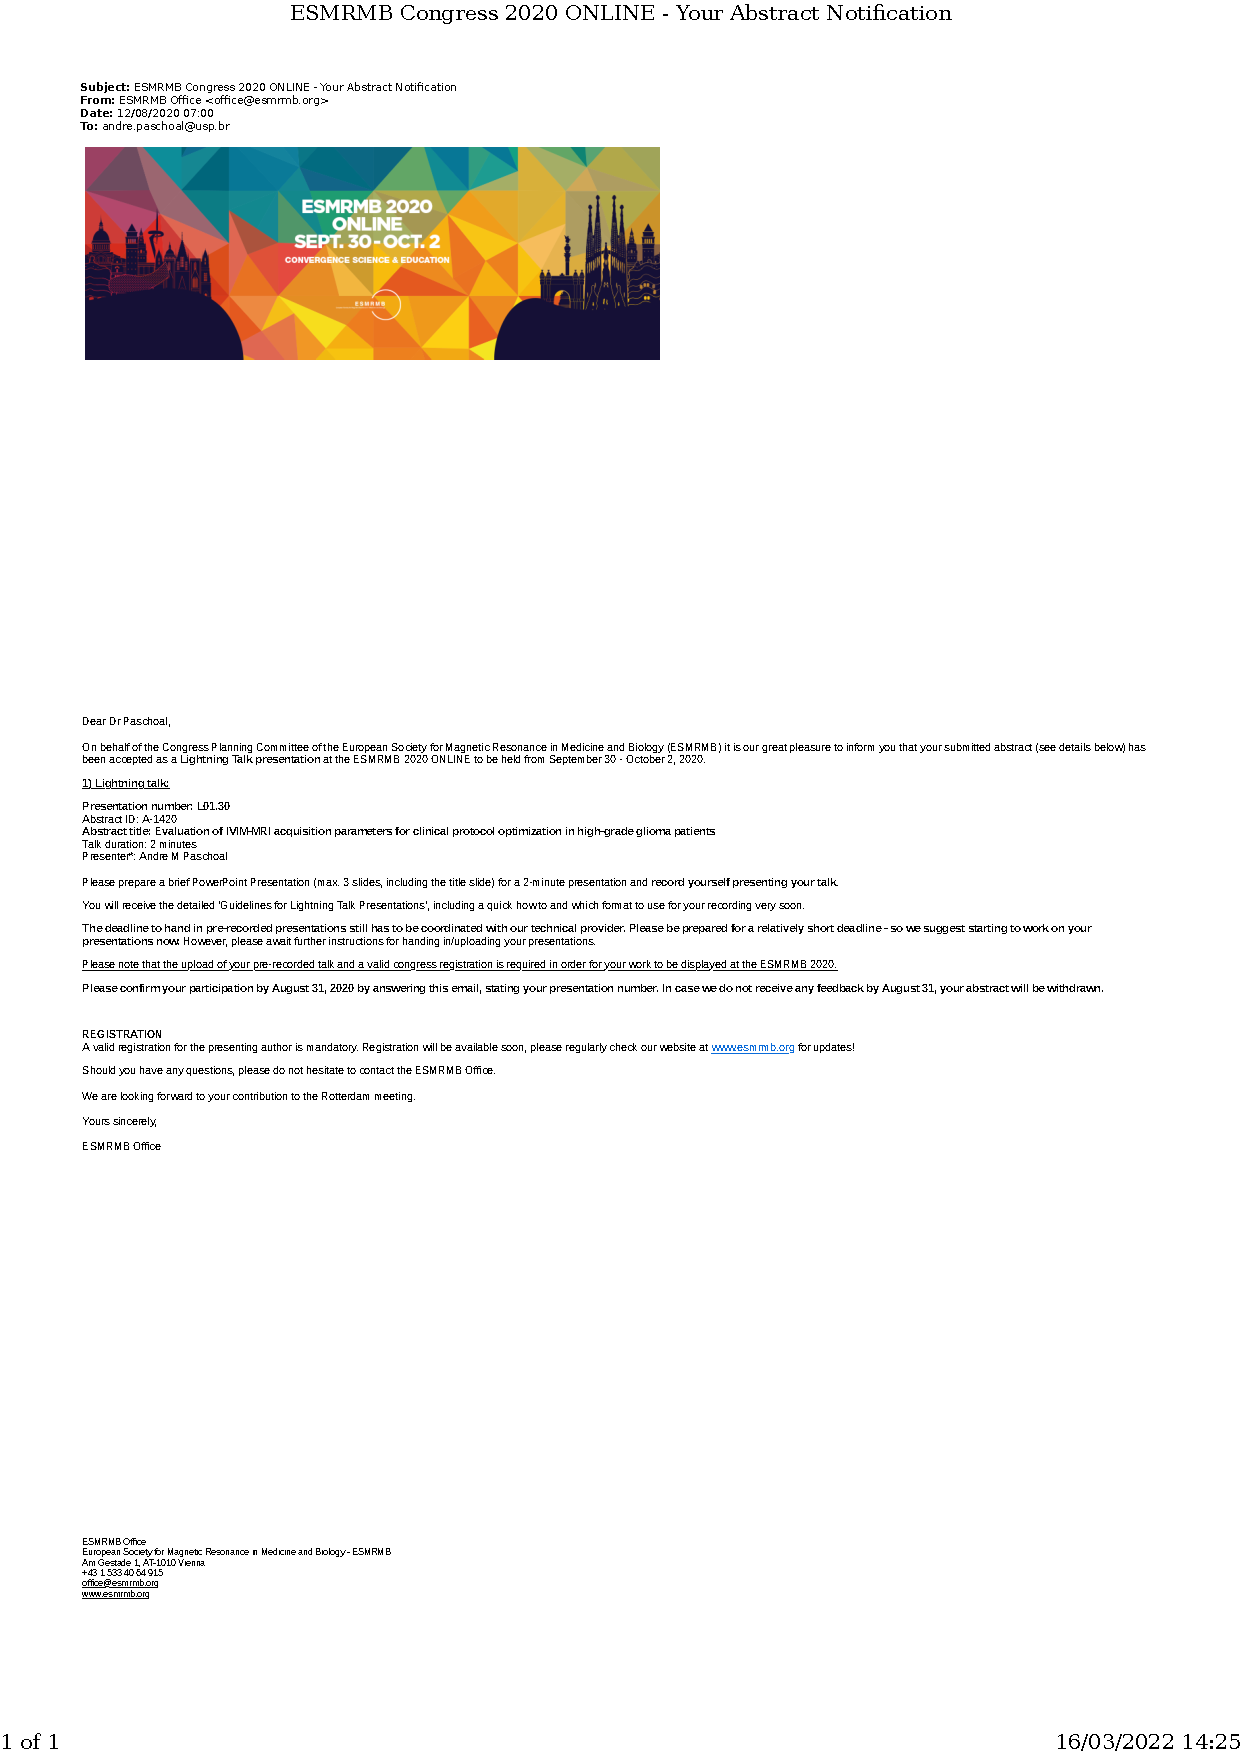
\includepdf[pages=-, scale=1,pagecommand=\thispagestyle{empty}]{\detokenize{Diplomas/AcceptanceESMRMB2020}}

\newpage
\subsection{Participa\c{c}\~{a}o em Eventos Cient\'{\i}ficos (com apresenta\c{c}\~{a}o de trabalho ou oferecimento de cursos, palestras ou debates}
\label{certificados:ISMRM2021}
Esta subseção apresenta o comprovante da participação no 
ISMRM 29th Annual Meeting \& Exhibition com seus respectivos propósitos. \\
Obs: Ese congresso não emite certificado de apresentação de trabalhos, apenas de participação no evento.
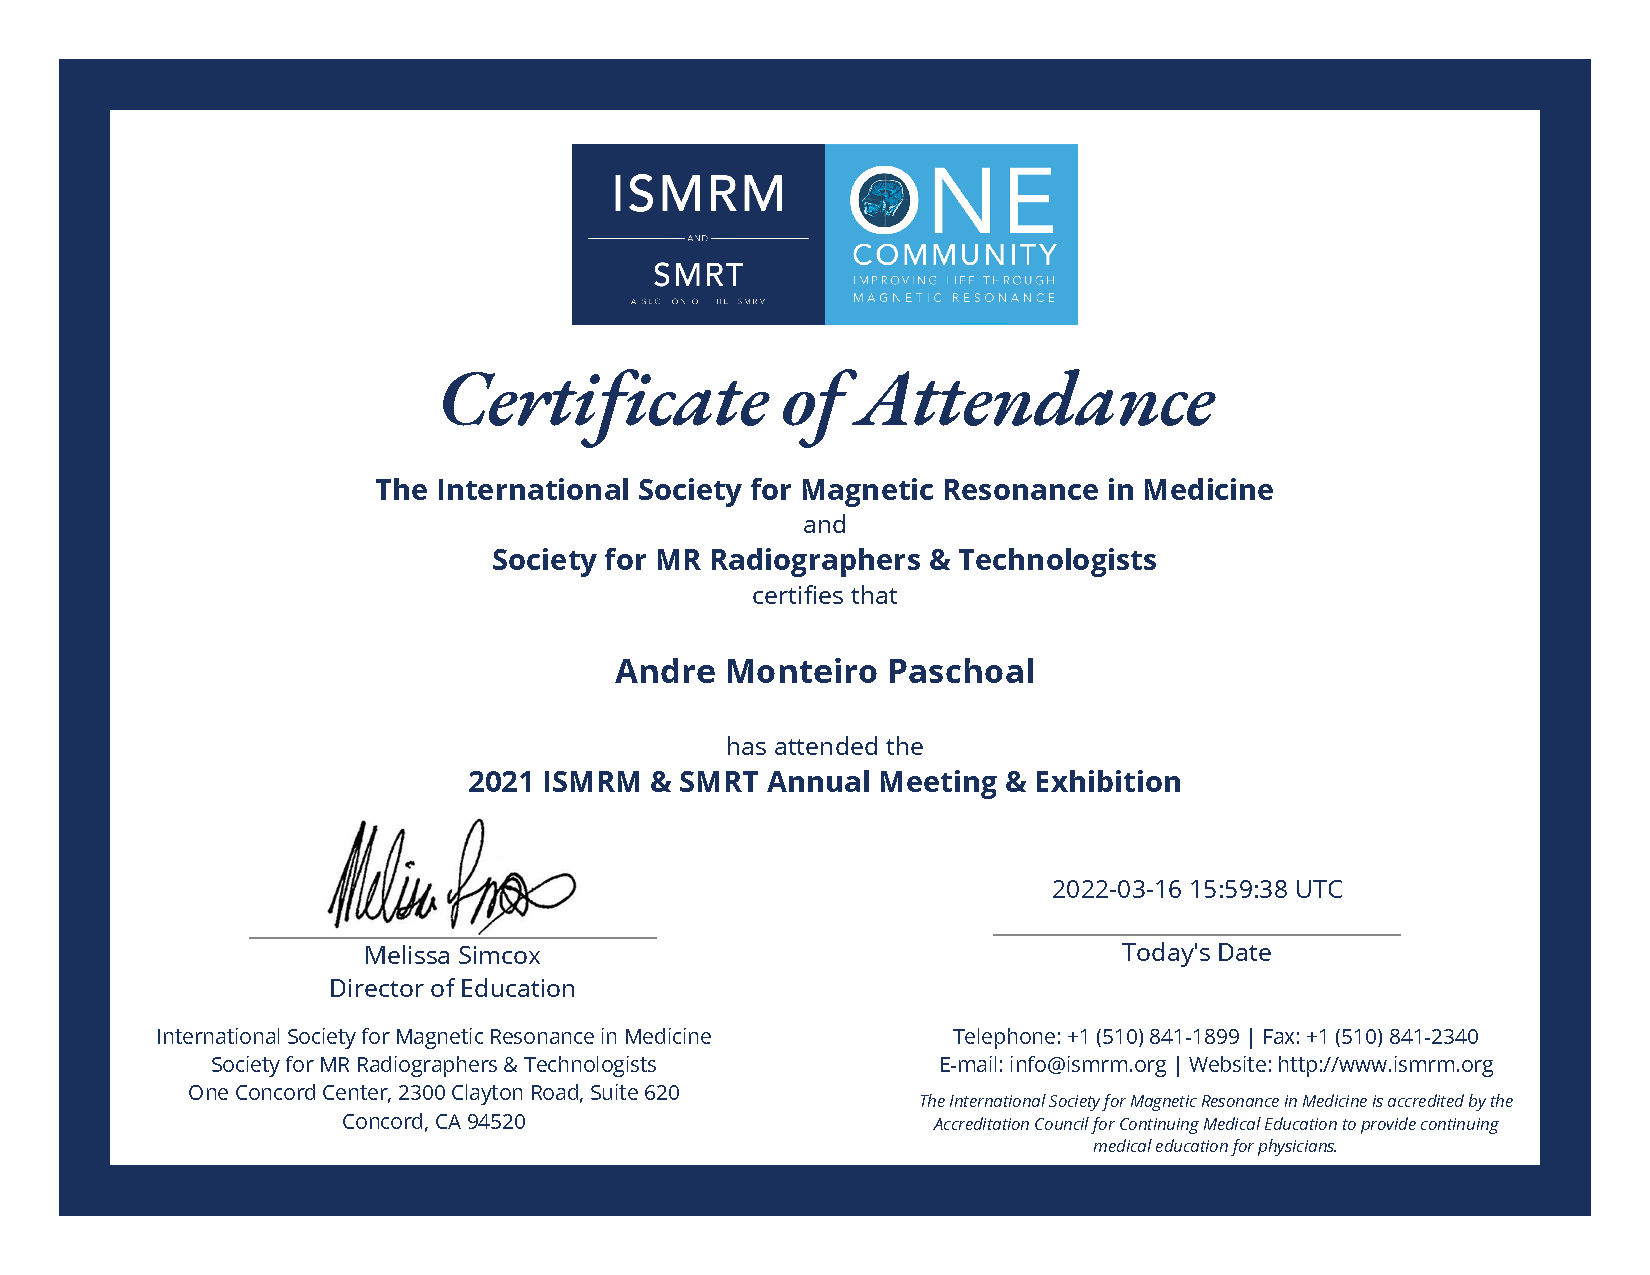
\includepdf[pages=-, scale=1,pagecommand=\thispagestyle{empty}]{\detokenize{Diplomas/ISMRM2021}}
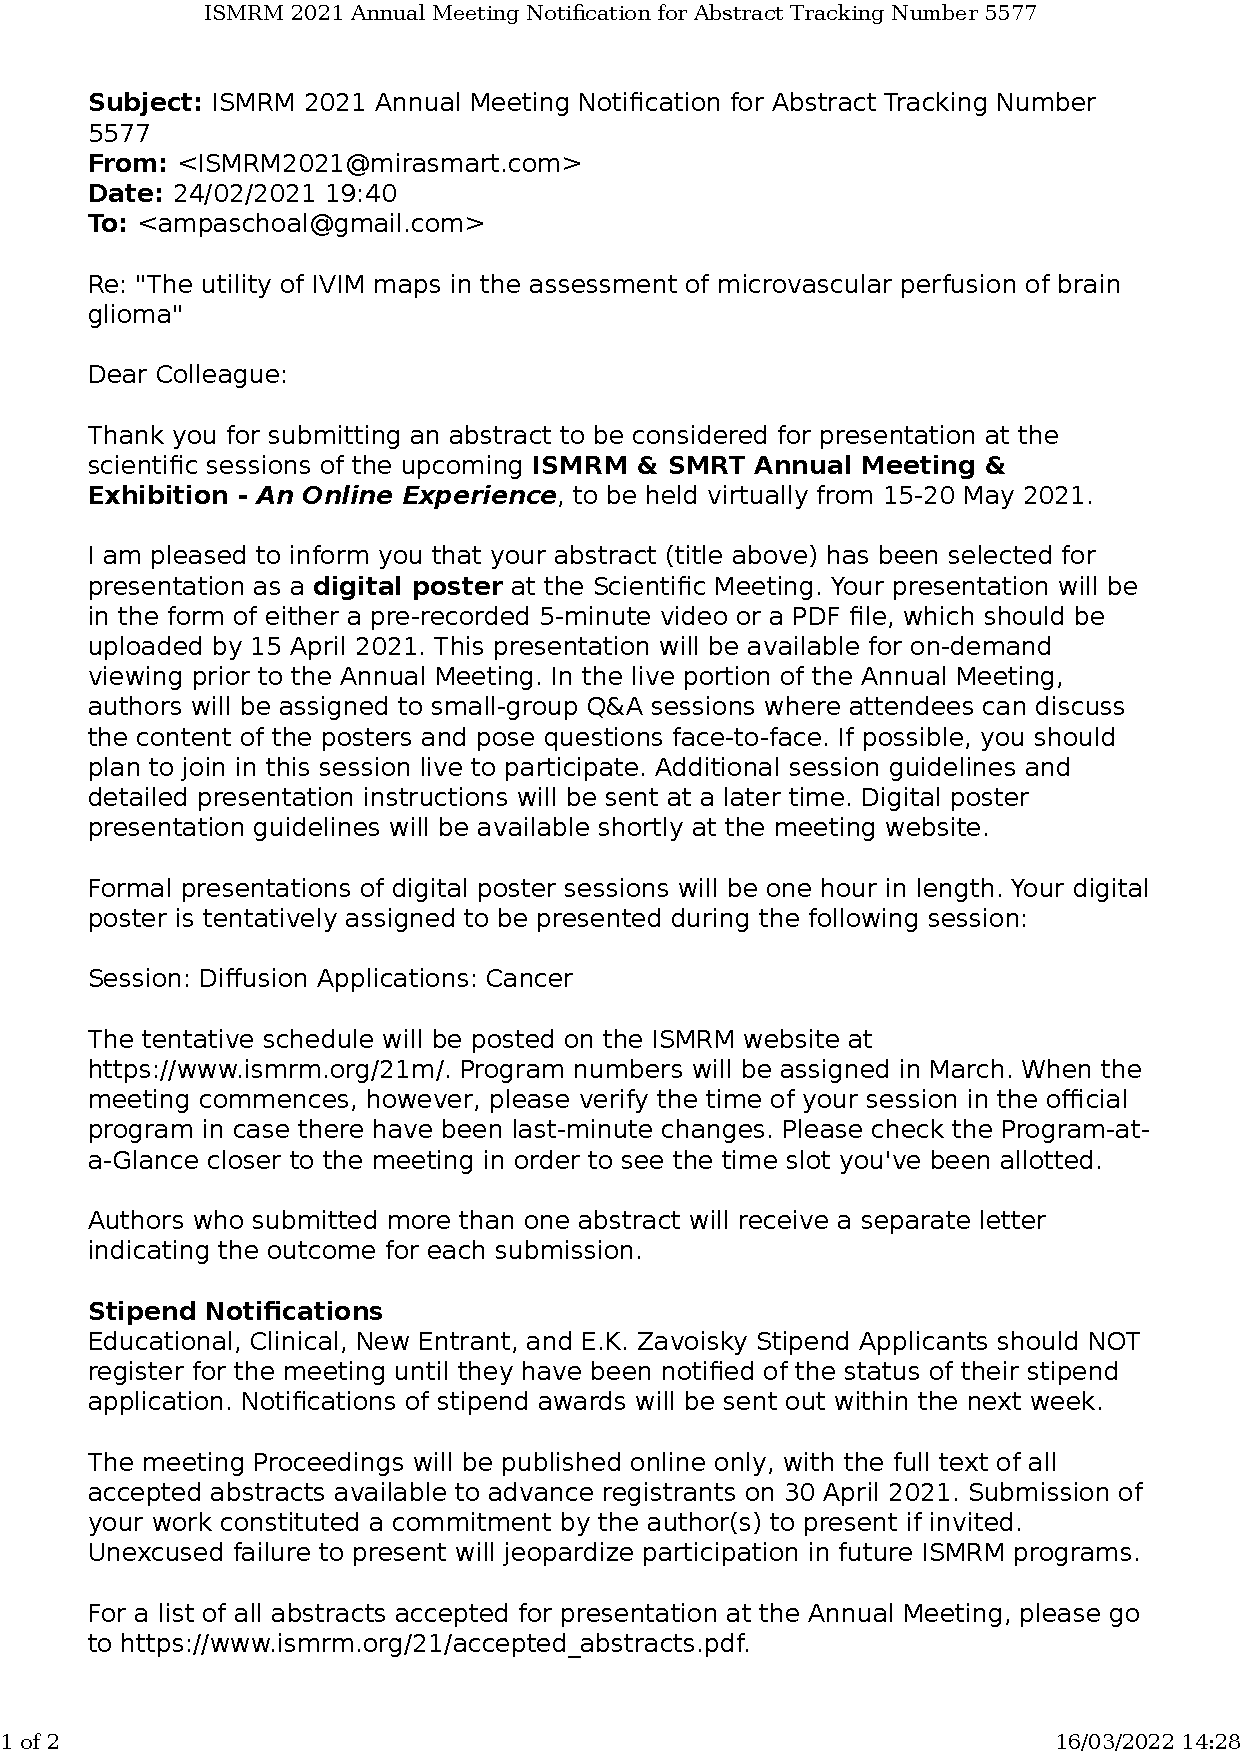
\includepdf[pages=-, scale=1,pagecommand=\thispagestyle{empty}]{\detokenize{Diplomas/AcceptanceISMRM2021_1}}
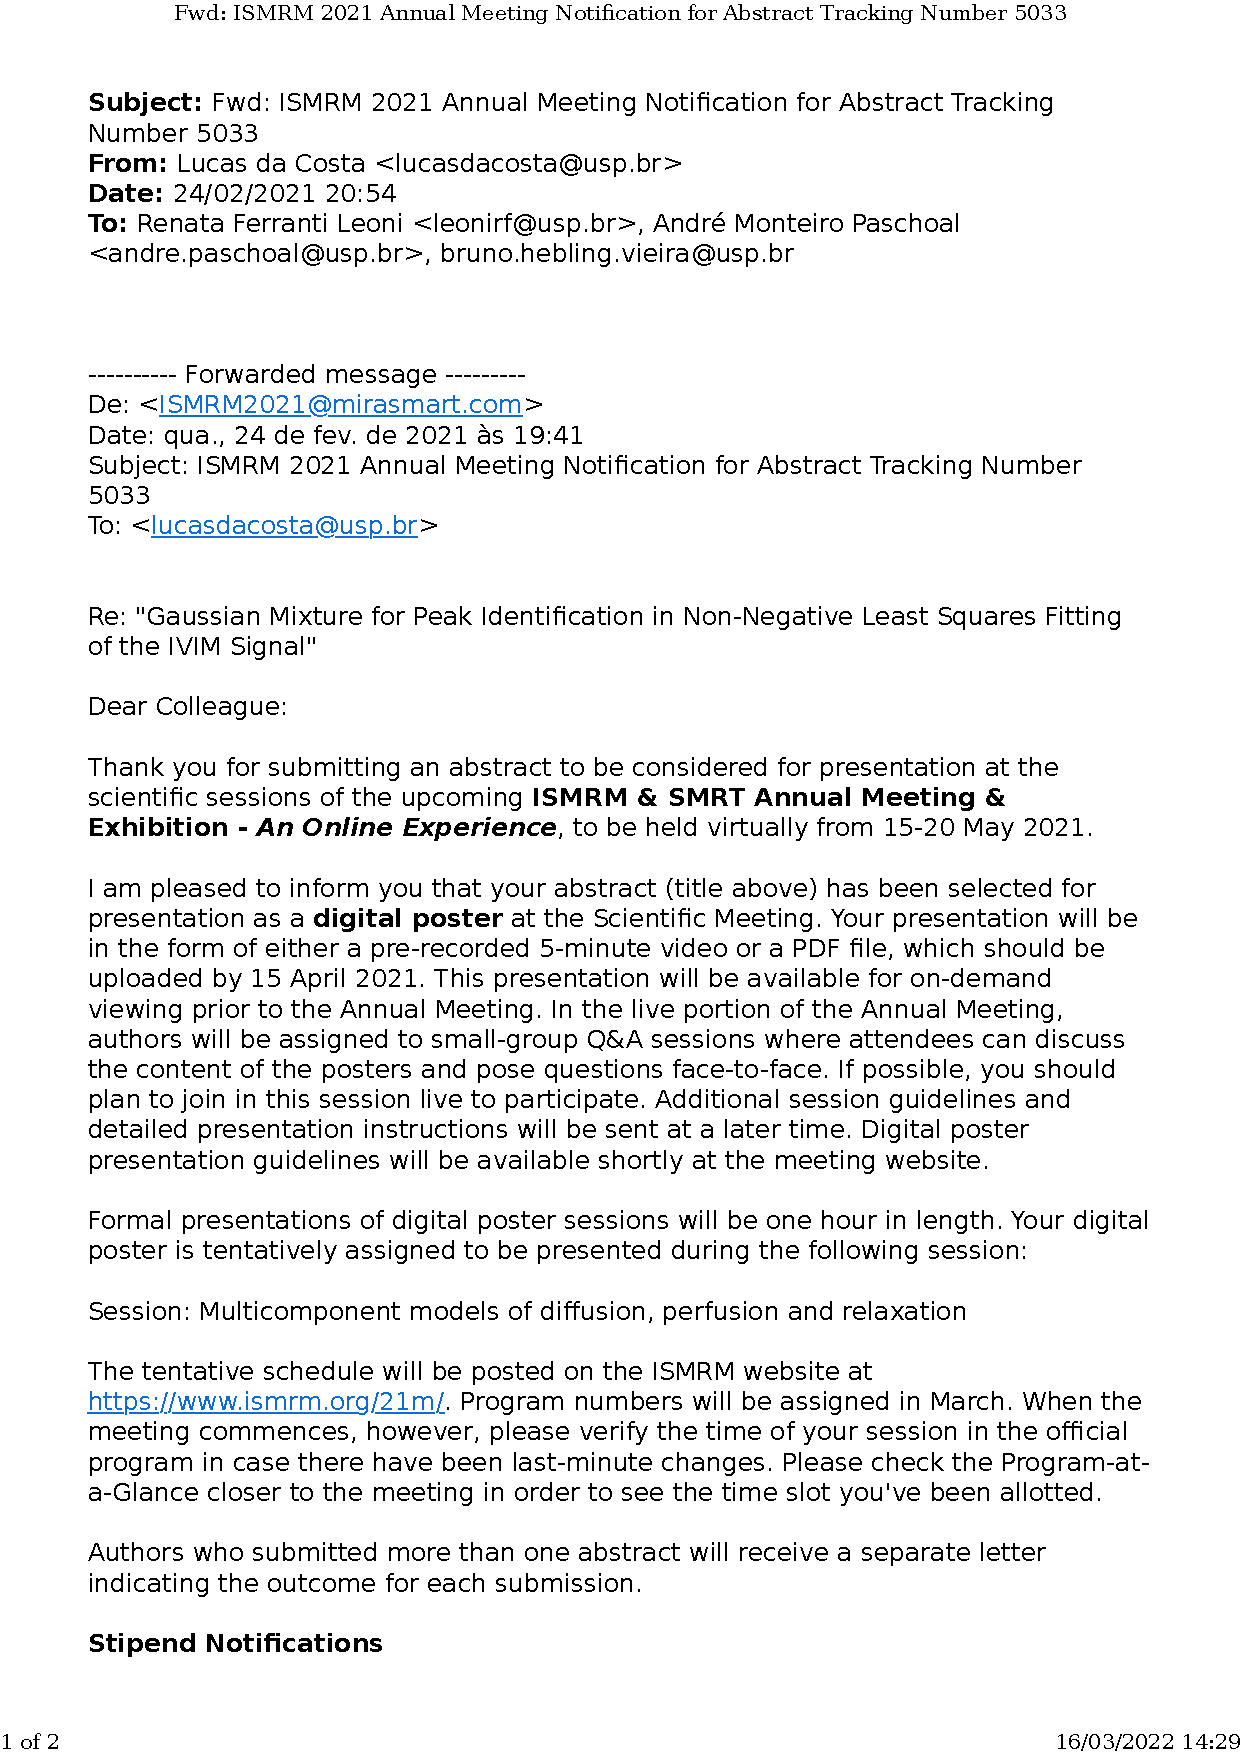
\includepdf[pages=-, scale=1,pagecommand=\thispagestyle{empty}]{\detokenize{Diplomas/AcceptanceISMRM2021_2}}

\newpage
\subsection{Participa\c{c}\~{a}o em Eventos Cient\'{\i}ficos (com apresenta\c{c}\~{a}o de trabalho ou oferecimento de cursos, palestras ou debates}
\label{certificados:JPR2021}
Esta subseção apresenta o comprovante da participação no 
Jornada Paulista de Radiologia 2021 com seus respectivos propósitos. \\
%Obs: Ese congresso não emite certificado de apresentação de trabalhos, apenas de participação no evento.
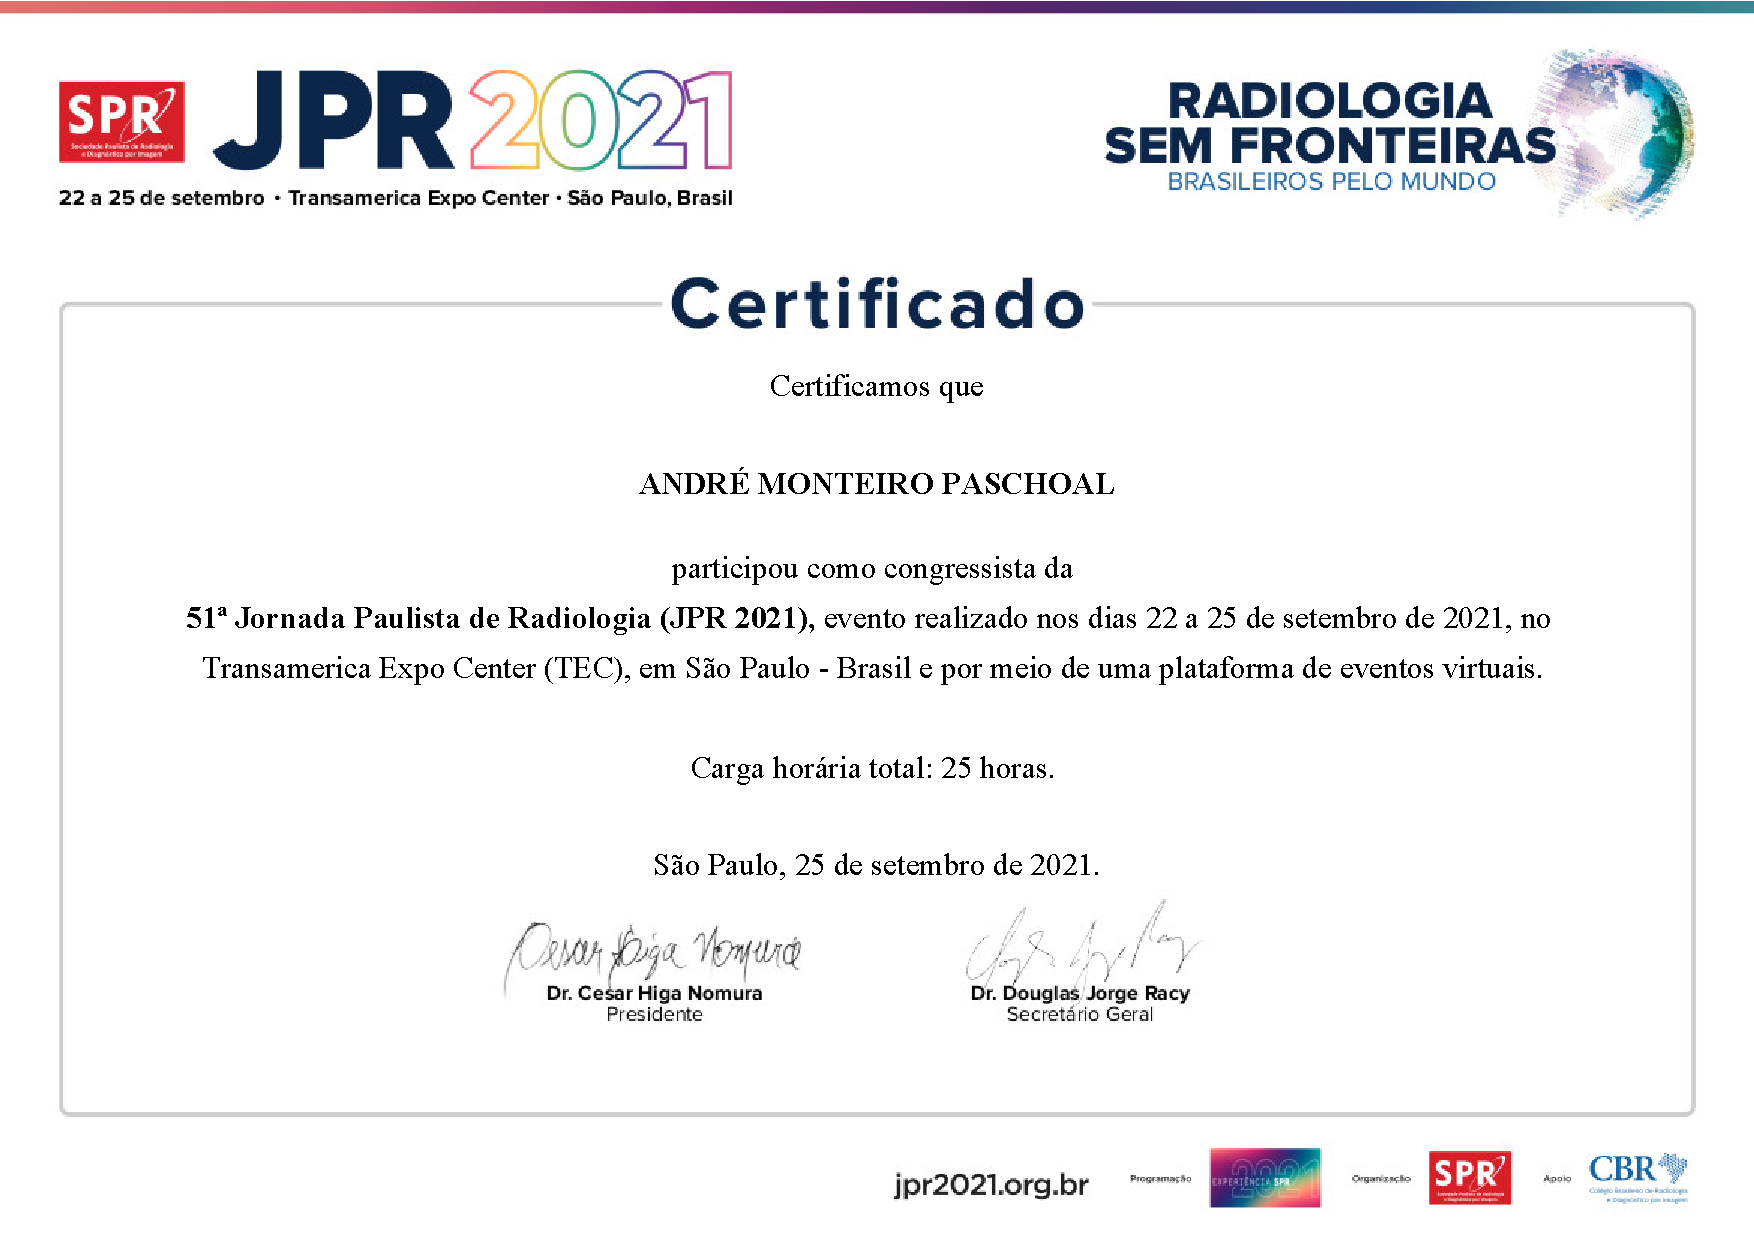
\includepdf[pages=-, scale=1,pagecommand=\thispagestyle{empty}]{\detokenize{Diplomas/JPR2021_1}}
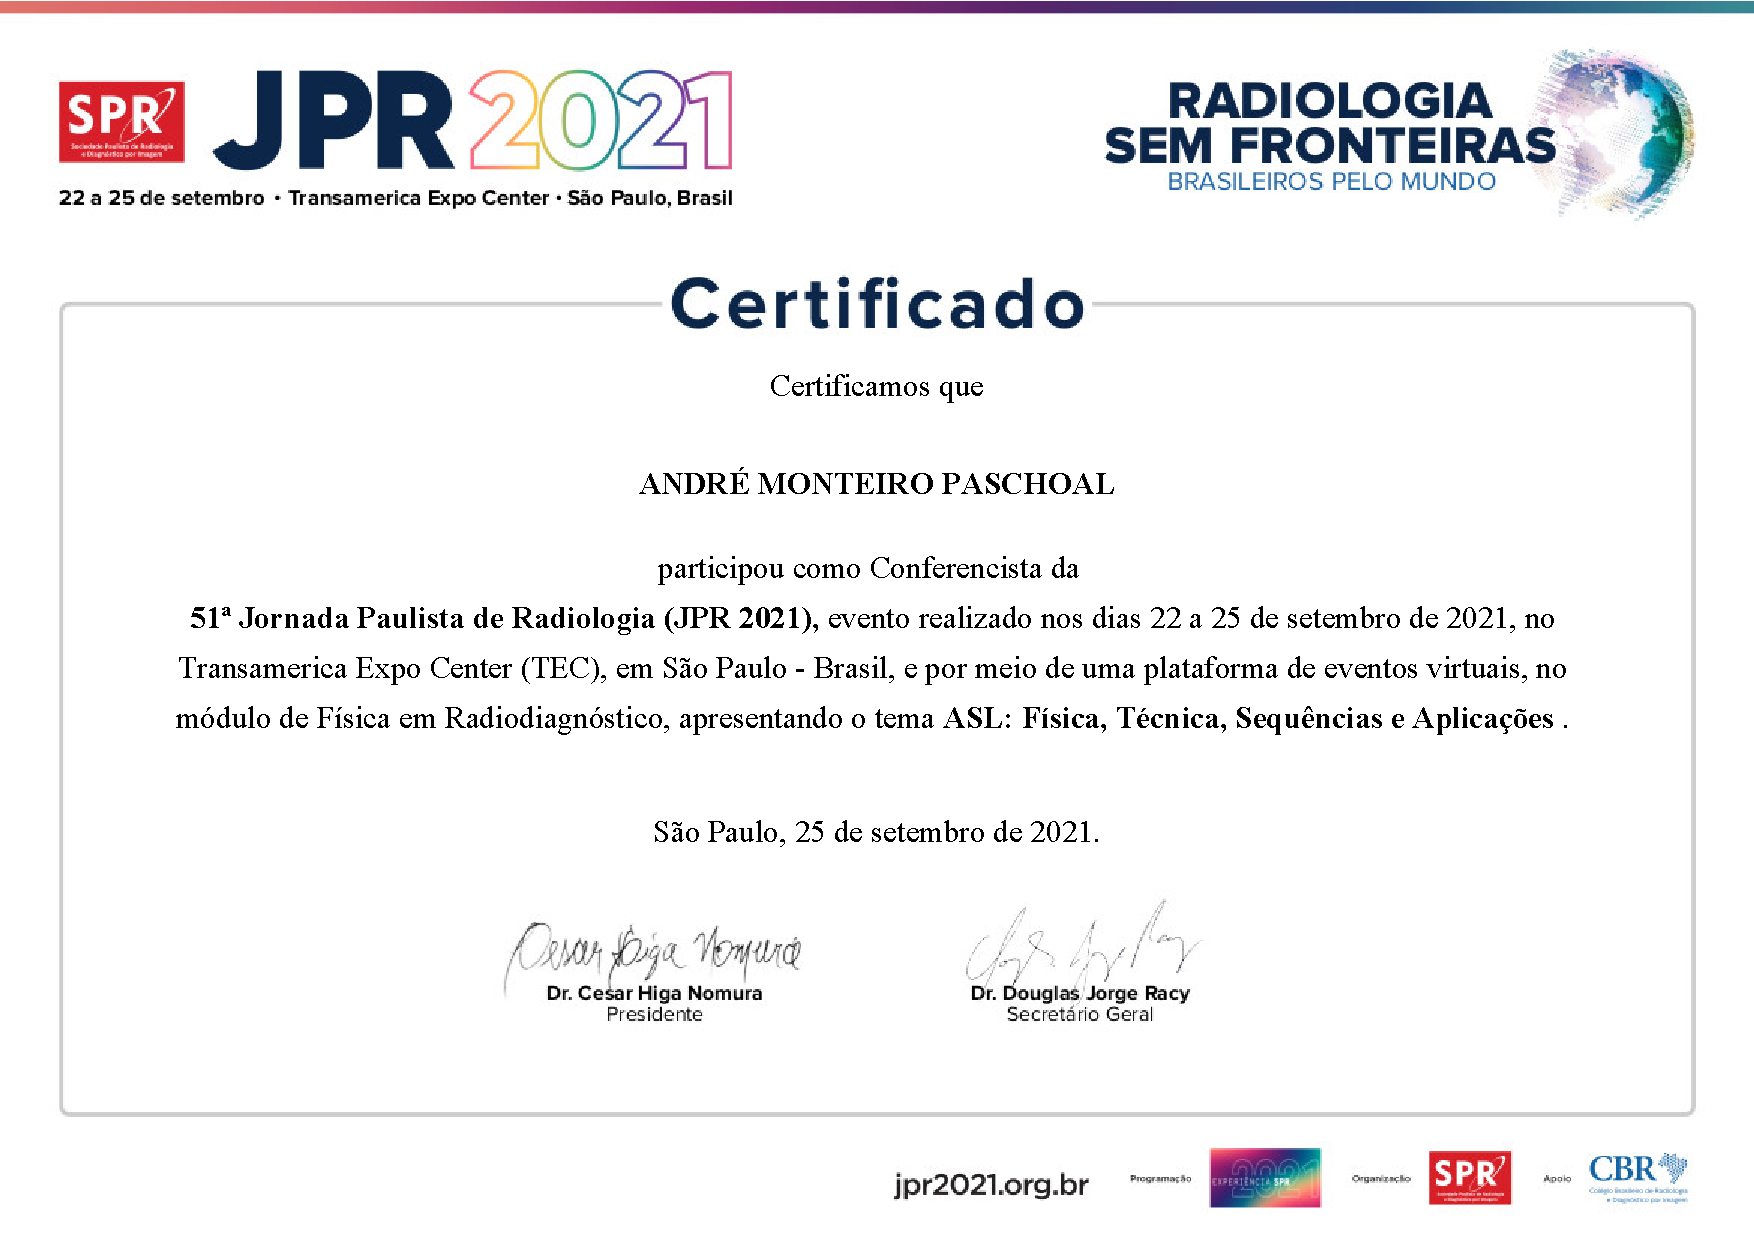
\includepdf[pages=-, scale=1,pagecommand=\thispagestyle{empty}]{\detokenize{Diplomas/JPR2021_2}}

\newpage
\subsection{Participa\c{c}\~{a}o em Eventos Cient\'{\i}ficos (com apresenta\c{c}\~{a}o de trabalho ou oferecimento de cursos, palestras ou debates}
\label{certificados:PWISMRM2022}
Esta subseção apresenta o comprovante da participação no 
ISMRM Perfusion Workshop: from head to toe com seus respectivos propósitos. \\
Obs: Ese congresso não emite certificado de apresentação de trabalhos, apenas de participação no evento.
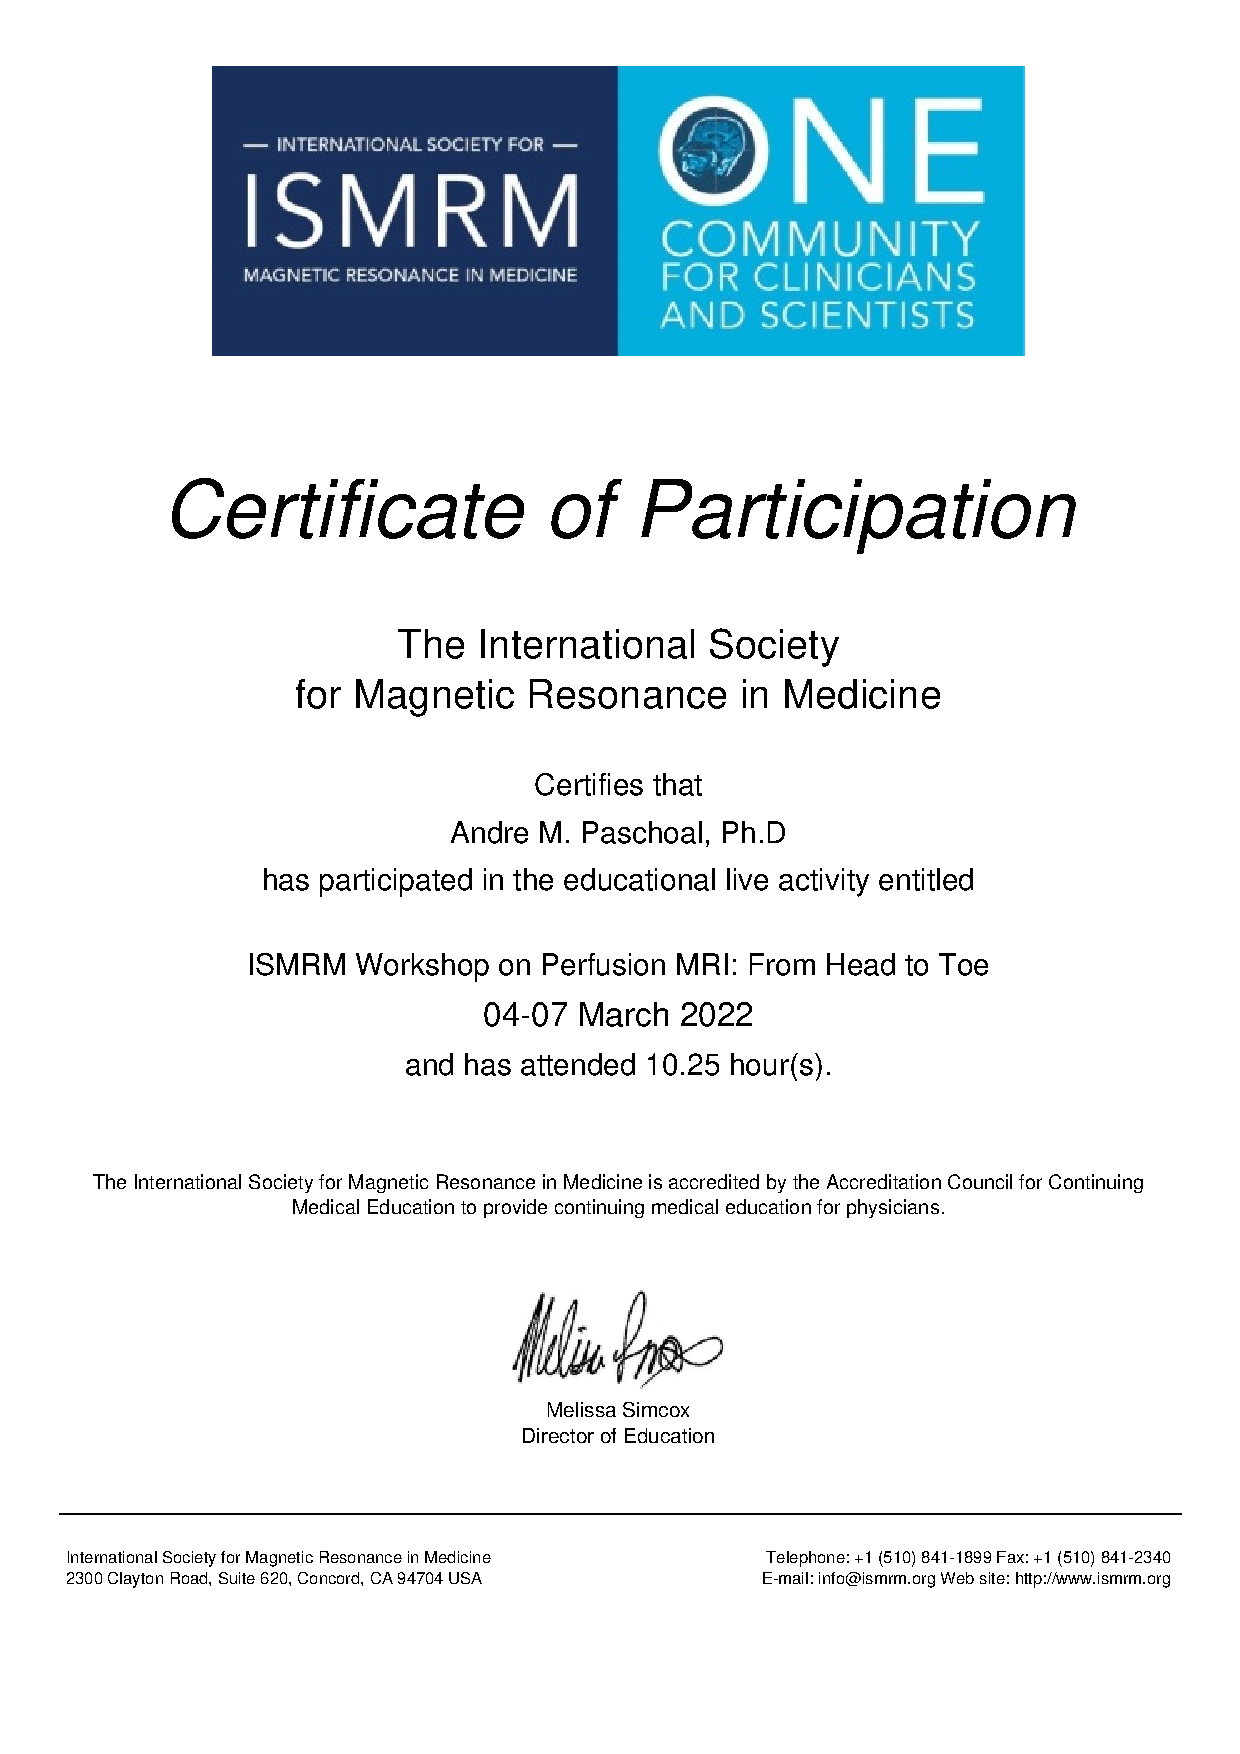
\includepdf[pages=-, scale=1,pagecommand=\thispagestyle{empty}]{\detokenize{Diplomas/PerfusionWorkshop2022_certificate}}
\includepdf[pages=-, scale=1,pagecommand=\thispagestyle{empty}]{\detokenize{Diplomas/AcceptancePWISMRM2022}}

%---

\newpage
\subsection{Obtenção  de  bolsa  de  estudo  em  instituições de  renome  científico  ou  cultural}
\label{bolsas:mestradoCAPES}
Esta subseção apresenta o comprovante de concessão da bolsa de mestrado CAPES/PROEX.
\includepdf[pages=-, scale=1,pagecommand=\thispagestyle{empty}]{\detokenize{Diplomas/mestradoCAPES}}

\newpage
\subsection{Obtenção  de  bolsa  de  estudo  em  instituições de  renome  científico  ou  cultural}
\label{bolsas:CNPQdoc}
Esta subseção apresenta o comprovante de concessão da bolsa de doutorado CNPq, processo número: 140110/2016-0.
\includepdf[pages=-, scale=1,pagecommand=\thispagestyle{empty}]{\detokenize{Diplomas/CNPq_doutorado}}

\newpage
\subsection{Obtenção  de  bolsa  de  estudo  em  instituições de  renome  científico  ou  cultural}
\label{bolsas:PDSE}
Esta subseção apresenta o comprovante de concessão da bolsa de doutorado sanduíche PDSE-CAPES, processo número: 88881.188976/2018-01.
\includepdf[pages=-, scale=1,pagecommand=\thispagestyle{empty}]{\detokenize{Diplomas/Carta de Concessão PDSE}}

\newpage
\subsection{Obtenção  de  bolsa  de  estudo  em  instituições de  renome  científico  ou  cultural}
\label{bolsas:PDJ}
Esta subseção apresenta o comprovante de concessão da bolsa de pós-doutorado junior PDJ-CNPq, processo número:  151245/2019-3.
\includepdf[pages=-, scale=1,pagecommand=\thispagestyle{empty}]{\detokenize{Diplomas/termoPDJ}}

\newpage
\subsection{Obtenção  de  bolsa  de  estudo  em  instituições de  renome  científico  ou  cultural}
\label{bolsas:TTV}
Esta subseção apresenta o comprovante de concessão da bolsa FAPESP de treinamento técnico nível V, processo número:  2020/13586-7.
\includepdf[pages=-, scale=1,pagecommand=\thispagestyle{empty}]{\detokenize{Diplomas/FAPESP_TTV}}

%---

\newpage
\subsection{Autoria de artigos completos publicados em anais de congresso, em jornais e revistas de circulação nacional e internacional na sua área}
\label{certificados:OHBM2015}
Esta subseção apresenta o comprovante da autoria do resumo publicado em anais do congresso Organization for Human Brain Mapping, 2015.
\includepdf[pages=-, scale=1,pagecommand=\thispagestyle{empty}]{\detokenize{Diplomas/AcceptanceOHBM2015}}

\newpage
\subsection{Autoria de artigos completos publicados em anais de congresso, em jornais e revistas de circulação nacional e internacional na sua área}
\label{certificados:CBFM2019}
Esta subseção apresenta o comprovante da autoria do resumo publicado em anais do congresso Brasileiro de Física Médica, 2019.
\includepdf[pages=-, scale=1,pagecommand=\thispagestyle{empty}]{\detokenize{Diplomas/AceiteCBFM2019}}

\newpage
\subsection{Autoria de artigos completos publicados em anais de congresso, em jornais e revistas de circulação nacional e internacional na sua área}
\label{certificados:ESMRMB2019}
Esta subseção apresenta o comprovante da autoria do resumo publicado em anais do congresso internacional ESMRMB 2019.
\includepdf[pages=-, scale=1,pagecommand=\thispagestyle{empty}]{\detokenize{Diplomas/AcceptanceESMRMB2019}}

%---

\newpage
\subsection{Autoria de artigos completos publicados em jornais e revistas de circulação nacional e internacional na sua área}
\label{artigos:RBFM2013}
Esta subseção apresenta o comprovante da autoria do resumo publicado em anais do congresso Brasileiro de Física Médica, 2019.
\includepdf[pages=-, scale=1,pagecommand=\thispagestyle{empty}]{\detokenize{docs/PaivaRBFM2013}}

\newpage
\subsection{Autoria de artigos completos publicados em jornais e revistas de circulação nacional e internacional na sua área}
\label{artigos:MRI2018}
Esta subseção apresenta o comprovante da autoria do artigo publicado na revista nacional \textit{Revista Brasileira de Física Médica} no ano de 2013.
\includepdf[pages=-, scale=1,pagecommand=\thispagestyle{empty}]{\detokenize{docs/silvamri2018}}

\newpage
\subsection{Autoria de artigos completos publicados em jornais e revistas de circulação nacional e internacional na sua área}
\label{artigos:NICLIN2018}
Esta subseção apresenta o comprovante da autoria do artigo publicado na revista internacional \textit{Neuroimage: clinical} no ano de 2018.
\includepdf[pages=-, scale=1,pagecommand=\thispagestyle{empty}]{\detokenize{docs/Paschoal_NeuroImageClin2018}}

\newpage
\subsection{Autoria de artigos completos publicados em jornais e revistas de circulação nacional e internacional na sua área}
\label{artigos:CONCEPTS2019}
Esta subseção apresenta o comprovante da autoria do artigo publicado na revista internacional \textit{Concepts in Magnetic Resonance Part A} no ano de 2019.
\includepdf[pages=-, scale=1,pagecommand=\thispagestyle{empty}]{\detokenize{docs/Paschoal_ConceptsPartA2019}}

\newpage
\subsection{Autoria de artigos completos publicados em jornais e revistas de circulação nacional e internacional na sua área}
\label{artigos:MAGMA2020}
Esta subseção apresenta o comprovante da autoria do artigo publicado na revista internacional \textit{Magnetic Resonance Materials in Physics, Biology and Medicine} no ano de 2020.
\includepdf[pages=-, scale=1,pagecommand=\thispagestyle{empty}]{\detokenize{docs/Paschoal2020_Article_ContrastOptimizationInArterial}}

\newpage
\subsection{Autoria de artigos completos publicados em jornais e revistas de circulação nacional e internacional na sua área}
\label{artigos:MRM2021}
Esta subseção apresenta o comprovante da autoria do artigo publicado na revista internacional \textit{Magnetic Resonance in Medicine} no ano de 2021.
\includepdf[pages=-, scale=1,pagecommand=\thispagestyle{empty}]{\detokenize{docs/mrm.28807}}

\newpage
\subsection{Autoria de artigos completos publicados em jornais e revistas de circulação nacional e internacional na sua área}
\label{artigos:JNE2021}
Esta subseção apresenta o comprovante da autoria do artigo publicado na revista internacional \textit{Journal of Neural Engineering} no ano de 2021.
\includepdf[pages=-, scale=1,pagecommand=\thispagestyle{empty}]{\detokenize{docs/jne_18_4_046089}}

\newpage
\subsection{Autoria de artigos completos publicados em jornais e revistas de circulação nacional e internacional na sua área}
\label{artigos:JMRI2021}
Esta subseção apresenta o comprovante da autoria do artigo publicado na revista internacional \textit{Journal of Magnetic Resonance Imaging} no ano de 2021.
\includepdf[pages=-, scale=1,pagecommand=\thispagestyle{empty}]{\detokenize{docs/jmri.27899}}

\newpage
\subsection{Autoria de artigos completos publicados em jornais e revistas de circulação nacional e internacional na sua área}
\label{artigos:MAGMA2021}
Esta subseção apresenta o comprovante da autoria do artigo publicado na revista internacional \textit{Magnetic Resonance Materials in Physics, Biology and Medicine} no ano de 2021.
\includepdf[pages=-, scale=1,pagecommand=\thispagestyle{empty}]{\detokenize{docs/Paschoal2022_Article_FeasibilityOfIntravoxelIncoher}}

\newpage
\subsection{Autoria de artigos completos publicados em jornais e revistas de circulação nacional e internacional na sua área}
\label{artigos:NMRBiomed2022_2}
Esta subseção apresenta o comprovante da autoria do artigo publicado na revista internacional \textit{NMR in Biomedicine} no ano de 2022.
\includepdf[pages=-, scale=1,pagecommand=\thispagestyle{empty}]{\detokenize{docs/NBM-22-0068}}

\newpage
\subsection{Autoria de resumo aceito para apresentação em congresso, em jornais e revistas de circulação nacional e internacional na sua área}
\label{certificados:ISMRM2022_1}
Esta subseção apresenta o comprovante de aceite de resumo a ser apresentado no congresso internacional ISMRM 2022.
\includepdf[pages=-, scale=1,pagecommand=\thispagestyle{empty}]{\detokenize{Diplomas/Acceptance_ISMRM2022_1}}
\includepdf[pages=-, scale=1,pagecommand=\thispagestyle{empty}]{\detokenize{docs/ISMRM2022_MS}}

\newpage
\subsection{Autoria de resumo aceito para apresentação em congresso, em jornais e revistas de circulação nacional e internacional na sua área}
\label{certificados:ISMRM2022_2}
Esta subseção apresenta o comprovante de aceite de resumo a ser apresentado no congresso internacional ISMRM 2022.
\includepdf[pages=-, scale=1,pagecommand=\thispagestyle{empty}]{\detokenize{Diplomas/Acceptance_ISMRM2022_2}}
\includepdf[pages=-, scale=1,pagecommand=\thispagestyle{empty}]{\detokenize{docs/ISMRM2022_OSIPI}}

\newpage
\subsection{Autoria de resumo aceito para apresentação em congresso, em jornais e revistas de circulação nacional e internacional na sua área}
\label{certificados:BRAINN2022}
Esta subseção apresenta o comprovante de aceite de resumo a ser apresentado no congresso internacional 8th BRAINN Congress 2022.
\includepdf[pages=-, scale=1,pagecommand=\thispagestyle{empty}]{\detokenize{Diplomas/Acceptance_BRAINN2022}}
\includepdf[pages=-, scale=1,pagecommand=\thispagestyle{empty}]{\detokenize{docs/BRAIN2022}}

\newpage
\subsection{Autoria de resumo aceito para apresentação em congresso, em jornais e revistas de circulação nacional e internacional na sua área}
\label{certificados:JPR2022}
Esta subseção apresenta o comprovante de participação em palestra a ser apresentada no congresso Jornada Paulista de Radiologia 2022.
\includepdf[pages=-, scale=1,pagecommand=\thispagestyle{empty}]{\detokenize{Diplomas/JPR2022}}

%---

\newpage
\subsection{Atividades de docência}
\label{aulas:EEP}
Esta subseção apresenta o certificado de atividades como docente no curso de Especialização em Ressonância Magnética para Biomédicos e Tecnólogos pela Escola de 
Educação Permanente do Hospital das Clínicas da Faculdade de Medicina da Universidade de São Paulo nos anos de 2021 e 2022, ministrando as disciplinas de física básica e física avançada.
\includepdf[pages=-, scale=1,pagecommand=\thispagestyle{empty}]{\detokenize{Diplomas/aulasEEP}}

\newpage
\subsection{Monitorias para disciplinas de graduação}
\label{monitorias:IFSC}
Esta subseção apresenta o comprovante de Monitoria para alunos de graduação.
\includepdf[pages=-, scale=1,pagecommand=\thispagestyle{empty}]{\detokenize{Diplomas/MonitoriaIFSC}}

\newpage
\subsection{Monitorias para disciplinas de graduação}
\label{monitorias:FFCLRP}
Esta subseção apresenta o comprovante de Monitoria para alunos de graduação.
\includepdf[pages=-, scale=1,pagecommand=\thispagestyle{empty}]{\detokenize{Diplomas/monitoriaPIM_2017_1FFCLRP}}

\newpage
\subsection{Monitorias para disciplinas de graduação}
\label{monitorias:PAE1}
Esta subseção apresenta o comprovante de Monitoria para alunos de graduação.
\includepdf[pages=-, scale=1,pagecommand=\thispagestyle{empty}]{\detokenize{Diplomas/monitoriaPAE_2017_2FFCLRP}}

\newpage
\subsection{Monitorias para disciplinas de graduação}
\label{monitorias:PAE2}
Esta subseção apresenta o comprovante de Monitoria para alunos de graduação.
\includepdf[pages=-, scale=1,pagecommand=\thispagestyle{empty}]{\detokenize{Diplomas/monitoriaPAE_2019_2FFCLRP}}

%---

\newpage
\subsection{Membro de Comissão Avaliadora}
\label{avaliador:SIICUSP2019}
Esta subseção apresenta o comprovante de participação em comissão avaliadora de eventos.
\includepdf[pages=-, scale=1,pagecommand=\thispagestyle{empty}]{\detokenize{Diplomas/certificado_siicusp}}

\newpage
\subsection{Membro de Comissão Avaliadora}
\label{avaliador:SFM2019}
Esta subseção apresenta o comprovante de participação em comissão avaliadora de eventos.
\includepdf[pages=-, scale=1,pagecommand=\thispagestyle{empty}]{\detokenize{Diplomas/certificadoAvaliador_SFM2019}}

\newpage
\subsection{Membro de Comissão Avaliadora}
\label{avaliador:SIICUSP2020}
Esta subseção apresenta o comprovante de participação em comissão avaliadora de eventos.
\includepdf[pages=-, scale=1,pagecommand=\thispagestyle{empty}]{\detokenize{Diplomas/SIICUSP2020}}

%---

%%%%%%%%%%%%%%%%%%%%%%%%%%%%%%%%%%%%%%%%%%%%%%%%%%%%%%%%%%%%%%%%%%%%%%%%%%%%%%%
% Subgrupo 3.2 - Coordenação de Eventos e Conferencista
%%%%%%%%%%%%%%%%%%%%%%%%%%%%%%%%%%%%%%%%%%%%%%%%%%%%%%%%%%%%%%%%%%%%%%%%%%%%%%%

%\newpage
%\subsection{Comiss\~{a}o Organizadora de Eventos Internacional, Nacional, Regional ou Local}
%\label{reviewer:2015-sbcars}
%Esta subseção apresenta o comprovante de Comiss\~{a}o Organizadora do 9th Brazilian Symposium on Software Components, Architectures and Reuse (SBCARS 2015).
%\includepdf[pages=-, scale=1,pagecommand=\thispagestyle{empty}]{\detokenize{GRUPO 3/Sub-Grupo 32/Comprovante Fake}}

%%%%%%%%%%%%%%%%%%%%%%%%%%%%%%%%%%%%%%%%%%%%%%%%%%%%%%%%%%%%%%%%%%%%%%%%%%%%%%%
% Grupo 4: Atividades de Forma\c{c}\~{a}o e Capacita\c{c}\~{a}o Acad\^{e}mica
%%%%%%%%%%%%%%%%%%%%%%%%%%%%%%%%%%%%%%%%%%%%%%%%%%%%%%%%%%%%%%%%%%%%%%%%%%%%%%%

\newpage
\subsection{Comiss\~{a}o Organizadora de Eventos Internacional, Nacional, Regional ou Local}
\label{organizacao:inbrain}
Esta subseção apresenta o comprovante de Participação de Comissão Organizadora de Eventos Nacionais e Internacionais.
\includepdf[pages=-, scale=1,pagecommand=\thispagestyle{empty}]{\detokenize{Diplomas/InBrainWorkshop_organizacao}}

\newpage
\subsection{Comiss\~{a}o Organizadora de Eventos Internacional, Nacional, Regional ou Local}
\label{organizacao:eifamb}
Esta subseção apresenta o comprovante de Participação de Comissão Organizadora de Eventos Nacionais e Internacionais.
\includepdf[pages=-, scale=1,pagecommand=\thispagestyle{empty}]{\detokenize{Diplomas/EIFAMB2018_CO_AndréMonteiroPaschoal}}

%------------------------------------------------------------------------------
%%%%%%%%%%%%%%%%%%%%%%%%%%%%%%%%%%%%%%%%%%%%%%%%%%%%%%%%%%%%%%%%%%%%%%%%%%%%%%%
% \newpage
% \subsection{Portaria de Progressão}
% \label{app:2014-portaria-progressao}
% \includepdf[pages=-, scale=1,pagecommand=\thispagestyle{empty}]{\detokenize{GRUPO 1/20141205_Portaria-de-Progressao-Funcional_5929-2014.pdf}}


\end{document}

%%% EOF
